% -----------------------------------------------------------------------
% Template Skripsi untuk MIPA
% 
% @author Yusuf Syaifudin
% @created 29/02/2016
% 
% -----------------------------------------------------------------------

\documentclass[ugmskripsi]{ugmskripsi}

% ------------------------------------------------------------------------------
% Berisi tambahan package dan konfigurasi untuk masing-masing package.
% Ada baiknya, setiap konfigurasi diletakkan tepat dibawah 
% setelah package dilakukan import (usepackage) agar tidak membingungkan.
% Serta disarankan untuk menambah kegunaan package tersebut agar tidak lupa.
% ------------------------------------------------------------------------------

% For \colorbox[RGB]{218,232,252}{warna biru}
% For \colorbox[RGB]{213,232,212}{warna hijau}
\usepackage[dvipsnames]{xcolor}

% font tambahan
\usepackage{textcomp}

% untuk math
\usepackage{amssymb}


% digunakan untuk membuat flowchart
\usepackage{tikz}
\usetikzlibrary{shapes, shapes.misc, arrows, fit, positioning}
\tikzstyle{block} = [rectangle, draw, fill=gray!20, text width=4cm, text centered, rounded corners, minimum height=3em]
\tikzstyle{io} = [trapezium, draw, fill=gray!20, text width=1cm, text centered, rounded corners, minimum height=3em]
\tikzstyle{decision} = [diamond, draw, fill=gray!20, text width=3cm, text centered, minimum height=3em]

\usepackage{float}
\usepackage{booktabs}
\usepackage{pbox}
\usepackage{multirow}
\usepackage[normalem]{ulem}
\useunder{\uline}{\ul}{}

% Untuk hyperlink dan otomatis membuat bookmark
\usepackage{hyperref}

% break tanda /, - dan spasi ke baris baru jika sudah tidak muat
\def\UrlBreaks{\do\/\do-\do\ }

% font url dibuat miring dan dg jenis font ttfamily
\renewcommand{\UrlFont}{\small\ttfamily\itshape}

\usepackage{csquotes}
\usepackage{framed}
\usepackage{enumitem}

% untuk input kode baik dari file atau bukan
\usepackage{listings}

% ----------------------------------------------------------------------------
% Contoh dari file
% ----------------------------------------------------------------------------
% \begin{figure}[H]
%   \lstinputlisting[language=python, firstline=38, lastline=59]{code/linkwalker.py}
%   \caption{Mendapatkan daftar tautan berita pada kompas.com}
%   \label{grab daftar berita kompas}
% \end{figure}
% ----------------------------------------------------------------------------
%
% ----------------------------------------------------------------------------
% Contoh
% ----------------------------------------------------------------------------
% \begin{figure}
% 	\begin{lstlisting}[language=sql]
% 		update train_data_statement set data = replace(data, '“', '"');
% 		update train_data_statement set data = replace(data, '”', '"');

% 		update test_data_statement set data = replace(data, '“', '"');
% 		update test_data_statement set data = replace(data, '”', '"');
% 	\end{lstlisting}
% 	\caption{\textit{Query} SQL untuk melakukan perubahan karakter pada data}
% 	\label{kueri SQL untuk melakukan perubahan karakter pada data}
% \end{figure}
% ------------------------------------------------------------------------------

\usepackage{color}
\usepackage{amsmath}
\usepackage{courier}
\usepackage[scaled=.75]{beramono}

%-----------------------------------------------------------------
% Setting syntax hightlighting
%-----------------------------------------------------------------
\lstset{frame=tb,
  language=Python,
  aboveskip=2mm,
  belowskip=1mm,
  showstringspaces=false,
  columns=flexible,
  basicstyle  = \fontfamily{pcr}\fontsize{8pt}{8pt}\selectfont,
  numbersep=8pt,
  numbers=left,
  numberstyle=\tiny\color{gray},
  keywordstyle=\color{blue},
  commentstyle=\color{dkgreen},
  stringstyle=\color{mauve},
  breaklines=true,
  breakatwhitespace=true,
  tabsize=4
}

% Untuk menghilangkan titik-titik pada daftar isi

\usepackage[titles]{tocloft}
\renewcommand{\cftdot}{}

% Untuk membuat multi kolom
\usepackage{etoolbox,refcount}
\usepackage{multicol}

% Konfigurasi multi kolom
% bikin multi kolom
\newcounter{countitems}
\newcounter{nextitemizecount}
\newcommand{\setupcountitems}{%
  \stepcounter{nextitemizecount}%
  \setcounter{countitems}{0}%
  \preto\item{\stepcounter{countitems}}%
}
\makeatletter
\newcommand{\computecountitems}{%
  \edef\@currentlabel{\number\c@countitems}%
  \label{countitems@\number\numexpr\value{nextitemizecount}-1\relax}%
}
\newcommand{\nextitemizecount}{%
  \getrefnumber{countitems@\number\c@nextitemizecount}%
}
\newcommand{\previtemizecount}{%
  \getrefnumber{countitems@\number\numexpr\value{nextitemizecount}-1\relax}%
}
\makeatother
\newenvironment{AutoMultiColItemize}{%
\ifnumcomp{\nextitemizecount}{>}{2}{\begin{multicols}{2}}{}%
\setupcountitems\begin{itemize}}%
{\end{itemize}%
\unskip\computecountitems\ifnumcomp{\previtemizecount}{>}{2}{\end{multicols}}{}}
%end bikin multi kolom

% ------------------------------------------------------------------------------
% Contoh sintaks:
% ------------------------------------------------------------------------------
% \begin{itemize}
%   \item \textit{Reporting verb} yang hadir sebelum entitas pada kutipan langsung:
%   \begin{AutoMultiColItemize}
% 	  \item tutur
% 	  \item kata
% 	  \item ujar
%   \end{AutoMultiColItemize}

%   \item \textit{Reporting verb} yang hadir setelah entitas pada kutipan langsung:
%   \begin{AutoMultiColItemize}
% 	  \item mengatakan
% 	  \item menjawab
%   \end{AutoMultiColItemize}
% \end{itemize}
% ------------------------------------------------------------------------------


% Setting list agar spasi antar list tidak terlalu banyak
\setlist{
listparindent=\parindent,
parsep=0pt
}

% Agar tetap Justify tapi kata tidak dipisah sesuka hati (not hypenation but justified)
\tolerance=1
\emergencystretch=\maxdimen
\hyphenpenalty=10000
\hbadness=10000
\hyphenchar\font=-1
\sloppy

% Agar support longtable
% https://tex.stackexchange.com/questions/639452/create-long-table-in-latex
% need: varwidth, ninecolors
%%%% begin of required preamble
\usepackage{tabularray}
\UseTblrLibrary{varwidth}
\DefTblrTemplate{contfoot-text}{default}{Bersambung di halaman selanjutnya}
\DefTblrTemplate{conthead-text}{default}{(Lanjutan)}

% https://stackoverflow.com/a/16804893
% \usepackage{tablefootnote}
% \usepackage{footnote}
% \makesavenoteenv{tabular}
% \makesavenoteenv{table}

\usepackage{amsmath}   % <-- for \eqref

\usepackage{pgfgantt}


% for \includepdf
\usepackage{pdfpages}
\usepackage{longtable}

\usepackage{graphicx}    
\usepackage{subcaption}  

\usepackage{algorithm} 
\usepackage{algpseudocode}
\usepackage{amsmath, amsthm}
\usepackage{adjustbox}


% Konfigurasi variable seperti judul dan lain sebagainya
\titleind{Pembuatan Perangkat Lunak  \textit{Traffic Aware Routing Engine} untuk Openstreetmap dengan menggunakan \textit{Time-dependent Customizable Route Planning}, \textit{Graph Neural Network}, dan \textit{Bayesian Filtering}}

\titleeng{Development of Traffic Aware Routing Engine Software for Openstreetmap using Time-dependent Customizable Route Planning, Graph Neural Network, and Bayesian Filtering}

\fullname{Lintang Birda Saputra}

\idnum{22/505034/PA/21737}

\examdate{27 September 2025}

\degree{Sarjana Komputer}

\yearsubmit{2025}

\program{Ilmu Komputer}

\gelar{Sarjana Komputer}

\headprogram{Azhari SN, Dr., MT}

\dept{Ilmu Komputer dan Elektronika}

\firstsupervisor{Faizal Makhrus, S.Kom., M.Sc., Ph.D.}

\firstexaminer{Mhd. Reza M.I Pulungan, M.Sc., Dr.-Ing}

\secondexaminer{Sigit Priyanta, S.Si., M.Kom}



\begin{document}

%-----------------------------------------------------------------
% Disini awal masukan untuk muka skripsi
%-----------------------------------------------------------------

% Cover
\cover

% Halaman judul
\titlepageind 

% Halaman Persetujuan
\approvalpage

% Halaman Pernyataan
\declarepage

% Halaman Persembahan
\acknowledment
\begin{flushright}
\Large\emph\cal{Karya ini ku persembahkan kepada \\
Ibu, Bapak, dan Kakak}
\end{flushright}

%-----------------------------------------------------------------
% Disini akhir masukan untuk muka skripsi
%-----------------------------------------------------------------

% Motto
\input{BAB_SKRIPSI/BAB0/2_MOTTO}

% Prakata
\input{BAB_SKRIPSI/BAB0/3_PRAKATA}

%-----------------------------------------------------------------
% Daftar Isi
%-----------------------------------------------------------------
\newpage
\phantomsection
\addcontentsline{toc}{chapter}{\contentsname}
\tableofcontents
%-----------------------------------------------------------------
% Akhir Daftar Isi
%-----------------------------------------------------------------

%-----------------------------------------------------------------
% Daftar Tabel
%-----------------------------------------------------------------
\newpage
\phantomsection
\addcontentsline{toc}{chapter}{\listtablename}
\listoftables
%-----------------------------------------------------------------
% Akhir Daftar Tabel
%-----------------------------------------------------------------

%-----------------------------------------------------------------
% Daftar Gambar
%-----------------------------------------------------------------
\newpage
\phantomsection
\addcontentsline{toc}{chapter}{\listfigurename}
\listoffigures
%-----------------------------------------------------------------
% Akhir Daftar Gambar
%-----------------------------------------------------------------


%-----------------------------------------------------------------
%Disini awal masukan Intisari
%-----------------------------------------------------------------
\begin{abstractind}
	\input{BAB_SKRIPSI/BAB0/4_ABSTRAK_ID}
\end{abstractind}
%-----------------------------------------------------------------
%Disini akhir masukan Intisari
%-----------------------------------------------------------------

%-----------------------------------------------------------------
%Disini awal masukan untuk Abstract
%-----------------------------------------------------------------
\begin{abstracteng}
  \input{BAB_SKRIPSI/BAB0/5_ABSTRAK_EN}
\end{abstracteng}
%-----------------------------------------------------------------
%Disini akhir masukan Abstract
%-----------------------------------------------------------------


%-----------------------------------------------------------------
% Awal BAB 1
%-----------------------------------------------------------------
\chapter{PENDAHULUAN}
\label{PENDAHULUAN}

	\section{Latar Belakang}
	\label{pendahuluan latar belakang}
	Algoritma Komputer saat ini digunakan dalam berbagai bidang untuk meningkatkan efektifitas pekerjaan dan taraf hidup manusia. Salah satu bidang yang saat ini sedang berkembang dengan pesat adalah \textit{route planning} dengan menggunakan modifikasi dari algoritma dijkstra untuk mencari rute optimal dengan cepat. 

Menghitung rute optimal di dalam jaringan transportasi memiliki banyak aplikasi di dunia nyata, kita sering menggunakan fungsi ini untuk merencakanan perjalanan dengan kendaraan, terdapat juga aplikasi lain seerti perencanaan logistik dan transportasi publik.

Meskipun algoritma klasik dijkstra (\cite{Dijkstra59}) berjalan dalam waktu yang hampir linier, penerapannya pada graph berukuran benua memerlukan beberapa detik sehingga tidak bisa digunakan untuk aplikasi \textit{real-time}. Hal ini memotivasi banyak penelitian (\cite{Delling2009} dan \cite{Bast2015}) tentang metode akselerasi yang membagi pekerjaan perencanaan rute menjadi dua tahap: langkah \textit{preprocessing}, yang mungkin memakan waktu beberapa menit atau bahkan berjam-jam untuk menhasilkan kumpulan data tambahan yang dapat mempercepat proses kueri, tahap  kedua berupa fase kueri yang dapat dijawab dalam hitungan milidetik. Sebagian besar penelitian sebelumnya telah diuji pada jaringan jalan di Eropa dan Amerika Serikat menggunakan waktu tempuh sebagai kriteria optimasi utama.

Terdapat juga beberapa metode yang dapat mempertimbangkan histori kondisi lalu lintas dan keadaan lalu lintas terkini (\cite{DellingTD2009}, \cite{Baum2016}, dan \cite{Veit2013}) yang mana mengganti bobot dari \textit{edge} dengan menggunakan \textit{travel time function} $f : \mathbb{R} \to \mathbb{R}_{\geq 0}$, lalu menggunakan \textit{time-dependent dijkstra} dan \textit{profile search} untuk melakukan kueri dan \textit{preprocessing}. Performa dari berbagai metode \textit{time-dependent route planning} dapat menyamai performa dari \textit{time-independent route planning} di berbagai data jaringan jalan. Salah satu penelitian di bidang ini adalah penelitian oleh \cite{Delling2015} yang menggunakan metode \textit{customizable route planning}, dimana metode ini dibagi menjadi 3 tahap, yaitu praproses, kustomisasi, dan kueri. Praproses mempartisi graf jaringan jalan menjadi beberapa partisi, kustomisasi menghitung rute terpendek dari semua pasangan simpul yang berada pada batas partisi, dan kueri menjalankan kueri dalam hitungan beberapa milidetik. Kustomisasi pada metode \textit{Customizable Route Planning} dapat dilakukan hanya dalam hitungan beberapa detik, yang memungkinkan perbaruan data graf menyesuaikan kondisi lalu lintas. Penelitian oleh \cite{Baum2016} melakukan ekstensi dari metode \textit{Customizable Route Planning} dimana kueri dapat mempertimbangkan kondisi trafik pada masa mendatang.

Dalam konteks aplikasi \textit{routing engine}, \textit{map matching} memiliki peranan yang sangat penting karena kualitas hasil perencanaan rute sangat bergantung pada akurasi posisi pengguna pada jaringan jalan. \textit{Map matching} adalah proses mencocokkan titik-titik lokasi hasil pelacakan GPS dengan ruas jalan yang sebenarnya pada graf jaringan transportasi (\cite{Newson2009}). Data GPS yang mentah sering kali mengandung error, seperti deviasi posisi akibat gangguan sinyal satelit, sehingga posisi pengguna tidak selalu tepat berada di atas ruas jalan. Tanpa proses \textit{map matching}, sistem rute dapat menghasilkan jalur yang keliru, misalnya menempatkan kendaraan di jalan paralel yang berbeda atau memberikan instruksi navigasi dan pengalihan rute yang tidak relevan.


Banyak penelitian mengenai \textit{map matching} yang sudah dilakukan sebelumnya. Salah satu metode \textit{map matching} yang paling sering digunakan adalah Hidden Markov Model yang diperkenalkan pada penelitian oleh \cite{Newson2009}, dimana setiap trajektori titik gps diperlakukan sebagai observasi, sedangkan posisi sbeenarnya pada ruas jalan dianggap sebagai \textit{hidden states}. Dengan memanfaatkan probabilitas emisi (kedekatan titik GPS dengan kandidat jalan) dan probabilitas transisi (kemungkinan berpindah antar ruas jalan), algoritma viterbi dapat digunakan untuk menemukan jalur optimal yang sesuai dengan trajektori GPS.

Selain metode Hidden Markov Model yang mana hanya dapat melakukan \textit{map matching} secara \textit{offline}, terdapat juga pendekatan \textit{Candidate-Evolving Model} yang mempertahankan sekumpulan kandidat jalur dan memperbaruinya seiring dengan bertambahnya titik GPS baru. Salah satu metode representatif dari kategori ini adalah \textit{Multiple Hypothesis Technique (MHT)} yang diperkenalkan pada penelitian oleh \cite{Taguchi2019}. MHT berfokus pada pemeliharaan daftar hipotesis kandidat jalan dengan biaya komputasi yang lebih rendah. Setiap hipotesis dievaluasi menggunakan fungsi skor yang mempertimbangkan kesesuaian antara titik GPS dan kandidat jalan terdekat, kemudian daftar hipotesis diperbarui untuk memastikan kemungkinan jalur yang benar tetap terjaga. Keunggulan dari metode ini adalah kemampuannya untuk diadaptasikan dalam skenario \textit{online map matching}, termasuk melakukan prediksi jalur ke depan berdasarkan hipotesis yang ada. 

Terdapat juga beberapa perangkat lunak sumber terbuka untuk perencanaan rute pada openstreetmap. Perangkat lunak Open Source Routing Machine (OSRM)  (\cite{Luxen2011}) menggunakan pendekatan yang mirip dengan Customizable Route Planning (\cite{Delling2015}) dan juga mampu melakukan kueri dalam hitungan beberapa milidetik dan mampu melakukan kustomisasi dalam hitungan beberapa detik.



Mayoritas perangkat lunak sumber terbuka untuk \textit{route planning} pada Openstreetmap berfokus pada \textit{time-independent route planning} dan tidak mengintegrasikannya dengan model \textit{traffic speed forecasting} sehingga hasil kueri dari perangkat lunak ini tidak mempertimbangkan kondisi lalu lintas pada masa depan. Juga pada perangkat lunak ini, tidak terdapat fitur \textit{online map matching}, yaitu menentukan lokasi yang sebenarnya pada ruas jalan pada jaringan jalan dari data trajektori GPS secara \textit{real-time}.

Pada penelitian ini akan dibahas pengembangan perangkat lunak \textit{routing engine} untuk Openstreetmap yang menyediakan fitur \textit{time-dependent} \textit{route-planning} dan \textit{online map-matching}. Penelitian ini juga membahas permasalahan, limitasi, serta peningkatan dari metode-metode pada penelitian sebelumnya.




	\section{Rumusan Masalah}
	\label{pendahuluan rumusan masalah}
	Penggunaan algoritma dan teknik akselerasi dalam beberapa perangkat lunak \textit{routing engine} terbukti mampu mempercepat proses pencarian rute terpendek hingga beberapa kali lipat dibandingkan dengan algoritma Dijkstra standar. Namun, sebagian besar metode tersebut masih diterapkan pada jaringan jalan time-independent, yaitu kondisi di mana bobot setiap sisi (misalnya waktu tempuh pada segmen jalan) dianggap konstan dan tidak berubah seiring waktu. Asumsi time-independent ini menyebabkan hasil rute terpendek yang diperoleh tidak mempertimbangkan variasi kondisi lalu lintas, baik berdasarkan prediksi maupun data historis. Akibatnya, rute yang dipilih berpotensi tidak optimal, terutama ketika dalam jangka waktu dekat terjadi peningkatan kepadatan lalu lintas atau kemacetan yang signifikan. Penggunaan algoritma dan metode untuk map matching yang diimplementasikan pada beberapa perangkan lunak sumber terbuka terbukti mampu menghasilkan trajektori lintasan yang akurat pada jaringan jalan, namun kebanyakan solusi yang ada hanya bisa dilakukan secara \textit{offline}, yaitu rute harus diselesaikan dulu sebelum bisa melakukan \textit{map-matching}, padahal kebanyakan aplikasi navigasi seperti Google Maps dan Apple Maps melakukan \textit{map-matching} secara \textit{real-time}. Untuk itu perlu adanya perangkat lunak \textit{routing engine} untuk mengatasi permasalahan diatas.


	\section{Batasan Masalah}
	\label{pendahuluan batasan masalah}
	\begin{enumerate}
    \item Pembuatan software traffic aware routing engine menggunakan Time-Depdendent Customizable Route Planning, rute alternative, dan online map-matching dengan Multiple Hypothesis Technique (MHT) dengan bahasa pemrograman Go dan Typescript.
    \item Pembuatan model dari Graph Neural Network menggunakan library PyTorch.
    \item Algoritma yang dibandingkan adalah time-independent Customizable Route Planning, Contraction Hierarchies, dan Time-dependent Customizable Route Planning.
    \item Pengujian algoritma dilakukan pada beberapa query rute terpendek dan rute alternatif yang digenerate secara acak pada peta openstreetmap dengan batas wilayah area Dareah Istimewa Yogyakarta, Klaten, dan Surakarta. 
    \item Dataset histori traffic speed diperoleh dengan melakukan simulasi traffic dengan software sumo dalam kurun waktu simulasi 30 hari.
    \item Arsitektur Graph Neural Network yang digunakan adalah Dynamic Graph Convolutional Recurrent Network.
\end{enumerate}

	\section{Tujuan Penelitian}
	\label{pendahuluan tujuan penelitian}
	\begin{enumerate}
    \item Mengembangkan mesin perutean (routing engine) berbasis Time-Dependent Customizable Route Planning (TDCRP) yang mampu menghasilkan rute terpendek dan rute alternatif dengan mempertimbangkan variasi kondisi lalu lintas.
    \item Membandingkan performa algoritma Time-Independent CRP, Contraction Hierarchies (CH), dan Time-Dependent CRP dalam hal waktu prapemrosesan, waktu kueri, serta kualitas rute yang dihasilkan.
    \item Mengembangkan fitur \textit{online map-matching} yang mampu menghasilkan      prediksi trajektori pada ruas jalan jaringan jalan berdasarkan trajektori GPS.
    \item  Membangun dan menerapkan model Graph Neural Network (Dynamic Graph Convolutional Recurrent Network) untuk memodelkan dan memprediksi kondisi lalu lintas berdasarkan data historis dari hasil simulasi.
    \item Mengintegrasikan prediksi kondisi lalu lintas dari GNN ke dalam fungsi biaya pada TDCRP, sehingga mesin perutean mampu menghasilkan rute yang lebih optimal secara kontekstual.   
    \item Menyediakan prototipe perangkat lunak perutean yang dapat dijalankan secara interaktif, berbasis bahasa pemrograman Go (backend), Python (Machine Learning), dan TypeScript (frontend), untuk mendemonstrasikan hasil penelitian.
\end{enumerate}

	\section{Manfaat Penelitian}
	\label{pendahuluan manfaat penelitian}
	Penelitian pengembangan perangkat lunak \textit{traffic aware routing engine} pada \textit{openstreetmap} dilakukan untuk menghasilkan rute yang lebih optimal dan kontekstual dibandingkan dengan \textit{time-independent routing engine} yang selama ini banyak digunakan pada perangkat lunak sumber terbuka. Manfaat praktis dari penelitian ini adalah tersedianya prototype perangkat lunak \textit{routing engine} berbasis sumber terbuka yang mampu melakukan perhitungan rute secara efisien sekaligus mempertimbangkan variasi lalu lintas ataupun prediksi lalu lintas ke depan, sehingga dapat diaplikasikan dalam sistem navigasi dan manajemen transportasi cerdas. Selain itu, fitur \textit{online map-matching} yang dikembangkan mendukung penentuan posisi pengguna secara real-time dengan tingkat akurasi yang tinggi yang penting bagi aplikasi navigasi. 

	\section{Sistematika Penulisan}
	\label{pendahuluan sistematika penulisan}
	\begin{enumerate}
    \item BAB I : PENDAHULUAN \\
    Bab ini berisi uraian latar belakang penelitian, rumusan masalah penelitian, tujuan penelitian, batasan masalah penelitian, metodologi penelitian, serta sistematika penulisan penelitian.
    \item BAB II: Identifikasi Masalah dan Ide Inovatif \\
    Bab ini berisi tentang identifikasi masalah dan pengembangan ide inovasi dalam menyelesaikan pengembangan perangkat lunak \textit{traffic-aware routing engine} pada Openstreetmap dan dasar ilmiah pengembangan produk.
    \item BAB III: Kajian Ilmiah \\ 
    Bab ini berisi penjelasan tentang tijauan pustaka dari penelitian terdahulu dan penjelasan dasar ilmiah dari pengembangan perangkat lunak \textit{traffic-aware routing engine} pada Openstreetmap, termasuk metode penelitian yag digunakan, algoritma yang diterapkan, serta teknologi yang terlibat dalam pengembangan perangkat lunak.
    \item BAB IV: PERANCANGAN PROTOTIPE/PRODUK \\
    Perancangan prototipe/produk merupakan penjelasan detail tentang perancangan arsitektur, pemrograman, dan pengujian dari perangkat lunak \textit{traffic-aware routing engine} pada Openstreetmap.
    \item BAB V: PROSES PEMBUATAN PRODUKBab ini berisi penjelasan pembuatan produk berdasarkan hasil perancangan yang diusulkan
    \item BAB VI: PENGUJIAN DAN EVALUASI PRODUK
    Bab ini berisi penjelasan tentang proses pengujian dan evaluasi perangkat lunak \textit{traffic-aware routing engine} pada Openstreetmap. 
    
\end{enumerate}

%-----------------------------------------------------------------
% Akhir BAB 1
%-----------------------------------------------------------------


%-----------------------------------------------------------------
% Awal BAB 2
%-----------------------------------------------------------------
\chapter{Penelitian Terkait}
\label{IDENTIFIIKASI MASALAH DAN IDE INOVATIF}

	\section{Perencanaan Rute dalam Jaringan Transportasi Tidak Bergantung Pada Waktu}
	\label{identifikasi masalah dan ide inovatif identifikasi masalah}
	Teknik dasar dari route planning adalah menggunakan algoritma Dijkstra (\cite{Dijkstra59}), algoritma Djikstra mempertahankan \textit{priority queue} $Q$ dari simpul-simpul diurutkan berdasarkan berdasarkan jarak tentatif dari s. Algoritma menginisialisasi semua jarak dengan nilai tak terhingga, kecuali jarak simpul asal $s$ ke simpul asal $s$ yang nilainya sama dengan 0, dan menambahkan $s$ ke $Q$. Pada setiap iterasi, ekstrak simpul $u$ dengan jarak paling kecil dari $Q$ dan pindai semua sisi $a=(u,v) \in A$ yang bersisian dengan $u$. Untuk semua sisi, tentukan jarak ke $v$ melalui sisi $a$ dengna menghitung $dist(s,u) + l(a)$. Jika nilai dari $dist(s,u) + l(a)$ lebih kecil, lakukan relaksasi sisi: perbarui jarak $v$ dari $s$ dan tambahkan simpul $v$ dengan jarak baru ke $Q$. Algoritma dijkstra memiliki kompleksitas waktu $O((|V|+|A|)log|V|)$ dengan binary heap, dan jika menggunakan Fibonnaci heap kompleksitas waktu menjadi $O(|A|+|V|log|V|)$. Meskipun efisien untuk jaringan berukuran sedang, kinerjanya menurun untuk jaringan jalan berskala besar (seperti pada jaringan transportasi) karena menjelajahi ruang pencarian yang besar. Eksperimen yang dilakukan pada penelitian oleh \cite{Bast2015}, pada graf jaringan jalan Eropa Barat dengan 18 juta simpul dan 42.5 juta sisi, algoritma dijkstra menjawab kueri dalam 2.195 detik, yang mana tidak cocok untuk aplikasi navigasi \textit{real-time}. Dalam praktiknya, kita dapat mempersempit ruang pencarian dengan melakukan \textit{bidirectional search}. \textit{Bidirectional search} berjalan secara bersamaan dengan \textit{forward search} dari $s$ dan \textit{backward search} dari $t$. Algoritma akan berhenti ketika perpotongan dari kedua ruang pencarian mengandung simpul $x$ yang tereletak pada rute terpendek dari $s$ ke $t$. Untuk jaringan jalan, \textit{bidirectional search} mengunjungi sekitar setengah jumlah simpul dari \textit{unidirectional search}.

Algoritma dasar tersebut dapat ditingkatkan dengan memfokuskan pencarian ke arah target, bukan memindai simpul-simpul di dekatnya secara menyeluruh, teknik ini dinamakan sebagai \textit{Goal Directed Search}. Salah satu algoritma dari teknik \textit{goal-directed search} adalah algoritma $A^*$. $A^*$ menggunakan fungsi potensial $\pi:V->\mathbb{R}$ dengan syarat $l(v,w)-\pi(v)+\pi(w)\ge0$ for $(v,w)\in E$ pada setiap simpul, yang mana adalah batas bawah dari $dist(u,t)$ dari $u$ ke $t$. Lalu menjalankan algoritma dijkstra dengan prioritas dari simpul $u$ ditetapkan menjadi $dist(s,u)+\pi(u)$. Hal ini menyebabkan algoritma memindai simpul-simpul yang lebih dekat dengan target $t$ dipindai lebih awal. Untuk mengadaptasi \textit{bidirectional search} pada algoritma $A^*$, tetapkan fungsi potensial untuk \textit{forward search} sebagai $(\pi_f-\pi_r)/2$ dan fungsi potensial untuk \textit{backward search} sebagai $(\pi_r-\pi_f)/2$. Sayangnya, untuk jaringan jalan dengan fungsi potensial ditetapkan sebagai jarak geografis antara $u$ dan $t$ dibagi dengan kecepatan travel maksimum, peningkatan kinerja dari algoritma A* sangat kecil, pada penelitian oleh \cite{Goldberg2005}, kueri algoritma $A^*$ pada graf jaringan jalan dengan 2 juta simpul dan 5 juta sisi diselesaikan dalam hitungan waktu 1.2 detik. Penelitian oleh \cite{Goldberg2005} mempercepat algoritma $A^*$ dengan menggunakan batas bawah yang jauh lebih baik, algoritma ini dinamakan dengan $ALT(A^*,landmarks, and \ triangle \ inequality)$. Dalam fase praproses, teknik ini memilih himpunan $L\subseteq V$ \textit{landmarks} dan menyimpan jarak antara \textit{landmarks} dan semua simpul di dalam graf. Setiap \textit{landmark} $l_i$, ketidaksamaan segitiga $\text{dist}(u,t)+\text{dist}(t,l_i)\geq\text{dist}(u,l_i)$ dan $\text{dist}(u,t)+\text{dist}(l_i,u)\geq\text{dist}(l_i,t)$ harus terpenuhi. Selama kueri $s-t$, ALT menggunakan fungsi potensial $\pi_t=\max_{l \in L} \Big\{ | \text{dist}(l,t)-\text{dist}(l,v)|,|\text{dist}(v,l)-\text{dist}(t,l)|\Big\}$. Lihat Gambar~\ref{fig:alt-triangle-ineq} untuk ilustrasi dari ketidaksamaan segitiga untuk ALT. Teknik ALT berhasil meningkatkan performa dari algoritma $A^*$, dimana pada penelitian oleh \cite{Goldberg2005} kueri pada graf dengan 2 juta simpul dan 5 juta sisi dapat diselesaikan dalam hitungan waktu 40 milidetik. Teknik \textit{goal-directed search} lain adalah Arc Flags (\cite{Kohler2005}), pada fase praproses, graf di partisi menjadi sejumlah K sel yang memiliki jumlah simpul yang mirip dan jumlah simpul batas yang sedikit. Setiap sisi menyimpan larik dengan elemen bit dan ukuran k, dimana bit ke-i ditetapkan ke 1 jika sisi terletak pada jalur terpendek menuju suatu simpul pada sel i. Pada fase kueri, algoritma memangkas sisi yang tidak memliki nilai bit sama dengan 1 untuk sel yang berisi simpul t. Untuk membuat \textit{arc flags} untuk setiap sel, algoritma menumbuhkan pohon jalur terpendek mundur (berlawanan dengan rute terpendek) dari setiap simpul batas (dari sel-i), dan menentapkan \textit{flag} ke-i untuk setiap sisi dari pohon. Teknik Arc Flags dapat menjawab kueri acak pada graf jaringan jalan Eropa Barat dengan 18 juta simpul dan 42.5 juta sisi dengan hitungan waktu 0.408 milidetik (\cite{Bast2015}).

\begin{figure}[H]
    \centering
    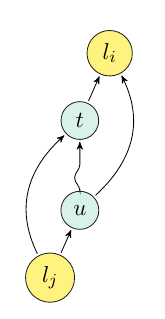
\includegraphics[]{figures/ALT.png}
    \caption{ketidaksamaan segitiga untuk ALT (diadaptasi dari~\cite{Bast2015}).}
    \label{fig:alt-triangle-ineq}
\end{figure}

Teknik akselerasi lain adalah dengan menggunakan teknik \textit{Separator-Based}. Teknik ini memanfaatkan fakta bahwa jaringan jalan dapat dibagi menjadi wilayah-wilayah yang lebih kecil dan seimbang (sel-sel) yang dipisahkan oleh sekumpulan titik simpul atau sisi, yang disebut sebagai pemisah. Teknik High-Performance Multilevel Routing (\cite{DellingHPML}) memanfaatkan \textit{vertex separators}, yaitu subset simpul-simpul $S\subset V$ yang mana penghapusannya mengurai graf menjadi beberapa sel, dan proses pembuatan partisi dilakukan secara rekursif pada setiap sel sehingga menghasilkan $multilevel \ overlay \ graph$. Fase praproses dari teknik ini dimulai dengan memilih subset $S$ lalu mempartisi graf jaringan jalan dengan menggunakan subset tersebut. Lalu, untuk setiap simpul $u,v\in S$, sebuah sisi $(u,v)$ ditambahkan ke graf \textit{overlay} $G'$ jika rute terpendek dari $u$ dan $v$ tidak mengandung simpul $w\in S$. Teknik ini juga menambahkan sisi dari simpul pemisah pada level $i$ dan simpul-simpul pemisah pada level $(i-1)$. Lihat Gambar~\ref{fig:hpml} untuk ilustrasi. Teknik HPML dapat menjawab kueri acak pada graf jaringan jalan Eropa Barat dengan 18 juta simpul dan 42.5 juta sisi dengan hitungan waktu 0.01 milidetik (\cite{Bast2015}). Teknik lain dari \textit{separator-based techniques} adalah Customizable Route Planning (CRP) (\cite{Delling2015}). Pada fase praproses, teknik ini melakukan partisi graf hingga menghasilkan graf \textit{overlay} $\mathcal{H}=(C_1,\ldots,C_k)$ dari simpul-simpul awal graf menjadi sel-sel seimbang yang menimalkan jumlah dari sisi potong (yang menghubungkan simpul-simpul batas yang terletak pada sel yang berbeda). Sisi-sisi jalan pintas yang menghubungkan antara titik-titik batas (yang merupakan rute terpendek dari setiap pasang simpul batas) dalam setiap sel ditambahkan pada graph \textit{overlay}. Lihat Gambar~\ref{fig:crp-overlay} untuk ilustrasi graf \textit{overlay} menggunakan CRP. Pada fase kustomisasi, bobot dari setiap sisi jalan pintas dihitung dengan menggunakan algoritma dijkstra yang dijalankan secara paralel pada setiap simpul batas, hal ini memungkinkan pembaruan bobot pada sisi-sisi graf menyesuaikan pembaruan kondisi lalu lintas. Algoritma kueri kemudian menjalankan algoritma Dijkstra pada subgraf yang diinduksi oleh sel yang berisi s dan t ditambah dengan graf \textit{overlay}. Teknik CRP dapat menjawab kueri acak pada graf jaringan jalan Eropa Barat dengan 18 juta simpul dan 42.5 juta sisi dengan hitungan waktu 1.65 milidetik (\cite{Delling2015}).


\begin{figure}[H]
    \centering
    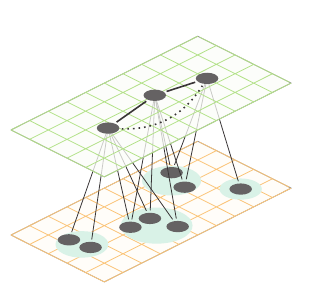
\includegraphics[]{figures/HPML.png}
    \caption{Sisi-sisi jalan pintas pada High-Performance Multilevel Routing (diadaptasi dari~\cite{Bast2015}).}
    \label{fig:hpml}
\end{figure}


\begin{figure}[H]
    \centering
    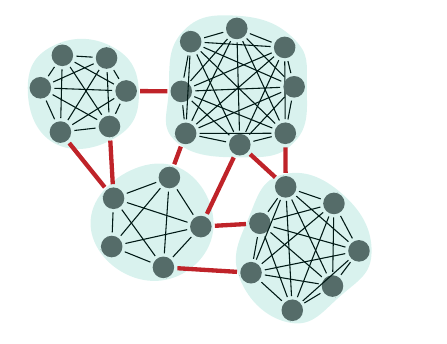
\includegraphics[]{figures/CRP.png}
    \caption{graf \textit{overlay} hasil fase kustomisasi CRP (diadaptasi dari~\cite{Bast2015}).}
    \label{fig:crp-overlay}
\end{figure}

Hierarchical techniques memanfaatkan hierarki jaringan jalan untuk mempercepat pencarian rute terpendek. Dalam jaringan jalan di dunia nyata, rute yang cukup panjang cenderung menyatu menjadi serangkaian jalan arteri yang lebih kecil, seperti jalan raya, yang berfungsi sebagai jalan utama dari perjalanan jarak jauh. Dengan memanfaatkan struktur ini, metode hierarki mengurangi ruang pencarian dengan berfokus pada simpul dan sisi dengan prioritas tinggi. Salah satu algoritma yang menggunakan teknik ini adalah \textit{Contraction Hierarchies} (CH), yang diperkenalkan pada penelitian oleh \cite{Geisberger2012}. Algoritma ini beroperasi dalam dua tahap: prapemrosesan dan kueri. Selama prapemrosesan, simpul-simpul diurutkan berdasarkan prioritasnya dan setiap simpul akan dikontraksi. Untuk mengkontraksi simpul $v$, simpul $v$ dihapus (untuk sementara) dari graf, dan sisi jalan pintas akan dibuat diantara setiap pasangan $u, w$ dari simpul yang bersebelahan dengan $v$ jika jalur terpendek dari $u$ dan $w$ unik dan mengandung simpul $v$. Pada fase kueri, pencarian dua arah dijalankan dari sumber dan target, tetapi dibatasi pada sisi yang mengarah ke simpul berperingkat lebih tinggi. Lihat Gambar~\ref{fig:query-ch} untuk ilustrasi kueri \textit{Contraction Hierarchies}. Misalkan $d_s(u)$ dan $d_t(u)$ adalah label jarak dari pencarian maju dan pencarian mundur. Oleh karena itu, di antara semua simpul $u$ yang dikunjungi oleh kedua pencarian, simpul yang meminimalkan $d_s(u)$ +  $d_t(u)$ mewakili jalur terpendek. Kueri rute terpendek dari algoritma \textit{Contraction Hierarchies} dapat dijawab dalam hitungan waktu 0.152 milidetik (\cite{Geisberger2012}). Metode hierarki lainnya adalah algoritma Reach (\cite{Gutman2004}), Reach mendefinisikan ukuran sentralitas untuk simpul berdasarkan seberapa jauh suatu simpul berada di sepanjang jalur terpendek. Misalkan $P$ adalah lintasan $s–t$ terpendek yang memuat simpul $u$. Reach $r(u,P)$ dari simpul $u$ terhadap $P$ didefinisikan sebagai $min\{dist(s,u), dist(u,t)\}$. Reach global dari simpul $u$ pada graf $G$ adalah \textit{reach} maksimum dari $u$ pada semua semua jalur terpendek yang memuat $u$. Kueri s-t algoritma reach menjalankan algoritma dijkstra, tetapi memangkas pencarian di setiap simpul $u$ yang memiliki $dist(s,u)>r(u)$ dan $dist(u,t)>r(u)$. Nilai \textit{reach} dihitung pada fase prapemrosesan dengan cara menghitung jalur terpendek untuk semua pasangan simpul. Kueri rute terpendek dari algoritma Reach dapat dijawab dalam hitungan waktu 0.152 milidetik (\cite{Bast2015}).


\begin{figure}[H]
    \centering
    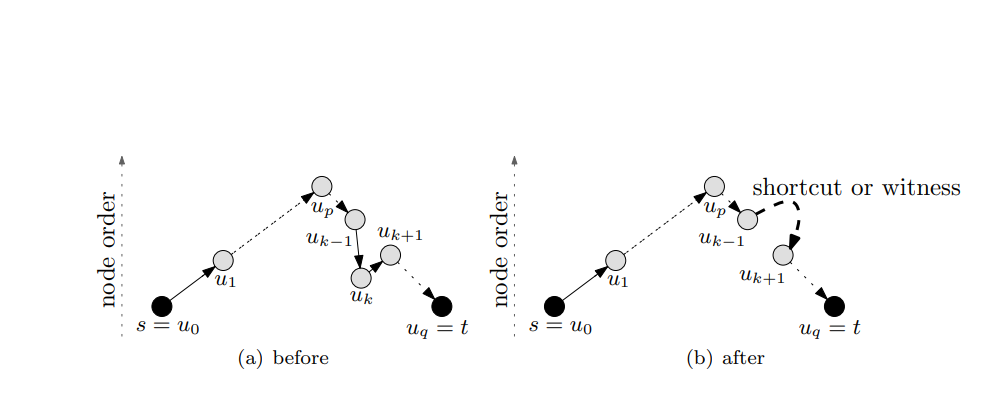
\includegraphics[width=\linewidth, keepaspectratio]{figures/CH.png}
    \caption{Ilustrasi kueri \textit{Contraction Hierarchies} (diadaptasi dari~\cite{Geisberger2012}).}
    \label{fig:query-ch}
\end{figure}


Teknik akselerasi lainnya adalah \textit{Bounded-Hop Techniques}.Ide dari teknik \textit{bounded-hop} adalah menghitung jarak antar pasangan simpul terlebih dahulu, secara implisit menambahkan "jalan pintas virtual" ke graf. Kueri kemudian dapat mengembalikan panjang jalur virtual dengan sangat sedikit \textit{hop}. Pada fase prapemrosesan, label $L(u)$ yang berisi sekumpulan simpul (\textit{hub} dari $u$) beserta jaraknya dari $u$ dihitung untuk setiap simpul $u$ pada graf, sehingga untuk setiap pasangan simpul $u,v$ jarak $dist(u,v)$ dapat ditentukan dengan melihat label $L(u)$ dan $L(v)$. pada Algoritma \textit{Hub Labelling} (HL) (\cite{Abraham2011}), \textit{hub} dari $u$ dipilih sedemikian rupa sehingga memenuhi properti \textit{cover}: untuk setiap pasang simpul $(s,t)$, $L(s)\cap L(t)$ harus memuat setidaknya satu simpul pada jalur terpendek $s-t$. Jarak dari $dist(s,t)$ dapat dihitung secara linear dengan menghitung $dist(s,t) = \min \{ dist(s,u) + dist(u,t) \mid u \in L(s) \ \text{dan} \ u \in L(t) \}$. Kueri menggunakan algoritma \textit{Hub-Labelling} dapat dijawab dalam hitungan 0.00056 milidetik. Algoritma kedua dari teknik \textit{Bounded-Hop} adalah \textit{Transit Node routing} (TNR) (\cite{Arz2013}). Ide utama dari algoritma TNR adalah memilih sejumlah simpul transit $T\subseteq V$ dan menghitung semua jarak berpasangan di antara simpul-simpul tersebut, lalu buat himpunan simpul akses $A(u)=\{v \mid v\in T \land \  v \text{ adalah adalah simpul transit pertama yang terletak pada jalur terpendek } P \text{ dari } u  \}  \subseteq T$ dari setiap simpul $u \in V \setminus T$. Pada fase kueri, algoritma ini menggunakan tabel jarak untuk memlilih rute yang meminimalkan jarak $a(s)-a(t)-t$, dimana $a(s)\in A(s) \text{ dan } a(t) \in A(t)$ adalah simpul akses. Kueri menggunakan algoritma \textit{Transit Node Routing} dapat dijawab dalam hitungan 0.00327 milidetik. Algoritma ini dapat menghasilkan hasil kueri yang tidak benar jika jalur rute terependek tidak memuat simpul dari $T$. Untuk mengatasi masalah tersebut, dibuatlah \textit{locality filter} yang memutuskan apakah kueri mengandung simpul dari $T$, jika kueri tidak mengandung simpul dari $T$ maka algoritma ini kembali menggunakan algoritma akselerasi lain seperti Contraction Hierarchies. Secara umum, teknik \textit{bounded-hop} mencapai waktu kueri yang sangat cepat (bahkan lebih cepat dibandingkan metode hierarki), tetapi dengan biaya praproses dan penggunaan memori yang relatif tinggi. Oleh karena itu, teknik ini sangat cocok untuk aplikasi navigasi statis berskala besar, namun kurang fleksibel pada skenario jaringan jalan yang sangat dinamis. Tabel~\ref{tab2:route_planning_algorithm_performance} menunjukkan performa dari beebrapa teknik akselerasi dari seribu kueri yang dihasilkan secara acak pada jaringan jalan Eropa Barat.



        \section{Map Matching dalam Jaringan Transportasi}
	\label{Map Matching dalam Jaringan Transportasi}
	Berbagai penelitian sudah dilakukan untuk menyelesaikan masalah \textit{map matching} dengan berbagai metode. Penelitian yang dilakukan oleh \cite{Krumm2009} menggunakan Hidden Markov Model untuk menghasilkan urutan segmen jalan (\textit{hidden state}) dari pengukuran GPS yang memiliki \textit{noise} (\textit{observation}. Secara formal, \textit{hidden states} dari HMM adalah $N_r$ segmen-segmen jalan, $r_ i$, $i=1,\ldots, N_r$. Untuk setiap lokasi GPS $z_t$ dalam bentuk $(longitude,latitude)$, tujuannya adalah untuk menemukan segmen jalan tempat kendaraan sebenarnya berada. Diberikan observasi $z_t$, ada probabilitas emisi untuk setiap segmen jalan $r_i$, $p(z_t\mid r_i)$, yang memberikan \textit{likelihood}. Hal ini memberikan \textit{likelihood} bahwa observasi $z_t$ akan diamati jika kendaraan benar-benar berada di ruas jalan $r_i$. Secara intuitif, \textit{states} yang lebih dekat dengan lokasi observasi memiliki probabilitas emisi yang lebih tinggi dibdandingkan dengan \textit{states} yang jauh dari observasi. Jarak antara \textit{hidden state} dengan lokasi observasi adalah \textit{measurement error} yang diasumsikan mengikuti distribusi \textit{gaussian} dengan rata-rata nol, yaitu $p(z_t \mid r_i) = \frac{1}{2\pi\sigma_z^2} 
\exp\left( -\frac{1}{2} \frac{\lVert z_t - x_{t,i} \rVert^2}{\sigma_z^2} \right)$, di mana $\lVert z_t - x_{t,i} \rVert^2$ adalah \textit{haversine distance} dari titik observasi dengan titik proyeksi observasi ke kandidat segmen jalan. Probabilitas transisi memberikan probabilitas kendaraan bergerak di antara kandidat jalan yang cocok di antara observasi $z_t$ dan $z_{t+1}$. Intuisi dari probabilitas transisi adalah ketika jarak rute (yang dihasilkan algoritma \textit{dijkstra}) antara dua titik proyeksi ke kandidat segmen lebih besar dari jarak \textit{haversine} antara dua titik observasi, maka transisi sangat tidak mungkin, namun jika selisihnya sangat kecil maka transisi pada segmen jalan tersebut cocok. Bentuk histogram dari selisih jarak rute terpendek (yang dihasilkan dari algoritma \textit{dijkstra}) dari dua titik proyeksi observasi ke kandidat segmen jalan dengan jarak \textit{haversine} antara dua titik observasi $|\lVert x_{t,i} - x_{t+1,j} \rVert_{rute} - \lVert z_{t} - z_{t+1} \rVert_{haversine} |$ sangat mirip dengan kurva distribusi eksponensial. Sehingga, probabilitas transisi dimodelkan sebagai $p(d_t)=\frac{1}{\beta}e^{\frac{-|\lVert x_{t,i} - x_{t+1,j} \rVert_{rute} - \lVert z_{t} - z_{t+1} \rVert_{haversine}  |}{\beta}}$. Tujuan utama dari HMM \textit{map matching} adalah mencari $r^{*}_{1:T} = \arg\max_{r_{1:T}} \; \log \  p(r_{1:T} \mid z_{1:T})\underset{\text{bayes}}{=} \arg\max_{r_{1:T}} \; \log  \ \pi_1({r_1}) + \log \  \ p(z_1\mid r_1)+ \sum_{t=2}^{T} \left[ \log p(r_{t-1}, r_t) + \log \ p(z_t\mid r_t) \right] $ yang mana dapat dihitung dengan efisien dengan algoritma \textit{viterbi}  (\cite{Murphy2023}). Model ini mendapatkan akurasi sebesar 98\% dengan \textit{sampling interval} 2 detik pada \textit{dataset} data mengemudi mobil yang dikumpulkan di Nagakute, Jepang. Penelitian oleh \cite{Wei2012} meningkatkan akurasi dan kecepatan pencocokan dengan memodifikasi fungsi bobot dan algoritma \textit{map-matching}. Pada paper ini, fungsi bobot yang digunakan adalah $r^{*}_{1:T} = \arg\min_{r_{1:T}} \sum_{t=2}^2 t_t\lVert z_t - x_{t,i} \rVert + \frac{2\sigma^2 |\lVert x_{t,i} - x_{t+1,j} \rVert_{rute} - \lVert z_{t} - z_{t+1} \rVert_{haversine} |}{\beta} $, di mana $t_t$ adalah interval waktu antara $z_t$ dan $z_{t+1}$. Peneliti menggunakan $\text{R}^*-\text{tree}$ mencari kandidat segmen jalan terdekat dengan radius pencarian 30 meter. Algoritma \textit{dijkstra} mengkalkulasi rute terpendek dari setiap kandidat $z_t$ ke semua kandidat dari $z_{t+1}$, dengan membatasi pencarian dari titik asal dengan radius pencarian sebesar $50m/s \times t_t$. Hasil \textit{map-matching} dengan menggunakan teknik akselerasi ini mendapatkan akurasi sebesar 98.9\% dan hanya membutuhkan waktu 1.5 detik untuk \textit{map-matching} sebanyak 14,436 titik observasi.

Metode-metode yang dijelaskan diatas hanya bisa berlaku untuk \textit{offline map-matching}, dimana kita harus memiliki seluruh data lintasan gps untuk bisa melakukan \textit{map-matching}. Namun, aplikasi navigasi membutuhkan online map matching, yaitu algoritma yang dapat memperbarui hasil \textit{map-matching} secara \textit{real-time} saat titik GPS baru tiba. Pada penelitian yang dilakukan oleh \cite{Goh2012} mengembangkan \textit{Online Hidden Markov Model} (OHMM) untuk mengatasi masalah ini. Probabilitas emisi dimodelkan sebagai Gaussian, dengan tambahan faktor setengah dari lebar jalan $w=0.5 \cdot r.w$ dan fungsi penalti kecepatan untuk membedakan jalan paralel dengan batas kecepatan berbeda. Fungsi penalti kecepatan didefinisikan sebagai $S(v_t,v_r)=\frac{v_r}{\max (0,v_t-v_r)+v_r}$, dimana $v_t$ adalah kecepatan dari observasi $t$ dan $v_r$ adalah batas kecepatan maksimum dari segmen jalan $r (r.v)$. Probabilitas emisi didefinisikan sebagai $p(t\mid r)=S(v_t,v_r) \cdot \frac{1}{2w} \int_{-w}^{w} \frac{1}{\sqrt{2\pi}\sigma_g} \exp\left( -\frac{(l - d)^2}{2\sigma_g^2} \right) \, dl.$. Untuk mendifinisikan probabilitas transisi, OHMM mendifinisikan dua fungsi skor, yaitu fungsi diskrepansi jarak $T$ dan fungsi perubahan momentum $M$. Misalkan $i,j$ adalah pasangan kandidat segmen jalan yang dikaitkan dengan dua titik observasi berurutan. Fungsi diskrepansi jarak mengukur perbedaan antara jarak tempuh  $i\rightarrow j$  yang disimpulkan sensor dan panjang lintasan $i\rightarrow j$ yang diinterpolasi. Fungsi perubahan momentum $M$ mengukur perubahan momentum rata-rata yang dialami oleh kendaraan untuk setiap segmen jalan yang diambil dalam jalur $P_{i\rightarrow j}$. OHMM menggunakan Support Vector Machine (SVM) \textit{classifier} untuk mengklasifikasikan transisi sebagai benar atau salah, menghasilkan fungsi probabilitas transisi $p(i\rightarrow j)$, di mana vektor fitur terdiri dari skor komponen yang diberikan oleh fungsi skor $T$ dan $M$. OHMM menggunakan algoritma \textit{online viterbi} dengan \textit{variable sliding window} (VSW). \textit{Sliding window} ini meluas saat titik GPS baru diterima, dan mengecil saat ditemukan convergence point pada rantai Markov—yaitu titik di mana semua jalur yang bertahan di masa depan akan berisi sub-jalur yang sama, sehingga keputusan dapat diambil tanpa menunggu titik masa depan. Eksperimen pada data bus di Singapura menunjukkan bahwa OHMM dengan VSW mencapai akurasi di atas 90\% untuk interval \textit{sampling} kurang dari 1 menit (\cite{Goh2012}). Penelitian yang dilakukan oleh \cite{Liang2016} memperkenalkan metode Online Learning Hidden Markov Model (OLMM) untuk meningkatkan akurasi \textit{map-matching} pada kondisi lalu-lintas perkotaan yang berubah-ubah tanpa perlu melakukan \textit{training ulang} dengan data berlabel. OLMM memperbarui nilai paramater $\sigma$ dari probabilitas emisi secara adaptif dengan teknik \textit{online learning}. Nilai awal $\sigma=1$ untuk paramater awal, lalu kita menyimpan $m$ hasil \textit{matching} terakhir dan menghitung ulang $\sigma$ dengan persamaan $\sigma_z=1.4826MAD(\lVert P_t-P_i\rVert_{gc})$. Untuk menghitung probabilitas transisi, pertama kita harus menghitung  matriks \textit{n-connection} $a$ , yang nilai setiap elemen baris $i$ kolom $j$ adalah jumlah lompatan yang dibutuhkan oleh segmen jalan $i$ untuk dapat sampai ke segmen jalan $j$. Probabilitas transisi dapat kita hitung dengan persamaan berikut $a_{ij}=\frac{\frac{1}{a[i][j]}}{\sum_{k}\frac{1}{a[i][k]}} \text{, jika } a[i][j] \neq 0 \text{ dan } a_{ij}=0 \text{ ,jika } a[i][j] = 0$. Definisi dari probabilitas emisi OLMM sama dengan definisi probabilitas emisi HMM (\cite{Krumm2009}). Hasil eksperimen pada data lintasan gps pada peta Seattle menunjukkan bahwa OLMM mencapai akurasi sebesar 98.57\% dan stabil ketika ukuran jendela lebih dari 15 titik observasi (\cite{Liang2016}).


Penelitian oleh \cite{Jagadeesh2017} memperluas HMM untuk data gps yang \textit{sparse} (interval \textit{sampling} sangat rendah) dengan menggabungkannya dengan \textit{route choice model} (RCM). Definisi probabilitas emisi dari penelitan ini masih sama dengan definisi probabilitas emisi pada penelitian oleh (\cite{Krumm2009}). Untuk mendefinisikan probabilitas transisi, peneliti mengusulkan ukuran dari keberlikuan untuk jalur optimal $y(s_{t-1}, s_{t,k})$ dan ketidakmungkinan temporal $z(s_{t-1}, s_{t,k})$ antara \textit{state} $s_{t-1} \text{ dan } s_{t,k}$. Ukuran keberlikuan didefinisikan dengan $y(s_{t-1}, s_{t,k})=\frac{d(s_{t-1,j}. s_{t,k})-g(s_{t-1,j},s_{t,k})}{\Delta T}$, dimana $d$ adalah jarak rute terpendek dan g adalah jarak \textit{haversine}. Ketidakmungkinan temporal digunakan untuk menyaring  jalur yang tidak dapat dilalui dalam interval waktu T kecuali kendaraan berjalan dengan kecepatan yang sangat tinggi. Ketidakmungkinan temporal didefinisikan dengan $z(s_{t-1,j}, s_{t,k})=\frac{max((f(s_{t,1,j}, s_{t,k}) - \Delta T), 0)}{\Delta T}$, dimana $f(s_{t,1,j}, s_{t,k}) $ adalah waktu tempuh tercepat antara \textit{state} $s_{t-1,j} \text{ dan } s_{t,k}$. Peneliti berasumsi distribusi dari ketidakmungkinan temporal dan ukuran keberlikuan mengikuti distribusi eksponensial. Probabilitas transisi didefinisikan dengan $P(s_{t,k}\mid s_{t-1,j})=\lambda_y e^{-\lambda_y y(s_{t-1}, s_{t,k})} \lambda_z e^{-\lambda_z z(s_{t-1}, s_{t,k})}$. Algoritma \textit{online viterbi} digunakan untuk menghasilkan lintasan parsial yang mana akan dievaluasi ulang dengan beberapa rute alternative yang dihasilkan oleh \textit{choice set generation}. Peneliti juga mendefinisikan probabilitas pilihan rute, yang memberikan probabilitas dari pengemudi memilih rute alternative $p_i$ dari himpunan rute pilihan $C$ berdasarkan model logit multinomial yang diturunkan dari data rute aktual pengemudi. Untuk setiap rute alternative dan rute yang dihasilkan algoritma \textit{online viterbi}, hitung probabilitas \textit{route choice} dan probabilitas \textit{observation generation}, rute yang dihasilkan adalah rute dengan hasil perkalian probabilitas pilihan rute dan \textit{observation generation} tertinggi. Probabilitas \textit{observation generation} adalah probabilitas bahwa data lintasan observasi gps dihasilkan saat pengemudi melintasi di sepanjang jalan pada rute alternatif. Metode gabungan \textit{Online} HMM+RCM menghasilkan akurasi 91.3\% pada data \textit{sparse} dengan interval \textit{sampling} 1-5 menit.

\cite{Huang2022} mengusulkan metode Incremental Map Matching (IMM) yang dapat mengatasi lintasan GPS dengan interval \textit{sampling} yang sangat tinggi secara \textit{real-time} dan lintasan gps dicocokan secara \textit{batch} sehingga waktu komputasi jauh lebih cepat. Algoritma ini dimulai dengan memulai dari \textit{naive matching}, yaitu mencocokan titik=titik observasi gps ke titik proyekesi pada segmen jalan terdekat. Lalu, pada setiap titik gps yang baru diproses algoritma menghitung ukuran \textit{batch} $\delta$ dengan mempertimbangkan kecepatan saat ini, kecepatan rata-rata, interval \textit{sampling}, percepatan, dan panjang segmen jalan berikutnya. Setelah menghitung ukuran \textit{batch} $\delta$, jika algoritma mendeteksi bahwa $r(p_{i+\delta}) \neq r(p_i)$ dan $r(p_{i+\delta}) \neq r(p_{i+1})$, akan dijalankan strategi \textit{voting} untuk pencocokan segmen jalan untuk semua lintasan gps $p_{i+1}\rightarrow,\ldots,\rightarrow p_{i+\delta}$. Strategi voting memilih segmen jalan dengan \textit{voting} tertinggi untuk sublintasan gps $p_{i+k}, 1\leq k \leq \delta$. Hasil dari \textit{map-matching} untuk sublintasan $p_{i+k}, 1\leq k \leq \delta$ adalah segmen jalan dari hasil strategi \textit{voting}. Metode ini mendapatkan akurasi sebesar 92\% untuk interval \textit{sampling} 1 detik. Penelitian oleh \cite{Hu2023} mampu mengkalibrasi data observasi secara adaptif dan meningkatkan akurasi dalam berbagai kondisi lalu lintas yang kompleks. Setiap titik gps baru $g^{(i)}$ tiba, algoritma menghasilkan himpunan titik kandidat dengan \textit{K Nearest Neighbors} dengan radius pencarian $r$. Hitung skor fitur kecepatan $s_u(v_m^{(i)})$, posisi  $s_z(x_m^{(i)})$, dan arah $s_\theta(\alpha_m^{(i)})$ dari titik gps $i$ dengan mempertimbangkan fitur-fitur dari setiap titik kandidat, buang titik-titik kandiddat dengan $s_u(v_m^{(i)})=0$. Lalu, hitung $score^{(i)}$, vektor bobot $\mathbf{w}^{(i)}$, dan vektor probabilitas titik-titik kandidat $\mathbf{p}^{(i)}$ dengan persamaan $\mathbf{w}^{(i)*},\mathbf{p}^{(i)*}=\arg\max_{\mathbf{w}^{(i)},\, \mathbf{p}^{(i)}} \mathbf{w}^{(i)T} \mathbf{s}^{(i)} \mathbf{p}^{(i)}$, dimana matriks $s^{(i)} \in \mathbb{R}^{3\times |C^{(i)}|}$ adalah matriks skor fitur posisi, kecepatan, dan arah dan $\mathbf{w}$ adalah vektor bobot untuk setiap fitur. Jika $score^{(i)} < \tau$, hapus titik gps $g^{(i)}$ dan hentika proses pencocokan. Setelah mendapatkan skor, hasilkan kandidat dan rute optimal yang cocok dengan persamaan $c^{(i)*}=\min_{path}(length-\eta\sum_i p_{matched}^{(i)})$. Jika titik gps saat ini dan titik gps sebelumnya dihapus, maka jalankan mekanisme koreksi retrospektif dimana algoritma melakukan koreksi kembali terhadap hasil matching sebelumnya sehingga mengurangi kesalahan detour. Hasil eksperimen pada \textit{dataset} peta Shanghai dan Singapura menunjukkan bahwa AMM mengalami peningkatan akurasi sebesar 32\% dibandingkan dengan metode HMM (\cite{Krumm2009}) pada kondisi lalu lintas yang kompleks (\cite{Hu2023}).

Meskipun metode-metode \textit{map matching} terdahulu seperti HMM dan variasinya memberikan akurasi yang tinggi, namun hasil dari pendekatan-pendekatan \textit{online map-matching} yang dijelaskan diatas adalah lintasan parsial yang sudah di cocokkan dari seluruh lintasan gps. Dengan kata lain, hasil \textit{online map-matching} mengalami keterlambatan dalam menentukan posisi kendaraan terkini. Hal ini menyebabkan metode-metode \textit{ online map matching} diatas tidak dapat memberikan respons secara \textit{real-time}, yang menjadikannya tidak cocok untuk digunakan dalam aplikasi navigasi. Hasil penelitian \textit{map-matching} yang ditinjau dapat dilihat pada tabel 2.2 yang menunjukkan perbandingna seluruh penelitian sebelumnya.




    \section{Perencanaan Rute dalam Jaringan Transportasi Bergantung Pada Waktu}
    \label{Perencanaan Rute dalam Jaringan Transportasi Bergantung Pada Waktu}
    Semua teknik akselerasi pencarian rute terpendek, seperti ALT, Arc Flags, Customizable Route Planning, Contraction Hierarchies yang dijelaskan pada subbab 2.1 beroperasi pada jaringan jalan tidak bergantung pada waktu, dimana bobot dari setiap sisi statis dan tidak bergantung pada waktu. Pada jaringan jalan perkotaan, waktu tempuh setiap jalan sering berubah karena kemacetan. Oleh karena itu, teknik akselerasi untuk jaringan jalan tidak bergantung pada waktu seringkali tidak menghasilkan rute yang optimal. Oleh karena itu beberapa penelitian mengusulkan beberapa teknik akselerasi yang dapat diterapkan pada jaringan jalan bergantung pada waktu. Pada jaringan jalan bergantung pada waktu, bobot dari setiap sisi $e$ dari graf adalah sebuah fungsi periodik $len(e,x): \Pi \rightarrow \mathbb{R}^{+}, \Pi=[0,p],p\in \mathbb{N}$. Algoritma klasik dijkstra dapat diterapkan pada jaringan jalan bergantung pada waktu dengan sedikit modifikasi (\cite{Cooke1966}). Ketika melakukan relaksasi sisi $(u,v)$ bobot dari sisi dievaluasi dengan bobot sisi untuk waktu $\tau + d(s,u,\tau)$. 

Penelitan oleh \cite{Nannicini2008} memperkenalkan algoritma ALT yang beroperasi pada jaringan jalan bergantung pada waktu. Pemilihan \textit{landmark} dan komputasi jarak antara landmarks dan semua simpul beroperasi pada graf batas bawah $\underline{G}$, dimana $\underline{G}=(V,\underline{E})=(V,\{e \mid e\in E \text{ dan } len(e, x)=\min_{x\in \Pi } len(e, x)  \})$. Fase 1 dari pencarian dua arah ALT, terdiri dari pencarian maju yang beroperasi pada graf bergantung pada waktu, dan dan pencarian mundur berjalan pada graf batas bawah $\underline{G}$. Semua simpul yang diselesaikan oleh pencarian mundur ditambahkan ke himpunan M, pencarian berhenti ketika kedua pencarian bertemu pada simpul yang sama. Fase 2 dari kueri dua arah ALT, pencarian pada fase pertama masih dapat dilanjutkan selama nilai minimum dari \textit{key} dari \textit{priority queue} pencarian mundur $\beta \leq \mu$, dimana $\mu=\ \gamma_{\tau}(p_v) \text{ dimana }\gamma_{\tau}(p_v) \text{ adalah total bobot dari rute } p_v \text{ dari } s \text{ ke }t \text{ melewati }v$. Pada fase ketiga, hanya pencarian maju yang dijalankan dan hanya simpul $v\in M$ yang boleh di kunjungi. Pencarian maju fase ketiga berhenti ketika $t$ di hapus dari \textit{priority queue}. 


Teknik akselerasi Arc-Flags yang dipekernalkan oleh \cite{Kohler2005} juga dapat diadaptasi untuk jaringan jalan bergantung pada waktu. Arc-flag $AF_C(e)$ di tetapkan nilainya true jika $e$ terletak pada jalur rute terpendek menuju suatu simpul pada sel $C$ setidaknya satu kali selama periode waktu $\Pi$. Untuk komputasi arc-flags pada graf bergantung pada waktu, buat graf profil di graf terbalik $\overleftarrow{G}$ untuk semua simpul batas $b\in B_C$ untuk semua sel $C$. Lalu, tetapkan nilai $AF_C(u,v)=true$ jika sisi $(u,v)$ merupakan $PG-edge$ dan terletak pada jalur terpendek pada setidaknya satu graf profil yang dibangun dari semua simpul batas $b\in B_C$. Kueri dilakukan dengan \textit{time-dependent} dijkstra dengan hanya melakukan relaksasi sisi $(u,v)$ yang memiliki nilai $AF_C(u,v)=true$ jika $C$ adalah sel dari simpul target. Untuk membangun profil graf $PG$, jalankan algoritma dijkstra dari simpul asal dan tetapkan label jarak $d_*(s,s)=\text{jarak antara s dan s untuk semua kemungkinan waktu keberangkatan} \in \Pi=0$ dan $d_*(s,u)=\infty$. Lalu, disetiap iterasi, simpul $u$ dengan nilai \textit{key} $\underline{d_*^{(s,u)}}$ paling kecil dihapus dari \textit{priority queue}. Lakukan relaksasi sisi $(u,v)$ jika dan hanya jika $l(v)=d_*(s,u)\oplus len(e)<d_*(s,v) , e=(u,v)$, dimana $f\oplus g=g\circ f$. Pencarian dihentikan ketika $\underline{d}(s,u)\geq \overline{d}(s,t)$. Sisi $(u,v)$ disebut sebagai $PG-edge$ jika $d_*(s,u)\oplus len(e)>d_*(s,v)$ tidak berlaku.



Metode Time-Dependent Contraction Hierarchies (TCH) yang diperkenalkan oleh \cite{Veit2013} merupakan perluasan dari Contraction Hierarchies (CH) pada graf dengan bobot bergantung waktu. Pada fase praproses, simpul-simpul diurutkan berdasarkan fungsi biaya yang dihitung melalui kontraksi simulasi dengan mempertimbangkan kedalaman hierarki, rasio jumlah sisi jalan pintas dengan sisi yang dihapus, jumlah sisi asli yang terwakili oleh sisi jalan pintas, dan kompleksitas dari fungsi waktu tempuh sisi. Simpul kemudian dikontraksi menurut urutan fungsi biaya. Untuk setiap pasangan $u\rightarrow_f x \rightarrow_f v$ akan diihtung waktu kedatangan ke $v$ dari $u$ melalui simpul $x$ $h_{u\rightarrow x \rightarrow v}=g\oplus f + \tau_0$. Jika rute $u\rightarrow_f x \rightarrow_f v$ merupakan rute \textit{earliest arrival} untuk setidaknya satu waktu keberangkatan $\tau_0$, maka ditambahkan sisi jalan pintas $u\rightarrow v$. Kueri dapat dijawab dengan cara pencarian dua arah, dimana pencarian maju menggunakan prosedur \textit{time-dependent dijkstra} dan pencarian mundur menggunakan \textit{pencarian interval profil}.



    \section{Prediksi Kecepatan Lalu Lintas}
    \label{Prediksi Kecepatan Lalu Lintas}
    Prediksi kecepatan lalu lintas merupakan komponen penting dalam sistem transportasi cerdas, karena hasil dari prediksi bisa digunakan untuk pengambilan keputusan yang lebih baik dalam perencanaan rute, navigasi \textit{real-time}, dan manajemen lalu lintas. Metode prediksi lalu lintas terbagi menjadi dua kategori, yaitu berbasis model dinamis dan metode berbasis data. Pendekatan dinamis memodelkan evolusi temporal kondisi lalu lintas dari waktu ke waktu, berdasarkan hukum fisika atau matematika yang mendasari arus lalu lintas dan melakukan simulasi perilaku lalu lintas. Namun, pendekatan ini sering kali tidak realistis karena membutuhkan daya komputasi tinggi untuk simulasi berskala besar (\cite{Vlahogianni2015}). Model statistik klasik dan pembelajaran mesin adalah contoh dari metode berbasis data. Model statistik klasik seperti ARIMA banyak digunakan untuk prediksi lalu-lintas jangka pendek, Akan tetapi, model jenis ini dibatasi oleh asumsi stasioneritas  dari \textit{time sequences} dan gagal memanfaatkan korelasi spasial antar ruas jalan, sehingga kinerjanya menjadi kurang optimal dalam melakukan prediksi lalu lintas secara akurat (\cite{AhmedCook1979}).

Penelitian oleh \cite{Wang2016} mengusulkan metode \textit{deep learning} bernama Error-feedback Recurrent Convolutional Neural Network (ECRNN). Model ini terdiri dari lima \textit{network layer}: \textit{input layer}, \textit{convolution layer}, \textit{pooling layer}, \textit{error-feedback recurrent layer}, dan \textit{output layer}. \textit{Input layer} membangun matriks \textit{spatio-temporal} yang menyimpan kecepatan lalu lintas dari setiap segmen yang terhubung secara spasial dari waktu ke waktu, yang memungkinkan model untuk mempelajari ketergantungan antar segmen secara alami. Fungsi dari \textit{convolution layer} dan \textit{pooling layer} adalah untuk mengekstrak fitur dari matriks \textit{input spatio-temporal}. \textit{Error-feedback recurrent layer} berfungsi untuk mempelajari fitur temporal dan mengkompensasi error prediksi dengan menggunakan hasil prediksi periode sebelumnya. \textit{Output layer} berfungsi untuk menghasilkan prediksi kecepatan lalu lintas. Peneliti mengevaluasi model dari data kecepatan GPS taksi yang dikumpulkan dari 202 jalan raya di kota Beijing, data gps di sampel setiap 5 menit. Peneliti membandingkan model ERCNN dengan Auto Regression Integrated Moving Average (ARIMA), Support Vector Regression (SVR), Stacked auto Encoders (SAE), dan 1D Convolutional Neural Network (1D-CNN). Model ECRNN mengungguli semua metode lainnya di semua \textit{benchmark} dengan RMSE sekitar 6\% pada panjang interval 10 menit. Namun, pada metode ECRNN \textit{convolution layer} hanya mengekstrak fitur dari segmen-segmen jalan yang terhubung dalam jangkauan 1-\textit{hop}, sehingga model tidak mempelajari fitur spasial jaringan transportasi secara optimal. Penelitian oleh \cite{Zhongjian2018} mengusulkan model Look-up Convolution Recurrent Neural Network(LC-RNN) untuk mengatasi keterbatasan model ECRNN dalam mempelajari fitur spasial. Model LC-RNN secara eksplisit mempelajari dinamika spasial dari jaringan jalan lokal melalui \textit{look-up convolution layer}. Kemudian \textit{LSTM layer} mempelajari pola ketergantungan temporal jangka panjang dari output \textit{look-up convolution layer} dengan mempertimbangkan konteks spasial sekitarnya. Selain mempelajari tren \textit{spatio-temporal}, model juga mengekstrak informasi lain seperti pola periodik (harian dan mingguan) dan faktor konteks, seperti cuaca, hari libur, dll. \textit{Fusion layer} memadukan output dari \textit{context extraction layer} \textit{peridoc layer}, dan \textit{LSTM layer} untuk menghasilkan prediksi kecapatan lalu lintas. Peneliti mengevaluasi model menggunakan Beijing \textit{trajectory dataset} dan membandingkan performanya dengan model Support Vector Regression, H-ARIMA, LSTM, SAE, Graph Convolution, ST-ResNet, dan DCNN. Pada dataset Beijing, model LC-RNN mendapatkan RMSE sebesar 4.686 mengungguli semua model yang dibandingkan. 

Beberapa penelitian terbaru menggunakan arsitektur Graph Neural Network untuk memprediksi kecepatan lalu lintas. Penelitan oleh \cite{Yu2018} mengusulkan model Spatio-Temporal Graph Convolutional Networks untuk prediksi kecepatan lalu lintas dengan memodelkan jaringan lalu lintas sebagai graf. Model STGCN terdiri dari dua blok ST-Conv dan sebuah \textit{fully-connected output layer}. Setiap blok ST-Conv terdiri dari dua Temporal Gated-Convolutional Layer dan sebuah Spatial Graph-Convolutional Layer. Spatial Graph-Convolutional Layer teridiri dari operasi \textit{graph convolutions} yang diaproksimasi degnan menggunakan \textit{Chebyshev Polynomials Approximation} orde 2 mampu mengekstrak fitur spasial yang penting. Temporal Gated-Convolutional Layer tediri dari satu Gated CNN yang merupakan 1-D Convolution dengan menggunakan fungsi aktivasi berupa Gated Linear Unit (GLU) (\cite{Gehring2017}). Peneliti mengevaluasi model STGCN dengan membandingkannya dengan Historical Average, ARIMA, LSVR, Feed-forward Neural Network, FC-LSTM, dan Graph Convolution GRU (GCGRU).  Hasil eksperimen menunjukkan bahwa model STGCN menghasilkan performa terbaik untuk semua panjang horison prediksi dengan skor RMSE sebesar 5.20 pada panjang horison prediksi 15 menit (\cite{Yu2018}). Namun, prediksi model STGCN untuk banyak \textit{time step} berikutnya sangatlah lambat karena sifat model yang \textit{autoregressive} dimana prediksi pada \textit{time step} berikutnya berdasarkan prediksi \textit{time step} sebelumnya. Penelitian oleh \cite{Wu2019} mengusulkan model Graph Wavenet untuk mengatasi masalah lambatnya waktu prediksi STGCN untuk beberapa \textit{time step}. Banyak model Graph Neural Network sebelumnya mengasumsikan struktur graf lalu lintas tetap dan diketahui, padahal hubungan spasial yang sebenarnya seringkali tidak sepenuhnya tercermin dalam adjacency matrix yang ditentukan secara eksplisit. Untuk mengatasi hal ini, Graph Wavenet memperkenalkan \textit{self-adaptive adjacency matrix} dan \textit{stacked dilated causal convolution}. \textit{Self-adaptive adjacency matrix} mempelajari ketergantungan spasial tersembunyi tanpa pengetahuan mengenai \textit{adjacency matrix} yang sebenarnya yang dipelajari melalui \textit{stochastic gradient descent}. \textit{Stacked dilated causal convolution} memungkinkan \textit{receptive field} yang membesar secara eksponensial seiring dengan kedalaman \textit{layer}, hal ini memungkinkan jaringan konvolusi untuk menangkap sekuens yang lebih panjang  dan menghemat sumber daya komputasi (\cite{Wu2019}).  Model Graph Wavenet dievaluasi pada dua dataset publik: METR-LA (207 sensor lalu lintas di Los Angeles) dan PEMS-BAY (325 sensor di Bay Area). Dalam horizon prediksi 15, 30, dan 60 menit, Graph WaveNet secara konsisten mencapai performa terbaik dibandingkan dengan model ARIMA, FC-LSTM, WaveNet, DCRNN, GGRU, dan STGCN. Sebagai contoh, pada dataset METR-LA, Graph WaveNet memperoleh  MAE 3.53, melampaui STGCN dengan MAE 4.59 dan dengan MAE DCRNN 3.60 untuk horison waktu 15 menit.

Tantangan utama dalam prediksi lalu lintas adalah kompleksitas hubungan spasial dan temporal yang saling memengaruhi antar lokasi serta keanekaragaman pola tersebut di berbagai wilayah (misalnya distrik bisnis dan perumahan memiliki pola lalu lintas yang berbeda). Sebagian besar model deep learning sebelumnya, seperti STGCN (\cite{Yu2018}) dan Graph Wavenet (\cite{Wu2019}), mengasumsikan bahwa ketergantungan spasial dan temporal bersifat seragam di seluruh node jaringan jalan. Penelitian oleh \cite{Pan2019} mengusulkan model ST-Metanet untuk mengatasi masalah ini dengan menggunakan meta-learning untuk menghasilkan parameter model berdasarkan atribut geografis tiap lokasi dan hubungan antar lokasi. Arsitektur ST-MetaNet berbasis pada Sequence-to-Sequence (Seq2Seq) yang terdiri dari \textit{encoder} dan \textit{decoder}. \textit{Encoder} berfungsi untuk mengkodekan sekuens informasi historis dari trafik $\{X_{t-\tau_{in}+1},\ldots,X_t\}$ menghasilkan \textit{hidden states} $\{H_{RNN}, H_{Meta-RNN}\}$,  yang mana digunakan sebagai input dari \textit{decoder} yang selanjutnya memprediksi sekuens $\{\hat{Y}_{t+1},\ldots, \hat{Y}_{t+\tau_{out}}\}$. Baik encoder maupun decoder memiliki tiga komponen utama: (1) Meta-Knowledge Learner (NMK dan EMK) untuk mengekstrak representasi node dan edge dari atribut geografis seperti POI, GPS, dan kepadatan jaringan jalan, (2) Meta-GAT (Meta Graph Attention Network) untuk mempelajari korelasi spasial yang beragam melalui pembuatan parameter atensi yang berbeda untuk setiap pasangan node berdasarkan meta-knowledge, dan (3) Meta-RNN untuk memodelkan korelasi temporal yang beragam dengan menghasilkan bobot GRU yang spesifik untuk tiap node, sehingga setiap lokasi memiliki model temporalnya sendiri. ST-MetaNet diuji pada prediksi kecepatan lalu lintas menggunakan data lintasan GPS taksi di Beijing . Hasil eksperimen menunjukkan bahwa ST-MetaNet secara konsisten mengungguli model-model baseline seperti ARIMA, GBRT, Seq2Seq, GAT-Seq2Seq, ST-ResNet, dan DCRNN dalam metrik MAE dan RMSE. Model ST-MetaNet mendapatkan RMSE dan MAE secara berturut-turut sebesar (7.52,3.60), sedangkan Gat-SeqSeq (8.03,3.93) dan Seq2Seq (8.88, 4.38) untuk horison waktu 15 menit.

Penelitian oleh \cite{Guo2019} mengusulkan  Attention based Spatial-Temporal Graph Convolutional Network (ASTGCN), sebuah model yang dirancang untuk meningkatkan akurasi prediksi aliran dan kecepatan lalu lintas. ASTGCN memadukan Spatial-Temporal Attention dan Graph Convolution pada dimensi temporal dan spasial, dan terstruktur menjadi tiga komponen independen untuk menangkap pola terkini, pola harian-periodik, dan pola mingguan-periodik. Input deret waktu dari ASTGCN dipecah menjadi tiga bagian, yaitu deret waktu terkni, deret waktu periode harian, dan deret waktu periode Mingguan. Masing-masing deret waktu menjadi input untuk masing masing tiga blok Spatio-Temporal. Spatial-Temporal Attention berfungsi untuk menangkap korelasi spasial dan temporal pada jaringan lalu lintas. Modul Graph Convolution yang diusulkan  terdiri dari Graph Convolution dalam dimensi spasial, menangkap ketergantungan spasial dari lingkungan dan  Graph Convolution  sepanjang dimensi temporal, mengeksploitasi ketergantungan temporal dari waktu terdekat. Keluaran dari tiga blok komponen (terkini, harian, mingguan) digabungkan melalui bobot yang dapat dipelajari untuk menghasilkan prediksi akhir, yang memungkinkan model untuk secara adaptif menekankan pola temporal yang berbeda untuk segmen jalan yang berbeda. Untuk evaluasi, ASTGCN diuji pada dua \textit{dataset}, yaitu PeMSD4  dan PeMSD8. Model ini dibandingkan dengan delapan model, yaitu HA, ARIMA, VAR, LSTM, GRU, STGCN, GLU-STGCN, dan GeoMAN.Hasilnya menunjukkan bahwa ASTGCN mencapai RMSE dan MAE terendah pada kedua set data, mengungguli semua model. Sebagai contoh, pada data PEMS4, ASTGCN mendapatkan RMSE sebesar 32,82 mengungguli STGCN dengan RMSE 38,29 dan GeoMAN dengan RMSE 37,84. Metode berbasis GCN membutuhkan pra-pendefinisian interkoneksi graf dengan ukuran jarak, graf yang dihasilkan dengan cara ini mungkin mengandung bias dan tidak dapat diadaptasi ke domain tanpa pengetahuan mengenai jaringan jalan dari graf. Penelitian oleh \cite{Bai2020} mengusulkan model Adaptive Graph Convolutional Recurrent Network (AGCRN) yang dirancang untuk memodelkan ketergantungan spasial dan temporal tanpa bergantung pada graf yang sudah ditentukan sebelumnya. AGCRN terdiri dari dua modul: (1) modul Node Adaptive Parameter Learning (NAPL) untuk mempelajari pola spesifik dari simpul graf untuk setiap deret waktu, modul NAPL memfaktorkan parameter GCN ke dalam \textit{weights pool} dan \textit{bias pool}, yang memungkinkan setiap node lalu lintas memiliki parameter spesifiknya sendiri; (2) modul Data Adaptive Graph Generation (DAGG) untuk mempelajari \textit{node embedding } dari data dan menghasilkan graf secara adaptif selama pelatihan (\cite{Bai2020}). Peneliti menguji AGCRN pada \textit{dataset} PEMSD4 dan PEMSD8 dengan metrik MAE,RMSE, dan MAPE. Peneliti juga membandingkan AGCRN dengan baseline yang banyak digunakan dan beberapa model terbaik untuk prediksi kecepatan lalu lintas. Pada PEMSD8, AGCRN mendapatkan peingkatan sebesar 4-7\% terhadap model terbaik sebelumnya di seluruh metrik dan peningkatan sebesar 3-5\% untuk \textit{dataset} PEMSD4. Detail lengkap dari setiap dataset, metode, dan hasil penelitian yang ditinjau dapat dilihat pada tabel 2.3 yang menunjukkan perbandingan seluruh penelitian sebelumnya.



    \section{Perangkat Lunak Route Planning Sumber Terbuka Untuk Openstreetmap}
    \label{Perangkat Lunak Route Planning Sumber Terbuka}
    Berbagai algoritma pencarian rute terpendek dan teknik akselerasi yang telah dijelaskan banyak digunakan pada perangkat lunak perencanaan rute (route planning) sumber terbuka berbasis OpenStreetMap (OSM). Berbagai perangkat lunak ini menggunakan data jaringan jalan OSM untuk menyediakan layanan navigasi serta pencarian rute secara efisien. Beberapa contoh perangkat lunak perencanaan rute sumber terbuka yang populer antara lain GraphHopper, OSRM (Open Source Routing Machine), dan Valhalla. Graphopper (\cite{Graphopper}) menggunakan algoritma Contraction Hierarchies untuk pencarian rute terpendek . Perangkat lunak OSRM (\cite{Luxen2011}) menggunakan algoritma Time-Independent Customizable Route Planning untuk pencarian rute terpendek. Valhalla (\cite{Valhalla}) menggunakan algoritma $A*$ dengan menggunakan teknik akselerasi yang mirip dengan Customizable Route Planning, yaitu dengan menambahkan sisi jalan pintas pada subgraf yang terdiri dari jalan raya dan jalan arteri. Ketiga perangkat lunak diatas menggunakan metode Hidden Markov Model (\cite{Newson2009}) untuk penyelesaian masalah \textit{offline map matching}. Meskipun ketiga perangkat lunak diatas telah banyak digunakan dan mendukung fitur pencarian rute terpendek secara efisien, ketiganya belum mendukung fitur \textit{time-dependent route planning}, \textit{online map-matching}, dan prediksi kecepatan lalu lintas. Oleh karena itu, diperlukan pembuatan sebuah perangkat lunak mengintegrasikan tiga fitur tersebut, guna menghasilkan layanan navigasi yang lebih adaptif, efisien, dan akurat.


\begin{table}[h]
\setlength{\tabcolsep}{6pt}
\caption{Perbandingan performa berbagai algoritma perutean dalam hal prapemrosesan dan kinerja kueri.}
\label{tab2:route_planning_algorithm_performance}
\resizebox{\textwidth}{!}{%
\begin{tabular}{l c c c c c c}
\hline
 &  & \multicolumn{2}{c}{\textbf{Struktur Data}}  & \textbf{Kustomisasi} & \multicolumn{2}{c}{\textbf{KUERI}} \\
\cline{3-5}
\textbf{algoritma}  & & \textbf{ruang [GiB]} & \textbf{waktu [h:m]} & waktu [s] & \textbf{simpul terpindai} & \textbf{waktu [\(\mu\)s]} \\
\hline
Dijkstra     & & 0.4   & --   & -- & 9\,326\,696 & 2\,195\,080 \\
CRP          & & 0.9   & 1:00 & 1.04s  & 2\,766      & 1\,650 \\
Arc Flags    & &  0.6   & 2:46 & -- & 2\,646      & 408 \\
CH          & &  0.4   & 0:05 & -- & 280        & 110 \\
HPML         & &  1.8   & 0:50 & -- & --         & 2.55 \\
TNR         & &  2.5   & 0:22 & -- & --         & 2.09 \\
HL         & &  18.8  & 3:07 & -- & --         & 0.56 \\
\hline
\end{tabular}
} % end resizebox
\end{table}


\begin{table}[h]
\centering
\setlength{\tabcolsep}{6pt}
\caption{Perbandingan performa berbagai algoritma map-matching.}
\label{tab2:map_matching_performance}
\begin{tabular}{l l c }
\hline
\textbf{algoritma} & \textbf{dataset} & \textbf{akurasi} \\
\hline
Offline-HMM  & Seattle & 98\%   \\
FastViterbi-HMM & Seattle & 98.9\% \\
OHMM & Singapore & 92.1\% \\
OLMM & Seattle & 98.57\% \\
HMM+RCM & Singapore & 91.3\% \\
IMM & Singapore & 92\% \\
AMM & Singapore & 98.92\% \\
\hline
\end{tabular}
\end{table}

\newpage

\begin{longtable}{|p{3.75cm}|p{3.15cm}|l|l|}
\caption{Perbandingan metode prediksi kecepatan lalu lintas.}  
\label{tab2:traffic_speed_forecasting} \\
\hline
\textbf{Penulis} & \textbf{Dataset} & \textbf{Metode} & \textbf{Hasil} \\ 
\hline

\multirow{2}{*}{\cite{Wang2016}}
& \multirow{2}{*}{\shortstack{Beijing GPS \\ \textit{Trajectory}\\(horison 50 menit)}}
& ARIMA & \shortstack{ MAE: 10.0,\\ RMSE: 12.5} \\
\cline{3-4} 
 &  & SVR &  \shortstack{MAE: 10.1,\\ RMSE: 15.1} \\ 
 \cline{3-4} 
 &  & SAE & \shortstack{ MAE: 7.6,\\ RMSE: 10.0} \\ 
 \cline{3-4} 
 &  & 1D-CNN &  \shortstack{MAE:7.7,\\ RMSE: 10.0} \\
 \cline{3-4} 
 &  & CNN & \shortstack{ MAE: 7.0,\\ RMSE: 8.0} \\ 
 \cline{3-4} 
 &  & eRCNN &  \shortstack{MAE: 6.9,\\ RMSE: 7.8 } \\ 
\cline{3-4} 
\hline

\multirow{2}{*}{\cite{Zhongjian2018}}
& \multirow{2}{*}{\shortstack{Beijing GPS \\ \textit{Trajectory} \\(horison 10 menit)}} 
& ARIMA &   RMSE: 10.245 \\
\cline{3-4} 
 &  & H-ARIMA &  RMSE: 11.867 \\ 
 \cline{3-4} 
 &  & SAE & RMSE: 8.471 \\ 
 \cline{3-4} 
 &  & LSTM & RMSE: 5.958 \\
 \cline{3-4} 
 &  & DCNN & RMSE: 6.085 \\ 
 \cline{3-4} 
 &  & GC & RMSE: 5.514 \\ 
\cline{3-4} 
 &  & ST-ResNet & RMSE: 5.749 \\ 
\cline{3-4} 
 &  & LC-RNN & RMSE: 5.274 \\ 
\cline{3-4} 
\hline

\multirow{2}{*}{\cite{Yu2018}}
& \multirow{2}{*}{\shortstack{PeMSD7(L)\\(horison 45 menit)}}
& HA &  \shortstack{MAE: 4.60,\\ RMSE: 8.05} \\
\cline{3-4} 
 &  & LSVR &  \shortstack{MAE: 4.79,\\ RMSE: 8.72} \\
\cline{3-4} 
 &  & ARIMA &   \shortstack{MAE: 6.30,\\ RMSE: 9.39} \\
\cline{3-4} 
 &  & FNN &   \shortstack{MAE: 4.78,\\ RMSE: 8.46} \\ 
 \cline{3-4} 
 &  & FC-LSTM &  \shortstack{MAE: 4.66,\\ RMSE: 8.20}  \\ 
 \cline{3-4} 
 &  & GCGRU &  \shortstack{MAE: 4.12,\\ RMSE: 7.49} \\
 \cline{3-4} 
 &  & STGCN(Cheb) &  \shortstack{MAE: 3.97,\\ RMSE: 7.45} \\ 
 \cline{3-4} 
 &  & $STGCN(1^{st})$ &  \shortstack{MAE: 4.01,\\ RMSE: 7.81} \\ 
\cline{3-4}
\hline

\pagebreak
\multirow{2}{*}{\cite{Wu2019}}
& \multirow{2}{*}{\shortstack{PeMS-BAY\\(horison 60 menit)}}
& ARIMA &  \shortstack{MAE: 3.38,\\ RMSE: 6.50} \\
\cline{3-4} 
 &  & FC-LSTM &  \shortstack{MAE: 2.37,\\ RMSE: 4.96} \\
\cline{3-4} 
 &  & WaveNet &  \shortstack{ MAE: 2.35,\\ RMSE: 5.43} \\
\cline{3-4} 
 &  & DCRNN &   \shortstack{MAE: 2.07,\\ RMSE: 4.74} \\ 
 \cline{3-4} 
 &  & STGCN &  \shortstack{MAE: 2.49,\\ RMSE: 5.69} \\ 
 \cline{3-4} 
 &  & Graph Wavenet &  \shortstack{MAE: 1.95,\\ RMSE: 4.52} \\
 \cline{3-4} 
\hline


\multirow{2}{*}{\cite{Pan2019}}
& \multirow{2}{*}{\shortstack{METR-LA\\(horison 60 menit)}}
& HA &  \shortstack{MAE: 26.2,\\ RMSE: 56.5} \\
\cline{3-4} 
 &  & ARIMA &  \shortstack{MAE: 27.1,\\ RMSE: 58.3} \\
\cline{3-4} 
 &  & GBRT &   \shortstack{MAE: 22.3,\\ RMSE: 47.7} \\
\cline{3-4} 
 &  & Seq2Seq &   \shortstack{MAE: 17.8,\\ RMSE: 35.1} \\ 
 \cline{3-4} 
 &  & GAT-SeqSeq &  \shortstack{MAE: 16.3,\\ RMSE: 31.9}  \\ 
 \cline{3-4} 
  &  & ST-ResNet &  \shortstack{MAE: 16.8,\\ RMSE: 31.9}  \\ 
 \cline{3-4} 
 &  & ST-MetaNet &  \shortstack{MAE: 15.0,\\ RMSE: 29.9} \\
 \cline{3-4} 
\hline


\multirow{2}{*}{\cite{Guo2019}}
& \multirow{2}{*}{\shortstack{PeMSD8\\(horison 60 menit)}}
& HA &  \shortstack{MAE: 29.52,\\ RMSE: 44.03} \\
\cline{3-4} 
 &  & ARIMA &  \shortstack{MAE: 24.04,\\ RMSE: 43.30} \\
\cline{3-4} 
 &  & VAR &   \shortstack{MAE: 21.41,\\ RMSE: 31.21} \\
\cline{3-4} 
 &  & LSTM &   \shortstack{MAE: 23.18,\\ RMSE: 36.96} \\ 
 \cline{3-4} 
 &  & GRU &  \shortstack{MAE: 22.20,\\ RMSE: 35.95}  \\ 
 \cline{3-4} 
  &  & STGCN &  \shortstack{MAE: 18.88,\\ RMSE: 27.87}  \\ 
 \cline{3-4} 
 &  & GLU-STGCN &  \shortstack{MAE: 20.99,\\ RMSE: 30.78} \\
 \cline{3-4} 
&  & GeoMAN &  \shortstack{MAE: 17.84,\\ RMSE: 28.91} \\
 \cline{3-4} 
&  & ASTGCN &  \shortstack{MAE: 16.63,\\ RMSE: 25.27} \\
 \cline{3-4} 
\hline

\pagebreak
\multirow{2}{*}{\cite{Bai2020}}
& \multirow{2}{*}{\shortstack{PeMSD8\\(horison 60 menit)}}
& HA &  \shortstack{MAE: 34.86,\\ RMSE: 52.04} \\
\cline{3-4} 
 &  & VAR &  \shortstack{MAE: 19.19,\\ RMSE: 29.81} \\
\cline{3-4} 
 &  & GRU-ED &   \shortstack{MAE: 22.00,\\ RMSE: 36.23} \\
\cline{3-4} 
 &  & DSANet &   \shortstack{MAE: 17.14,\\ RMSE: 26.96} \\ 
 \cline{3-4} 
 &  & DCRNN &  \shortstack{MAE: 16.82,\\ RMSE: 26.36}  \\ 
 \cline{3-4} 
  &  & STGCN &  \shortstack{MAE: 17.50,\\ RMSE: 27.09}  \\ 
 \cline{3-4} 
 &  & ASTGCN &  \shortstack{MAE: 18.25,\\ RMSE: 28.06} \\
 \cline{3-4} 
&  & STSGCN &  \shortstack{MAE: 17.13,\\ RMSE: 26.86} \\
 \cline{3-4} 
&  & AGCRN &  \shortstack{MAE: 15.95,\\ RMSE: 25.22} \\
 \cline{3-4} 
\hline

\end{longtable}




\begin{table}[h]
\setlength{\tabcolsep}{6pt}
\caption{Perbandingan performa berbagai algoritma perutean dalam hal prapemrosesan dan kinerja kueri.}
\label{tab2:route_planning_algorithm_performance}
\begin{tabular}{l c c c c c}
\hline
 &  & \multicolumn{2}{c}{\textbf{Struktur Data}} & \multicolumn{2}{c}{\textbf{KUERI}} \\
\cline{3-5}
\textbf{algoritma} & \textbf{ruang [GiB]} & \textbf{waktu [h:m]} & \textbf{simpul terpindai} & \textbf{waktu [\(\mu\)s]} \\
\hline
Dijkstra      & 0.4   & --     & 9\,326\,696 & 2\,195\,080 \\
CRP           & 0.9   & 1:00   & 2\,766      & 1\,650 \\
Arc Flags     & 0.6   & 2:46   & 2\,646      & 408 \\
CH            & 0.4   & 0:05   & 280        & 110 \\
HPML          & 1.8   & 0:50   & --         & 2.55 \\
TNR           & 2.5   & 0:22   & --         & 2.09 \\
HL            & 18.8  & 3:07   & --         & 0.56 \\
\hline
\end{tabular}
\end{table}


\begin{table}[h]
\setlength{\tabcolsep}{6pt}
\caption{Perbandingan performa berbagai algoritma map-matching.}
\label{tab2:map_matching_performance}
\begin{tabular}{l l c }
\hline
\textbf{algoritma} & \textbf{dataset} & \textbf{akurasi} \\
\hline
Offline-HMM  & Seattle & 98\%   \\
FastViterbi-HMM & Seattle & 98.9\% \\
OHMM & Singapore & 92.1\% \\
OLMM & Seattle & 98.57\% \\
HMM+RCM & Singapore & 91.3\% \\
IMM & Singapore & 92\% \\
AMM & Singapore & 98.92\% \\
\hline
\end{tabular}
\end{table}

\begin{longtable}{|p{3.8cm}|p{3.8cm}|l|l|}
\caption{Perbandingan metode prediksi kecepatan lalu lintas.} \\ 
\hline
\textbf{Penulis} & \textbf{Dataset} & \textbf{Metode} & \textbf{Hasil} \\ 
\hline


\multirow{2}{*}{\cite{Wang2016}}
& \multirow{2}{*}{\shortstack{Beijing GPS \\ \textit{Trajectory}\\(horison 50 menit)}}
& ARIMA &  MAE: 10.0, RMSE: 12.5 \\
\cline{3-4} 
 &  & SVR &  MAE: 10.1, RMSE: 15.1 \\ 
 \cline{3-4} 
 &  & SAE &  MAE: 7.6, RMSE: 10.0 \\ 
 \cline{3-4} 
 &  & 1D-CNN &  MAE:7.7, RMSE: 10.0 \\
 \cline{3-4} 
 &  & CNN &  MAE: 7.0, RMSE: 8.0 \\ 
 \cline{3-4} 
 &  & eRCNN &  MAE: 6.9, RMSE: 7.8  \\ 
\cline{3-4} 
\hline

\multirow{2}{*}{\cite{Zhongjian2018}}
& \multirow{2}{*}{\shortstack{Beijing GPS \\ \textit{Trajectory} \\(horison 10 menit)}} 
& ARIMA &   RMSE: 10.245 \\
\cline{3-4} 
 &  & H-ARIMA &  RMSE: 11.867 \\ 
 \cline{3-4} 
 &  & SAE & RMSE: 8.471 \\ 
 \cline{3-4} 
 &  & LSTM & RMSE: 5.958 \\
 \cline{3-4} 
 &  & DCNN & RMSE: 6.085 \\ 
 \cline{3-4} 
 &  & GC & RMSE: 5.514 \\ 
\cline{3-4} 
 &  & ST-ResNet & RMSE: 5.749 \\ 
\cline{3-4} 
 &  & LC-RNN & RMSE: 5.274 \\ 
\cline{3-4} 
\hline

\multirow{2}{*}{\cite{Yu2018}}
& \multirow{2}{*}{\shortstack{PeMSD7(L)\\(horison 45 menit)}}
& HA & MAE: 4.60, RMSE: 8.05 \\
\cline{3-4} 
 &  & LSVR & MAE: 4.79, RMSE: 8.72 \\
\cline{3-4} 
 &  & ARIMA &  MAE: 6.30, RMSE: 9.39 \\
\cline{3-4} 
 &  & FNN &  MAE: 4.78, RMSE: 8.46 \\ 
 \cline{3-4} 
 &  & FC-LSTM & MAE: 4.66, RMSE: 8.20  \\ 
 \cline{3-4} 
 &  & GCGRU & MAE: 4.12, RMSE: 7.49 \\
 \cline{3-4} 
 &  & STGCN(Cheb) & MAE: 3.97, RMSE: 7.45 \\ 
 \cline{3-4} 
 &  & $STGCN(1^{st})$ & MAE: 4.01, RMSE: 7.81 \\ 
\cline{3-4}
\hline

\multirow{2}{*}{\cite{Wu2019}}
& \multirow{2}{*}{\shortstack{PeMS-BAY\\(horison 60 menit)}}
& ARIMA & MAE: 3.38, RMSE: 6.50 \\
\cline{3-4} 
 &  & FC-LSTM & MAE: 2.37, RMSE: 4.96 \\
\cline{3-4} 
 &  & WaveNet &  MAE: 2.35, RMSE: 5.43 \\
\cline{3-4} 
 &  & DCRNN &  MAE: 2.07, RMSE: 4.74 \\ 
 \cline{3-4} 
 &  & STGCN & MAE: 2.49, RMSE: 5.69  \\ 
 \cline{3-4} 
 &  & Graph Wavenet & MAE: 1.95, RMSE: 4.52 \\
 \cline{3-4} 
\hline


\multirow{2}{*}{\cite{Pan2019}}
& \multirow{2}{*}{\shortstack{METR-LA\\(horison 60 menit)}}
& HA & MAE: 26.2, RMSE: 56.5 \\
\cline{3-4} 
 &  & ARIMA & MAE: 27.1, RMSE: 58.3 \\
\cline{3-4} 
 &  & GBRT &  MAE: 22.3, RMSE: 47.7 \\
\cline{3-4} 
 &  & Seq2Seq &  MAE: 17.8, RMSE: 35.1 \\ 
 \cline{3-4} 
 &  & GAT-SeqSeq & MAE: 16.3, RMSE: 31.9  \\ 
 \cline{3-4} 
  &  & ST-ResNet & MAE: 16.8, RMSE: 31.9  \\ 
 \cline{3-4} 
 &  & ST-MetaNet & MAE: 15.0, RMSE: 29.9 \\
 \cline{3-4} 
\hline


\multirow{2}{*}{\cite{Guo2019}}
& \multirow{2}{*}{\shortstack{PeMSD8\\(horison 60 menit)}}
& HA & MAE: 29.52, RMSE: 44.03 \\
\cline{3-4} 
 &  & ARIMA & MAE: 24.04, RMSE: 43.30 \\
\cline{3-4} 
 &  & VAR &  MAE: 21.41, RMSE: 31.21 \\
\cline{3-4} 
 &  & LSTM &  MAE: 23.18, RMSE: 36.96 \\ 
 \cline{3-4} 
 &  & GRU & MAE: 22.20, RMSE: 35.95  \\ 
 \cline{3-4} 
  &  & STGCN & MAE: 18.88, RMSE: 27.87  \\ 
 \cline{3-4} 
 &  & GLU-STGCN & MAE: 20.99, RMSE: 30.78 \\
 \cline{3-4} 
&  & GeoMAN & MAE: 17.84, RMSE: 28.91 \\
 \cline{3-4} 
&  & ASTGCN & MAE: 16.63, RMSE: 25.27 \\
 \cline{3-4} 
\hline

\multirow{2}{*}{\cite{Bai2020}}
& \multirow{2}{*}{\shortstack{PeMSD8\\(horison 60 menit)}}
& HA & MAE: 34.86, RMSE: 52.04 \\
\cline{3-4} 
 &  & VAR & MAE: 19.19, RMSE: 29.81 \\
\cline{3-4} 
 &  & GRU-ED &  MAE: 22.00, RMSE: 36.23 \\
\cline{3-4} 
 &  & DSANet &  MAE: 17.14, RMSE: 26.96 \\ 
 \cline{3-4} 
 &  & DCRNN & MAE: 16.82, RMSE: 26.36  \\ 
 \cline{3-4} 
  &  & STGCN & MAE: 17.50, RMSE: 27.09  \\ 
 \cline{3-4} 
 &  & ASTGCN & MAE: 18.25, RMSE: 28.06 \\
 \cline{3-4} 
&  & STSGCN & MAE: 17.13, RMSE: 26.86 \\
 \cline{3-4} 
&  & AGCRN & MAE: 15.95, RMSE: 25.22 \\
 \cline{3-4} 
\hline

\end{longtable}




%-----------------------------------------------------------------
% Akhir BAB 2
%-----------------------------------------------------------------


%-----------------------------------------------------------------
% Awal BAB 3
%-----------------------------------------------------------------
\chapter{DASAR TEORI}
\label{DASAR TEORI}

	\section{Time Dependent Customizable Route Planning}
	\label{time dependent customizable route planning}
	\subsection{Pendahuluan}
\label{subsec:tdcrp-preliminaries}
Diberikan sebuah graf $G=(V,A)$, dengan setiap sisi $(v,w)\in A$ memiliki fungsi biaya nonnegatif $\ell(v,w)$. Karena graf merepresentasikan sebuah jaringan jalan, simpul merepresentasikan persimpangan dan sisi merepresentasikan segmen jalan pada jaringan jalan, dan fungsi biaya dihitung berdasarkan karakteristik segmen jalan (misalnya, waktu tempuh). Sebuah lintasan $P=(v_0,\ldots,v_k)$ adalah sebuah rangkaian simpul-simpul dengan $(v_i, v_{i+1}\in A)$, dan biayanya didefinisikan sebagai $\ell(P)=\sum_{i=0}^{k-1}\ell(v_i,v_{i+1})$. Tugas dari Time-Dependent Customizable Route Planning adalah menghitung  jalur terpendek dari suatu simpul asal $s$ ke simpul target $t$. Diberikan simpul asal $s$ dan simpul target $t$, penulis harus menghitung jarak $dist(s,t)$, yang didefinisikan sebagai $\ell(Opt)$ dari jalur terpendek lintasan $Opt$ pada graf $G$ dari $s$ ke $t$.

Sebuah partisi dari simpul-simpul $V$ adalah sebuah himpunan sel-sel $\mathcal{C}=\{C_0,\ldots, C_k\}, C_i\subseteq V$ dengan setiap simpul $v\in V$ terkandung didalam satu sel $C_i$. Misalkan $U$ adalah jumlah simpul dari sel terbesar. Partisi \textit{multilevel} dari $V$ adalah himpunan partisi $\{\mathcal{C}^{0},\ldots, \mathcal{C}^{L}\}$, dimana $l$ adalah \textit{level} dari partisi $\mathcal{C}^{l}$ dan $U^{l}$ merepresentasikan ukuran dari sel terbesar pada level $l$. $L$ adalah jumlah level dari  partisi \textit{multilevel}. $U^{0}=1$ atau dengan kata lain $U^{0}$ adalah $singleton$. Penulis juga menetapkan $\mathcal{C}^{L+1}=V$ untuk menandakan partisi pada level $L+1$ adalah graf orisinil. Untuk setiap level $l\leq L$ dan untuk setiap sel $C_{i}^{l}\in\mathcal{C}^l$, terdapat sebuah sel $C_{j}^{l+1}\in\mathcal{C}^{l+1} \text{ disebut sebagai \textit{supercell} dari } C_i^l$ dengan $C_i^l\subseteq C_j^{l+1}$. $c_l(v)$ adalah sel yang berisi simpul $v$ pada level $l$. Pada setiap level $l$ terdapat sisi batas dengan $endpoints$ terdapat pada sel yang berbeda pada level-$l$. Simpul batas pada level $l$ adalah simpul dengan setidaknya memiliki satu tetangga yang berada pada sel lain pada level $l$.  Untuk partisi \textit{multilevel}, sisi batas pada level $l$ juga merupakan sisi batas pada level dibawah $l$.

Dalam Time Dependent Customizable Route Planning, setiap sisi $a$ memiliki bobot berupa \textit{travel-time function} (TTF) $f_a:\Pi\rightarrow \mathbb{R}^{+}$, memetakan waktu keberangkatan ke waktu tempuh. Semua \textit{travel-time function} adalah \textit{continuous piecewiese linear function} dengan periode $\pi$ dan memiliki rentang nilai $\Pi=[0,\pi]$. Diberikan sebuah fungsi $f$, jumlah \textit{breakpoints} dari $f$ adalah $\mid f\mid $. Nilai maksimum dari $f$ didefinisikan dengan $f^{max}=\max_{\tau\in\Pi}f(\tau)$ dan nilai minimum dari $f$ didefinisikan dengan $f^{min}=\min_{\tau\in\Pi}f(\tau)$. \textit{Travel-time function} memenuhi sifat \textit{FIFO}, yaitu untuk bilangan riil positif sembarang $\sigma\leq\tau\in\Pi$, kondisi $\sigma+f(\sigma)\leq \tau+f(\tau)$ harus berlaku. Operasi \textit{link} didefinisikan dengan $link(f,g)=f+g \ \circ \ (identity+f)$. Operasi \textit{merge} didefinisikan dengan $merge(f,g)=min(f,g)$. Kedua operasi tersebut memiliki kompleksitas waktu $O(\mid f\mid +\mid g\mid )$. Diberikan rute $P=[v_1,\ldots,v_k]$, \textit{travel-time profile} (TTP) didefinisikan dengan $f_P:\Pi\rightarrow \mathbb{R}^{+}$, yang memetakan waktu keberangkatan $\tau$ (pada $v_1$) ke \textit{travel time} pada $P$ untuk menuju ke $v_k$. \textit{Arrival time function} $arr f:\tau\rightarrow f(\tau)+\tau$, memetakan waktu keberangkatan $\tau$ ke waktu kedatangan setelah melintasi sisi yang memiliki TTF $f$. 

Diberikan waktu keberangkatan $\tau$ dan simpul asal $s$ dan simpul target $t$, kueri \textit{earliest-arrival} (EA) menanyakan waktu tempuh minimum dari $s$ ke $t$ ketika berangkat pada waktu $\tau$. Kueri \textit{latest-departure} (LD) menanyakan waktu tempuh minimum yang mencapai simpul $t$ pada waktu $\tau$. Kueri profil menanyakan waktu tempuh minimum pada setiap kemungkinan waktu keberangkatan $\tau$, yaitu profil $f_{s,t}$ dari $s$ ke $t$. Kueri EA dapat ditangani dengan algoritma Time-Dependent Dijkstra yang pseudocodenya diberikan oleh algoritma~\ref{alg:td-dijkstra}. Kueri profile dapat ditangani dengan algoritma ProfileSearch yang pseudocodenya diberkan oleh algoritma~\ref{alg:profileSearch}

\subsection{Fase Prapemrosesan}
\label{subsec:tdcrp-preprocessing}
Pada tahapan prapemrosesan, penulis membuat partisi \textit{multilevel} dari graf jaringan jalan, lalu membuat topologi dari graf \textit{overlay}, dan membuat beberapa struktur data baru. Untuk membuat partisi multilevel, penulis menjalankan algoritma Inertial Flow \cite{Schild2015}, pada graf input untuk mnghasilkan partisi level-$L$ (dengan ukuran sel maksimum $U_1,\ldots, U_{L}$ dari atas ke bawah. Pertama-tama, penulis menjalankan Inertial Flow dengan parameter $U_L$ untuk mendapatkan sel level tertinggi. Lalu, sel-sel pada lavel dibawahnya didapatkan dengan menjalankan Inertial Flow pada masing-masing sel dari level diatasnya secara paralel. Lihat Gambar~\ref{fig:mlp-inertial-flow}. Setiap sel $C$ pada level 1 atau lebih tinggi diberi ID sekuensial unik di dalam superselnya. Dengan kata lain, di setiap supersel, subsel-subsel partisi dari supersel memiliki id sekuensial dari 0 hingga jumlah sel partisi dari supersel. Untuk setiap simpul $v$ penulis menyimpan ID dari sel dari simpul untuk setiap level dengan \textit{integer} 64-bit $PV(v)$, dimana bit yang lebih rendah merepresentasikan sel dari simpul di level yang lebih rendah. Hal ini bisa dicapai dengan cara: untuk setiap level dari sel simpul $v$, penulis mengalokasikan sejumlah $\lceil \log_2(\text{jumlah sel pada level } l) \rceil$-bit pada $PV(v)$ untuk menyimpan ID sel dari simpul $v$ pada level $l$. Penulis juga membuat matriks \textit{turnTables} $T_u$ untuk semua $u\in V$, dimana $T_u[i,j]$ merepresentasikan biaya untuk berbelok dari sisi masuk ke-$i$ dan sisi keluar ke-$j$ dari simpul $u$. Biaya untuk berbelok dari sisi masuk ke-$i$ dan sisi keluar ke-$j$ dari simpul $u$ bisa ditentukan oleh pengguna dan biasanya biaya ditentukan berdasarkan tipe belokan (contoh, \textit{u turn},  \textit{right turn}, \textit{left turn}). Untuk setiap sisi keluar $(v,w)$, penulis menyimpan \textit{head order} titik \textit{entry}(posisi dari sisi relatif terhadap sisi masuk $w$) dan \textit{head point} (simpul $w$). Untuk setiap sisi masuk $(v,w)$, penulis menyimpan \textit{tail order}/titik \textit{exit}(posisi dari sisi relatif terhadap sisi keluar $v$) dan \textit{tail point} (simpul $v$). Lihat gambar~\ref{fig:crp-exit-entry-point} untuk ilustrasi mengenai titik \textit{entry}/\textit{exit}.

\begin{figure}[h]
    \centering

    \begin{subfigure}[b]{0.45\textwidth}
        \centering
        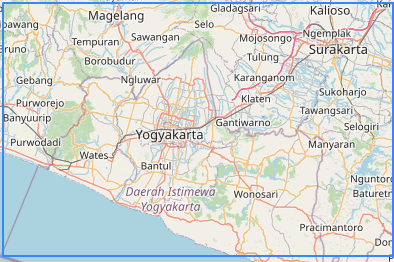
\includegraphics[width=\linewidth]{figures/original_road_networks.png}
        \caption{Graf jaringan jalan untuk peta Openstreetmap wilayah Surakarta, Daerah Istimewa Yogyakarta, dan Klaten}
        \label{fig:a}
    \end{subfigure}
    \hfill
    \begin{subfigure}[b]{0.45\textwidth}
        \centering
        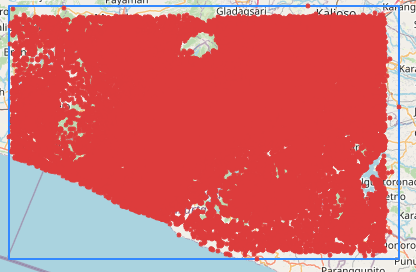
\includegraphics[width=\linewidth]{figures/partition_level_5.png}
        \caption{Partisi level 5 dengan ukuran $U_5=2^{20}$}
        \label{fig:b}
    \end{subfigure}

    \begin{subfigure}[b]{0.45\textwidth}
        \centering
        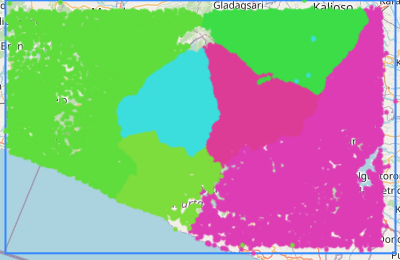
\includegraphics[width=\linewidth]{figures/partition_level_4.png}
        \caption{Partisi level 4 dengan ukuran $U_4=2^{17}$}
        \label{fig:c}
    \end{subfigure}
    \hfill
    \begin{subfigure}[b]{0.45\textwidth}
        \centering
        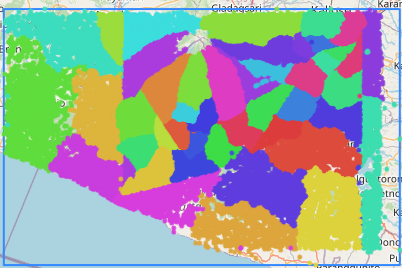
\includegraphics[width=\linewidth]{figures/partition_level_3.png}
        \caption{Partisi level 3 dengan ukuran $U_3=2^{14}$}
        \label{fig:d}
    \end{subfigure}

   
    \begin{subfigure}[b]{0.45\textwidth}
        \centering
        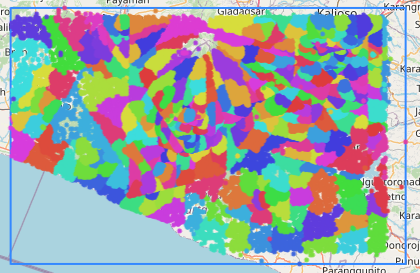
\includegraphics[width=\linewidth]{figures/partition_level_2.png}
        \caption{Partisi level 2 dengan ukuran $U_w=2^{11}$}
        \label{fig:c}
    \end{subfigure}
    \hfill
    \begin{subfigure}[b]{0.45\textwidth}
        \centering
        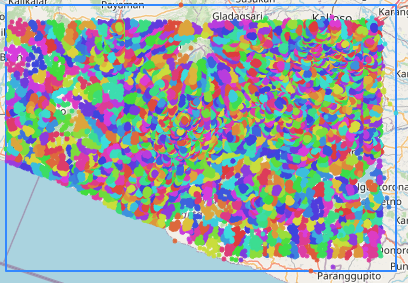
\includegraphics[width=\linewidth]{figures/partition_level_1.png}
        \caption{Partisi level 1 dengan ukuran $U_1=2^{8}$}
        \label{fig:d}
    \end{subfigure}

    \caption{Partisi \textit{multilevel} untuk graf jaringan jalan peta Openstreetmap wilayah Surakarta, Daerah Istimewa Yogyakarta, dan Klaten. Graf memiliki jumlah simpul sebanyak 481.978 dan jumlah sisi sebanyak 1.222.793.}
    \label{fig:mlp-inertial-flow}
\end{figure}

\begin{figure}[H]
    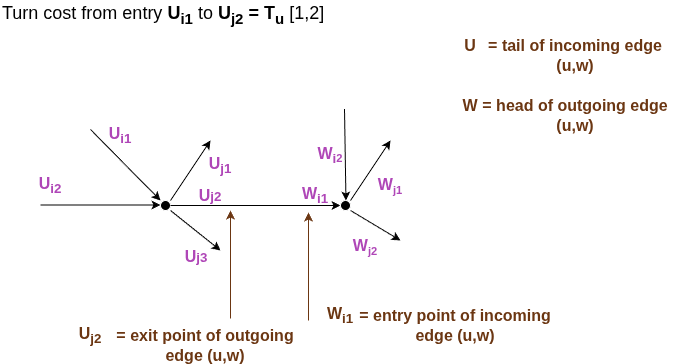
\includegraphics[scale=0.4]{figures/turn_cost_exit_entry.png}
    \caption{titik \textit{exit}, titik \textit{entry}, \textit{head point}, dan \textit{tail point} dari sisi $(u,w)$}
    \label{fig:crp-exit-entry-point}
\end{figure}


Untuk setiap sisi batas $(u,v)$, penulis menyimpan simpul \textit{overlay} $u'_{H}$ dan $v_{H}''$, dimana simpul $u'_{H}$  adalah simpul \textit{exit} dari sel $c_1(u)$ dan $v_{H}''$ adalah simpul \textit{entry} dari sel $c_1(v)$. Jika sisi $(v,u)$ juga terdapat dalam graf, maka kita juga menambahkan simpul $v'_H$ dan $u''_{H}$. Unutk meningkatkan lokalitas, kita mengurutkan ID dari simpul \textit{overlay} sedemikian hingga simpul batas dengan level tertinggi memiliki ID terendah, diikuti dengan simpul batas dengan level tetinggi kedua, dan seterusnya. Gambar~\ref{fig:crp-overlay2} menunjukkan ilustrasi dari sisi batas dan simpul \textit{overlay}/batas. Penulis membuat struktur data \textit{hash table} dengan \textit{key} berupa \textit{struct} berisi field simpul, \textit{turn order}, tipe simpul (\textit{exit} atau \textit{entry}) dengan value nya adalah ID dari simpul \textit{overlay}. Untuk menyimpan bobot dari sisi-sisi jalan pintas yang menghubungkan simpul-simpul \textit{overlay}/batas pada setiap sel di setiap level, penulis membuat struktur data \textit{array} satu dimensi bobot sisi jalan pintas W. Untuk setiap sel $C$  di dalam graf \textit{overlay} di setiap level, kita menyimpan $p_C$ (jumlah dari titik \textit{entry} dari sel), $q_C$ (jumlah dari titik \textit{exit} dari sel), dan $f_C$ (posisi di dalam \textit{array} $W$, dimana entri pertama dari matrix bobot dari sel $C$ disimpan), kita dapat mendapatkan bobot/biaya dari sisi jalan pintas antara titik \textit{entry} ke-$i$ dan titik \textit{exit} ke-$j$ dari sel $C$ dari $W[f_C+i\cdot q_C + j]$. Untuk dapat memetakan posisi simpul diantara simpul-simpul \textit{exit} atau \textit{entry} dari sel simpul ke ID dari simpul overlay nya, penulis membuat \textit{hash table} yang memetakan posisi \textit{entry}/\textit{exit} ke-$i$ dari sel $C$ pada level $l$ ke ID dari simpul \textit{overlay} yang bersesuaian. Untuk setiap simpul \textit{overlay} $v$, penulis juga menyimpan \textit{array} berukuran $L$ yag setiap indeksnya menyimpan posisi titik \textit{entry/exit} dari simpul pada sel dimana simpul berada.



\begin{figure}[H]
    \centering
    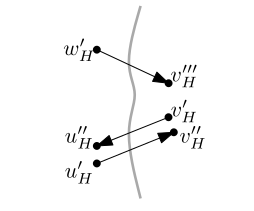
\includegraphics[]{figures/overlay_crp.png}
    \caption{graf \textit{overlay} yang terdiri dari sisi batas $(u,v)$, $(v,u)$, dan $(w,v)$ menghasilkan simpul \textit{overlay} $u'_{H},v_H'',v'_H,u''_H,w'_H, \text{ dan }v'''_H$ }
    \label{fig:crp-overlay2}
\end{figure}




\subsection{Fase Kustomisasi Tidak Bergantung Pada Waktu}
\label{subsec:tdcrp-kustomisasi}
Pada fase kustomisasi, penulis membuat sisi-sisi jalan pintas yang menghubungkan antara simpul \textit{entry} dan simpul \textit{exit} dari setiap sel dengan menggunakan bobot sisi yang terbaru. Penulis juga membangun \textit{array} bobot sisi-sisi jalan pintas W. Untuk membuat sisi-sisi jalan pintas, penulis menjalanakan algoritma Dijkstra secara \textit{bottom-up}. Untuk setiap sel $C$ dari graf \textit{overlay} level 1, penulis menjalankan algoritma \textit{turn-aware} Dijkstra pada setiap simpul \textit{entry} dari sel $C$ ke semua simpul \textit{exit} dari sel $C$. Untuk setiap sel $C$ dari graf level i (untuk i > 1), penulis menjalankan algoritma \textit{turn-aware} Dijkstra pada setiap simpul \textit{entry} ke semua simpul \textit{exit} dari sel $C$. Untuk level i > 1, algoritma Dijkstra dijalankan pada subgraf dari $H_{i-1}$ menggunakan sisi-sisi jalan pintas dari subsel-subsel dari sel $C$ yang mana cenderung lebih cepat jika dibandingkan dengan kustomisasi pada level 1. Untuk mengakselerasi fase kustomisasi, penulis menjalankan kustomisasi dari setiap sel secara \textit{multithreaded} dan menjalankan algoritma Dijkstra dari setiap simpul \textit{entry} secara \textit{multithreaded}. Gambar~\ref{fig:clique-crp} menunjukkan ilustrasi dari hasil kustomisasi. Pesudocode untuk algoritma kustomisasi pada level 1 ditunjukkan pada Algoritma~\ref{alg:crp-customization-level1} dan Algoritma~\ref{alg:crp-customization-levelhigher} untuk level $l>1$. Misalkan $K$ adalah jumlah partisi pada graf \textit{overlay} level 1 dan diasumsikan setiap partisi memiliki jumlah simpul yang sama ($|C_1|=|C_2|=\ldots =|C_K|$), maka kompleksitas dari algoritma kustomisasi adalaah $O(|E|+|V|\log \frac{|V|}{K})$.

\begin{figure}[H]
    \centering
    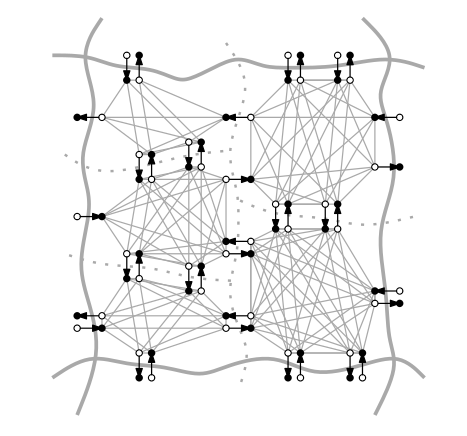
\includegraphics[]{figures/clique.png}
    \caption{graf overlay hasil kustomisasi}
    \label{fig:clique-crp}
\end{figure}




\begin{algorithm}
\caption{BUILDOVERLAYLEVELONE membuat \textit{clique} pada setiap sel-sel level 1 dan membuat \textit{array} bobot \textit{shortcut arcs} $W$}
\label{alg:crp-customization-level1}
\resizebox{\textwidth}{!}{%
\begin{minipage}{\textwidth}
\scriptsize
\begin{algorithmic}[1]
\setstretch{0.9}
\Procedure{BUILDOVERLAYLEVELONE}{$G, OG$}
    \For {$(cellId, cell) \in OG.CellsInLevel[1]$} \Comment{buat \textit{clique} dan \textit{array} bobot \textit{shortcut arcs} $W$  pada setiap sel level 1 }
        \For {$i = 0 \textbf{ to } cell.numEntryPoints$}
            \State $enVertex \gets OG.entryPoint[cell, i]$  \Comment{Dijkstra dari $entryVertex$ ke semua $exitVertex$ dari sel $cellId$}
            \State $enVertexEntryPos \gets G.entryPos[enVertex.originalEdge, enVertex]$
            \State $info \gets \emptyset$
            \State $oInfo \gets \emptyset$
            \State $Q \gets \emptyset: PriorityQueue$
            \State $info[enVertexEntryPos] \gets 0$
            \State $Q.insert(0, (enVertex, enVertexEntryPos))$
            \While{$Q \neq \emptyset$}
                \State $((u, uEntryPos), uTT) \gets Q.extractMin()$
                \For {$(v, oArc,exitPoint, turn) \in  G.E[u, uEntryPos]$}
                    \State $v \gets oArc.head$
                    \State $newTT \gets uTT + turn.cost + oArc.weight$
                    \State $vCellId \gets G.cellId[v]$
                    \If {$vCellId = cellId$}
                        \State $vEntryPos \gets oArc.entryPos$ \Comment{$v$ masih satu sel dengan $cellId$}
                        \State $((\cdot),vVisited) \gets info[vEntryPos]$
                        \If{$vVisited = false \textbf{ or } newTT < info[vEntryPos]$}
                            \State $info[vEntryPos] \gets newTT$
                            \State $Q.InsertOrDecreaseKey(newTT, (v, vEntryPos))$
                        \EndIf 
                    \Else 
                        \State $exitOverlay \gets G.overlayVertex[u, exitPoint, true]$ \Comment{$v$ tidak satu sel dengan $cellId$ }
                        \State $exitOverlayVisited \gets oInfo[exitOverlay]$  \Comment{$u$ adalah $exitVertex$ dari $cellId$}
                        \If {$exitOverlayVisited = false \textbf{ or } uTT + turn.cost < oInfo[exitOverlay]$}
                            \State $oInfo[exitOverlay] \gets uTT + turn.cost $
                        \EndIf 
                    \EndIf 
                \EndFor 
            \EndWhile 

            \For {$j =0  \textbf{ to }  cell.numExitPoints$}
                \State $exitVertex \gets OG.exitPoint[cell, j]$ \Comment{simpan bobot dari sisi \textit{shortcut} $(enVertex, exitVertex)$}
                \State $((\cdot), exitPointVisited) \gets oInfo[exitVertex]$
                \If{$exitPointVisited = false$}
                    \State $OG.W[cell.cellOffset + i \cdot cell.numberExitPoints + j]  \gets \infty$
                \Else 
                    \State $OG.W[cell.cellOffset + i \cdot cell.numberExitPoints + j]  \gets oInfo[exitPoint]$
                \EndIf 
            \EndFor 
        \EndFor
    \EndFor 
\EndProcedure
\end{algorithmic}
\end{minipage}%
}
\end{algorithm}

\begin{algorithm}
\caption{BUILDOVERLAY membuat \textit{clique} pada setiap sel-sel level $l>1$ dan membuat \textit{array} bobot \textit{shortcut arcs} $W$}
\label{alg:crp-customization-levelhigher}
\resizebox{\textwidth}{!}{%
\begin{minipage}{\textwidth}
\scriptsize
\begin{algorithmic}[1]
\setstretch{0.9}
\Procedure{BUILDOVERLAY}{$G, OG, l$}
    \For {$(cellId, cell) \in OG.CellsInLevel[l]$} \Comment{buat \textit{clique} dan \textit{array} bobot \textit{shortcut arcs} $W$  pada setiap sel level $l$ }
        \For {$i = 0 \textbf{ to } cell.numEntryPoints$}
            \State $enVertex \gets OG.entryPoint[cell, i]$  \Comment{Dijkstra dari $entryVertex$ ke semua $exitVertex$ dari sel $cellId$}
            \State $info \gets \emptyset$
            \State $oInfo \gets \emptyset$
            \State $Q \gets \emptyset: PriorityQueue$
            \State $info[enVertex] \gets 0$
            \State $Q.insert(0, (enVertex))$
            \While{$Q \neq \emptyset$}
                \State $((u), uTT) \gets Q.extractMin()$
                \For {$(exitVertex, wOffset) \in  OG.E[u, l-1]$} \Comment{\textit{traverse} semua sisi \textit{shortcut} $(enVertex,exitVertex)$ pada level $l-1$ }
                    \State $shortcutWeight \gets OG.W[wOffset]$
                    \State $newTT \gets uTT + shortcutWeight$
                    \State $(oldExitTT, exitVisited) \gets info[exitVertex]$
                    \If{$exitVisited = false \textbf{ or } newTT < oldExitTT$}
                        \State $info[exitVertex] \gets newTT$
                        \State $exitNeighborVertex \gets exitVertex.neighbor$ \Comment{\textit{traverse} neighbor dari $exitVertex$ yang berbeda sel dengan $sel$ dari $exitVertex$ pada level $l-1$}
                        \If {$TRUNCATEDTOEVEL(exitNeighborVertex.cellId, l) = cellId$}
                            \State $boundaryArcWeight \gets  exitVertex.edge.weight$ \Comment{$exitNeighborVertex$ masih satu sel dengan $exitVertex$ pada level $l$}
                            \State $newNeighborTT \ \gets newTT + boundaryArcWeight $
                            \State $(oldNTT, neighborVisited) \gets info[exitNeighborVertex]$
                            \If {$neighborVisited=false \textbf{ or } newNeighborTT < oldNTT$} 
                                \State $info[exitNeighborVertex] \gets newTT +boundaryArcWeight $
                                \State $Q.InsertOrDecreaseKey(info[exitNeighborVertex], exitNeighborVertex)$
                            \EndIf 
                        \EndIf 
                    \EndIf
                \EndFor 
            \EndWhile 

            \For {$j =0  \textbf{ to }  cell.numExitPoints$}
                \State $exitVertex \gets OG.exitPoint[cell, j]$ \Comment{simpan bobot dari sisi \textit{shortcut} $(enVertex, exitVertex)$}
                \State $((\cdot), exitPointVisited) \gets oInfo[exitVertex]$
                \If{$exitPointVisited = false$}
                    \State $OG.W[cell.cellOffset + i \cdot cell.numberExitPoints + j]  \gets \infty$
                \Else 
                    \State $OG.W[cell.cellOffset + i \cdot cell.numberExitPoints + j]  \gets oInfo[exitPoint]$
                \EndIf 
            \EndFor 
        \EndFor
    \EndFor 
\EndProcedure
\end{algorithmic}
\end{minipage}%
}
\end{algorithm}


\subsection{Fase Kueri Tidak Bergantung Pada Waktu}
\label{subsec:tdcrp-kueri}
Kueri pada Customizable Route Planning dilakukan dengan algoritma Turn Aware Multilevel Bidirectional Dijkstra (TA-MLBD). Kueri dari $s$ ke $t$ terdiri dari tiga bagian: prefiks maksimal di $c(s)$, suffiks maksimal $c(t)$, dan graf overlay $H$ yang berada diantara keduanya. Karena jarak antara simpul-simpul \textit{overlay}/batas pada graf overlay $H$ dan graf $G$ memiliki jarak yang sama, maka rute terpendeknya akan sama dengan rute terpendek pada graf $G$ \cite{Delling2015}. Input dari kueri adalah sisi asal $a_s$, sisi target $a_t$, graf $G$, dan graf \textit{overlay} $H =\cup_i H_i$. Tugas dari kueri adalah menghitung rute terpendek antara simpul \textit{head} $s$ dari $a_s$ dan simpul \textit{tail} dari $a_t$. Algoritma ini menggunakan empat \textit{priority queue}, yaitu \textit{forward overlay priority queue}(forwardOverlayPQ), \textit{backward overlay priority queue}(backwardOverlayPQ), \textit{forward original priority queue}(forwardPQ), dan \textit{backward original priority queue}(backwardPQ). \textit{Key} dari \textit{original priority queue}(PQ) TA-MLD adalah $(v,i,d)$, dimana $v$ adalah simpul $i$ adalah posisi titik \textit{entry} pada $v$, dan $d$ adalah label waktu tempuh. Algoritma menginisialisasi $(s,i,d)$ dengan $(s,i,0)$ dan $(t,i,d)$ dengan $(t,i,0)$. Dengan representasi seperti ini, ketika kita sedang melakukan relaksasi sisi $(u,v)\in A$, posisi titik \textit{entry} dari $u$ adalah $i$ dan posisi titik \textit{exit} dari sisi $(u,v)$ adalah $j$, kita dapat mendapatkan biaya \textit{turn}  dari sisi masuk ke-$i$ dan sisi keluar ke-$j$ dari simpul $u$  dari matriks \textit{turnTables}.

Diberikan simpul $v\in V$, \textit{query level} $l_{st}(v)$ adalah level tertinggi sedemikian hingga sel dari $v$ tidak sama dengan sel dari $s$ atau $t$. $l_{st}(v)$ adalah level $i$ tertinggi sedemikian hingga $c_i(v)\cap\{s,t\}=\emptyset$. $l_{st}(v)$ dihitung dengan $l_{st}(v)=\min\{MSD(PV(s), PV(v)), MSD(PV(t), PV(v))\}$, dimana $MSD(PV(s), PV(v))=\text{level tertingi dimana bit dari } PV(s) \text{ dan }PV(v) \text{ berbeda}$. \textit{Overlay priority queue} memilki key $(v, l_{st}(v)),\text{ dimana } v\in V$.

Pada setiap iterasi, algoritma mengambil nilai minimum dari kedua \textit{priority queue} utama, yaitu $\min_{pq}=\min\{\min_{forwardPQ}, \min_{backwardPQ}\}$ dan $\min_{overlayPQ}=\min\{\min_{forwardOverlayPQ}, \min_{backwardOverlayPQ}\}$. Jika $\min_{PQ} < \min_{overlayPQ}$, algoritma menjalankan subrutin Bidirectional Turn Aware Dijkstra (BTAD) dan jika $\min_{PQ} \geq \min_{overlayPQ}$, algoritma akan menjalankan subrutin Bidirectional Overlay Graph Dijkstra (BOGJ). Pada subrutin BTAD, subrutin mengambil nilai minimum dari $\min_{forwardPQ}$ dan $\min_{backwardPQ}$. Jika pada subrutin BTAD, nilai $\min_{forwardPQ}<\min_{backwardPQ}$, algoritma menjalankan subrutin Forward Turn Aware Dijkstra (FTAD) dan jika $\min_{forwardPQ}\geq\min_{backwardPQ}$, algoritma menjalankan Backward Turn Aware Dijkstra (BATAD). Untuk setiap simpul $u\in V$ yang sudah di $settle$ pada BTAD, subrutin mengiterasi semua sisi keluar $(u,v)\in A$ (jika menjalankan FTAD) atau sisi masuk $(v,u)\in A$ (jika menjalankan BATAD). Jika $l_{st}(v)=0$, subrutin akan menjalankan relaksasi sisi $(u,v)$ atau $(v,u)$ dengan menggunakan forwardPQ atau backwardPQ. Jika $l_{st}(v)\neq 0$, subrutin akan menjalankan relaksasi sisi  $(u,v)$ atau $(v,u)$ dengan menggunakan forwardOverlayPQ atau backwardOverlayPQ. Subrutin BOGJ diawali dengan mengambil nilai minimum dari kedua \textit{overlay priority queue}, yaitu $\min_{forwardOverlayPQ}$ dan $\min_{backwardOverlayPQ}$ . Jika  $\min_{forwardOverlayPQ} <\min_{backwardOverlayPQ}$, subrutin Forward Overlay Search akan dijalankan dan jika $\min_{forwardOverlayPQ} \geq \min_{backwardOverlayPQ}$, subrutin Backward Overlay Search akan dijalankan. Kedua subrutin tersebut menjalankan prosedur relaksasi sisi yang sama dengan Forward/Backward Turn Aware Dijkstra, namun pada kedua subrutin ini relaksasi sisi dilakukan pada sisi-sisi jalan pintas pada sel-sel graf \textit{overlay} level $l_{st}(u)$ dan \textit{turn cost} tidak dipertimbangkan dalam perhitungan waktu tempuh terpendek.

Penulis melakukan beberapa optimasi untuk mempercepat algoritma kueri. Pada saat relaksasi sisi jalan pintas $(u,v)$ atau $(v,u)$ pada subrutin Bidirectional Overlay Graph Dijkstra, subrutin menyimpan waktu tempuh terpendek dari simpul $v$ dan tidak langsung menambahkan/memperbarui simpul \textit{exit} $v$ ke $forwardOverlayPQ$ atau $backwardOverlayPQ$, subrutin langsung melakukan relaksasi sisi batas $(v,w)\in A$. Hal ini mengurangi jumlah operasi Priority Queue secara signifikan. Penulis juga melakukan optimisasi dengan cara mengalokasikan ukuran awal setiap struktur data yang dibutuhkan kueri dengan $\max\{len(c_1(s)),len(c_1(t))\}$, dimana $len(c_1(v))$ adalah jumlah simpul yang terletak pada sel yang mengandung simpul $v$. Implementasi Priority Queue dari algoritma kueri menggunakan varian Rank Pairing-Heap Priority Queue \cite{Haeupler2009} karena operasi \textit{decreaseKey} dari varian ini memiliki kompleksitas waktu terarmortisasi $O(1)$ dan operasi \textit{insert} memiliki kompleksitas waktu $O(1)$ akan membuat waktu eksekusi algoritma kueri semakin cepat. Algoritma~\ref{alg:crp-tamlbd} menunjukkan \textit{pseudocode} dari algoritma kueri Customizable Route Planning.


\begin{algorithm}
\caption{TAMLBD}
\label{alg:crp-tamlbd}
\resizebox{\textwidth}{!}{%
\begin{minipage}{\textwidth}
\scriptsize
\begin{algorithmic}[1]
\setstretch{0.9}
\Procedure{TAMLBD}{$as, at, G, OG$}
    \State $s \gets as.head$
    \State $t \gets at.tail$
    \State $sEntryPos \gets G.entryPos[as,s]$
    \State $tEntryPos \gets G.entryPos[at,t]$
    \State $fInfo, bInfo \gets \emptyset$
    \State $fQ,bQ \gets  \emptyset: PriorityQueue$
    \State $foQ,boQ \gets  \emptyset: PriorityQueue$
    \State $shortest \gets \infty$
    \State $fQ.insert(s, sEntryPos)$
    \State $bQ.insert(t, tEntryPos)$
    \While{$|fQ|+|foQ| > 0 \textbf{ dan } |bQ|+|boQ| > 0$ }
        \If {$\min\{\min_{fQ}, \min_{foQ} \} +\min\{\min_{bQ}, \min_{boQ} \} > shortest $}
            \State \textbf{break}
        \EndIf 
        \State $minQ=\min \{ \min_{fQ}, \min_{bQ}  \}$
        \State $minOQ=\min \{ \min_{foQ}, \min_{boQ}  \}$
        \If {$minQ < minOQ$}
            \State \Call{BDTurnAwareDijkstra}{$s,t,fInfo,bInfo,fQ, bQ, foQ, boQ, G, OG, shortest$}
        \Else 
             \State \Call{BDTurnAwareOverlayDijkstra}{$s,t,fInfo,bInfo,fQ, bQ, foQ, boQ, G, OG, shortest$}
        \EndIf
    \EndWhile   
    \State \textbf{return} $shortest, $ \Call{PATHUNPACKING}{$G,OG,fInfo,bInfo,PV(s),PV(t)$}
\EndProcedure
\end{algorithmic}
\end{minipage}%
}
\end{algorithm}


\begin{algorithm}
\caption{BidirectionalTurnAwareDijkstra}
\resizebox{\textwidth}{!}{%
\begin{minipage}{\textwidth}
\scriptsize
\begin{algorithmic}[1]
\setstretch{0.9}
\Procedure{BDTurnAwareDijkstra}{$s,t,fInfo,bInfo,fQ, bQ, foQ, boQ, G, OG, shortest$}
    \State $minRankF \gets fQ.findMin()$
    \State $minRankB \gets bQ.findMin()$
    \If {$minRankF <  minRankB$}
       \State  $((u, uEntryPos), \cdot) \gets fQ.deleteMin()$ \Comment{\textit{forward search} pada graf $G$}
        \For{$(oArc, turn, v) \in G.E[u,uEntryPos]$}
            \State $l_{st}(v) \gets \min\{MSD(PV(s), PV(v)), MSD(PV(t), PV(v))\}$
            \If{$l_{st}(v)=0$}
                \State $newTT \gets fInfo[uEntryPos].tt + oArc.weight + turn.cost$
                \State \Call{RELAX}{$v,u,uEntryPos, oArc, false, newTT,fInfo,bInfo, fQ,bQ, G, shortest$}
            \Else 
                \State \Call{RELAXOVERLAY}{$v,u,uEntryExitPos,oArc,false, shortest, G, newTT, l_{st}(v), fInfo, bInfo, foQ, boQ$}
            \EndIf 
        \EndFor 
    \Else 
        \State $((u, uExitPos), \cdot) \gets bQ.deleteMin()$ \Comment{\textit{backward search} pada graf $G$}
        \For{$(iArc, turn, v) \in  G.\overleftarrow{E}[u,uExitPos]$}
            \State $l_{st}(v) \gets \min\{MSD(PV(s), PV(v)), MSD(PV(t), PV(v))\}$
            \If{$l_{st}(v)=0$}
                \State $newTT\gets bInfo[uExitPos].tt + iArc.cost +turn.cost$
                \State \Call{RELAX}{$v,u,uExitPos,iArc,true,newTT,fInfo,bInfo,fQ,bQ, G, shortest$}
            \Else
                \State \Call{RELAXOVERLAY}{$v,u,uEntryExitPos,iArc, true, shortest, G, newTT, l_{st}(v), fInfo,bInfo, foQ,boQ$}
            \EndIf
        \EndFor 
        
    \EndIf 
\EndProcedure
\end{algorithmic}
\end{minipage}%
}
\end{algorithm}


\begin{algorithm}
\caption{RELAX}
\resizebox{\textwidth}{!}{%
\begin{minipage}{\textwidth}
\scriptsize
\begin{algorithmic}[1]
\setstretch{0.9}
\Procedure{RELAX}{$v,u,uEntryPos, Arc, backward, newTT, fInfo,bInfo, fQ,bQ, G, shortest$}
    \If {$backward = false$}
        \State $vEntryPos \gets G.entryPos[arc,v] $
        \State $((\cdot), vVisited) \gets fInfo[vEntryPos]$
        \If {$newTT < fInfo[vEntryPos].tt \textbf{ or } vVisited = false$}
            \State $fInfo[vEntryPos] \gets (newTT, u , uEntryExitPos)$ \Comment{relaksasi sisi keluar $(u,v)\in G.E$}
            \State $fQ.InsertOrDecreaseKey(newTT, (v, vEntryPos))$ 
            \For{$(voArc, vExitPos, turn, \cdot) \in G.E[v, arc.entryPos]$} 
                \State $((\cdot), visitedByBackward) \gets bInfo[vExitPos]$ \Comment{cek apakah $v$ sudah dikunjungi pada kedua \textit{search}}
                \If{$visitedByBackward = true$}
                    \State $newTT \gets fInfo[vEntryPos].tt + turn.cost + binfo[vExitPos].tt$
                    \If{$newTT < shortest$}
                        \State $shortest=  newTT$
                    \EndIf
                \EndIf 
            \EndFor 
        \EndIf 
    \Else 
        \State $vExitPos \gets G.exitPos[arc, v]$
        \State $((\cdot),  vVisited) \gets bInfo[vExitPos]$
        \If{$newTT < bInfo[vExitPos].tt \textbf{ or } vVisited = false$}
            \State $bInfo[vExitPos] \gets (newTT, u, uExitPos)$ \Comment{relaksasi sisi masuk $(u,v)\in G.\overleftarrow{E}$}
            \State $bQ.InsertOrDecreaseKey(newTT, (v, vExitPos))$
            \For{$(viArc, vEntryPos, turn, \cdot) \in G.\overleftarrow{E}[v,arc.exitPos]$}
                \State $((\cdot), visitedByForward) \gets fInfo[vEntryPos]$  \Comment{cek apakah $v$ sudah dikunjungi pada kedua \textit{search}}
                \If {$visitedByForward=true$}
                    \State $newTT \gets fInfo[vEntrypos].tt + turn.cost + bInfo[vExitPos].tt$
                    \If {$newTT < shortest$}
                        \State $shortest \gets newTT$
                    \EndIf 
                \EndIf 
            \EndFor 
        \EndIf 
        \State 
    \EndIf
\EndProcedure
\end{algorithmic}
\end{minipage}%
}
\end{algorithm}

\begin{algorithm}
\caption{RELAXOVERLAY relaksasi sisi keluar $(u,v)$. Simpul $v$ tidak satu sel dengan simpul $s$ dan $t$ pada level $l_{st}(v)$}

\resizebox{\textwidth}{!}{%
\begin{minipage}{\textwidth}
\scriptsize
\begin{algorithmic}[1]
\setstretch{0.9}
\Procedure{RELAXOVERLAY}{$v,u,uEntryExitPos,arc,backward,shortest,G, newTT, l_{st}(v), fInfo,bInfo, foQ,boQ$}
    \If {$backward = false$}
        \State $vOverlay \gets G.overlayVertex[v, arc.entryPos, backward]$
        \State $((\cdot), vOverlayVisited) \gets fInfo[vOverlay]$
        \If {$vOverlayVisited = false \textbf{ or } newTT < fInfo[vOverlay].tt$}
            \State $fInfo[vOverlay] \gets (newTT, u, uEntryExitPos)$ \Comment{relaksasi sisi keluar $(u,v)\in G.E$}
            \State $foQ.InsertOrDecreaseKey(newTT, (v, l_{st}(v)))$
            \State $((\cdot), visitedByBackward) \gets bInfo[vOverlay]$ \Comment{cek apakah $v$ sudah dikunjungi pada kedua \textit{search}}
            \If {$visitedByBackward = true \textbf{ and } fInfo[vOverlay].tt + bInfo[vOverlay].tt  < shortest$} 
                \State $shortest \gets fInfo[vOverlay].tt + bInfo[vOverlay].tt$ 
            \EndIf
        \EndIf
    \Else 
        \State $vOverlay \gets G.overlayVertex[v, arc.exitPos, backward]$
        \State $((\cdot), vOverlayVisited) \gets bInfo[vOverlay]$
        \If {$vOverlayVisited = false \textbf{ or } newTT < bInfo[vOverlay].tt$}
            \State $bInfo[vOverlay] \gets (newTT, u, uEntryExitPos)$ \Comment{relaksasi sisi masuk $(u,v)\in G.\overleftarrow{E}$}
            \State $boQ.InsertOrDecreaseKey(newTT, (v, l_{st}(v)))$
            \State $((\cdot), visitedByForward) \gets fInfo[vOverlay]$  \Comment{cek apakah $v$ sudah dikunjungi pada kedua \textit{search}}
            \If {$visitedByForward = true \textbf{ and } fInfo[vOverlay].tt + bInfo[vOverlay].tt < shortest$}
                \State $shortest \gets fInfo[vOverlay].tt + bInfo[vOverlay].tt$
            \EndIf
        \EndIf
    \EndIf 
    
\EndProcedure
\end{algorithmic}
\end{minipage}%
}
\end{algorithm}



\begin{algorithm}
\caption{BidirectionalOverlayGraphDijkstra}
\resizebox{\textwidth}{!}{%
\begin{minipage}{\textwidth}
\scriptsize
\begin{algorithmic}[1]
\setstretch{0.8}
\Procedure{BidirectionalOverlayGraphDijkstra}{$s,t,fInfo,bInfo,fQ, bQ, foQ, boQ, G, OG, shortest$}
    \State $minRankOF \gets foQ.findMin()$
    \State $minRankOB \gets boQ.findMin()$
    \If {$minRankOF < minRankOB $}
        \State $((u, l_{st}(u)), \cdot) \gets foQ.deleteMin()$ \Comment{\textit{forward search} pada graf \textit{overlay} OG}
        \For {$(wOffset, v) \in OG.E[u, l_{st}(u)]$} \Comment{\textit{traverse} semua sisi \textit{shortcut} $(u,v)\in OG.E$ pada level $l_{st}(u)$}
            \State $newTT \gets fInfo[u].tt + OG.W[wOffset] $
            \State $((\cdot), vVisited) \gets fInfo[v]$
            \If {$vVisited = false \textbf{ or } newTT < fInfo[v].tt$}
                \State $fInfo[v] \gets (newTT, u.originalId, u)$
                \State $((\cdot), visitedByBackward) \gets bInfo[v]$
                \If {$visitedByBackward=true \textbf{ and } fInfo[v].tt + bInfo[v].tt < shortest$}
                    \State $shortest \gets fInfo[v].tt + bInfo[v].tt$
                \EndIf 
                \State $w \gets OG.neighborOverlayVertex[v]$  \Comment{\textit{traverse} simpul tetangga $w$ dari $v$ yang berbeda sel dengan $v$ pada level $l_{st}(u)$}
                \State $l_{st}(w) \gets \min \{ MSD(PV(s), PV(w)), MSD(PV(t), PV(w)) \}$
                \State $vOutArc \gets v.outArc$
                \If {$l_{st}(w)= 0$}
                    \State \Call{RELAX}{$w.originalId,v,v.originalId, vOutArc, false, newTT,fInfo,bInfo, fQ,bQ, G, shortest$}
                \Else 
                    \State \parbox[t]{\dimexpr\linewidth-\algorithmicindent}{%
                  \Call{RELAXOVERLAY}{$w.originalId,v,v.originalId,vOutArc,false, shortest, G, newTT,$\\
                  \hspace{2em}$l_{st}(w), fInfo, bInfo,foQ, boQ$}                }
                \EndIf
            \EndIf
        \EndFor 
    \Else 
        \State $((u, l_{st}(u)), \cdot) \gets boQ.deleteMin()$  \Comment{\textit{backward search} pada graf \textit{overlay} OG}
        \For {$(wOffset, v) \in OG.\overleftarrow{E}[u, l_{st}(u)]$} \Comment{\textit{traverse} semua sisi \textit{shortcut} $(u,v)\in OG.\overleftarrow{E}$ pada level $l_{st}(u)$}
            \State $newTT \gets fInfo[u].tt + OG.W[wOffset] $
            \State $((\cdot), vVisited) \gets bInfo[v]$
            \If {$vVisited = false \textbf{ or } newTT < bInfo[v].tt$}
                \State $bInfo[v] \gets (newTT, u.originalId, u)$
                \State $((\cdot), visitedByForwad) \gets fInfo[v]$
                \If {$visitedByForwad=true \textbf{ and } fInfo[v].tt + bInfo[v].tt < shortest$}
                    \State $shortest \gets fInfo[v].tt + bInfo[v].tt$
                \EndIf 
                \State $w \gets OG.neighborOverlayVertex[v]$ \Comment{\textit{traverse} simpul tetangga $w$ dari $v$ yang berbeda sel dengan $v$ pada level $l_{st}(u)$}
                \State $l_{st}(w) \gets \min \{ MSD(PV(s), PV(w)), MSD(PV(t), PV(w)) \}$
                \State $vInArc \gets v.inArc$
                \If {$l_{st}(w)= 0$}
                    \State \Call{RELAX}{$w.originalId,v,v.originalId, vInArc, true, newTT,fInfo,bInfo, fQ,bQ, G, shortest$}
                \Else 
                    \State \parbox[t]{\dimexpr\linewidth-\algorithmicindent}{%
                  \Call{RELAXOVERLAY}{$w.originalId,v,v.originalId,vInArc,true, shortest, G, newTT,$\\
                  \hspace{2em}$l_{st}(w), fInfo, bInfo,foQ, boQ$}                }
                \EndIf
            \EndIf
        \EndFor
    \EndIf 
\EndProcedure
\end{algorithmic}
\end{minipage}%
}
\end{algorithm}

\begin{algorithm}
\caption{Time-Dependent Dijkstra menghitung label final $\tau[u]=EA_G(s,u,\tau_0)$ untuk semua simpul $u$ yang dapat dijangkau (dan $\tau[u]=\in $ jika $u$ tidak dapat dijangkau.} 
\label{alg:td-dijkstra}
\resizebox{\textwidth}{!}{%
\begin{minipage}{\textwidth}
\scriptsize
\begin{algorithmic}[1]
\setstretch{0.9}
\Procedure{tdDijkstra}{$s: V, \tau_0: \mathbb{R}$}
    \State $\tau[u]=\infty\text{ untuk semua } u\in V, \tau[s]=\tau_0$ \Comment{nilai awal label simpul}
    \State $p[u]=\bot \text{ untuk semua }u\in V$  \Comment{nilai awal informasi \textit{predecessor}}
    \Procedure{tdRelax}{$u\rightarrow_fv: Edge, \tau, p, Q: PriorityQueueReference$}
        \If{$arr f(\tau[u])\geq\tau[v]$}
            \State \textbf{return}
        \EndIf
        \State $\tau[v]=\min\{\tau[v],arr f(\tau[u])\}$  \Comment{perbarui label simpul $v$}
        \State $p[v]=u$     \Comment{perbarui informasi \textit{predecessor} dari $v$}
        \If{$v\notin Q$}
            \State $Q.insert(v,\tau[v])$
        \Else
           \State $Q.decreaseKey(v,\tau[v])$
        \EndIf
    \EndProcedure
    \State $Q=\{s,\tau[s]\}: PriorityQueue$
    \While{$Q \neq \emptyset$}
        \State $u=Q.deleteMin()$
        \For{$u\rightarrow_fv\in E$}
            \State \Call{tdRelax}{$u\rightarrow_fv,\tau,p,Q$}
        \EndFor
    \EndWhile
\EndProcedure
\end{algorithmic}
\end{minipage}%
}
\end{algorithm}

\begin{algorithm}
\caption{ProfileSearch menghitung label final $f[u]=TTP_G(s,u)$ untuk semua simpul $u$.} 
\label{alg:profileSearch}
\resizebox{\textwidth}{!}{%
\begin{minipage}{\textwidth}
\scriptsize
\begin{algorithmic}[1]
\setstretch{0.9}
\Procedure{ProfileSearch}{$s: V, \tau_0: \mathbb{R}$}
    \State $\tau[u]=\infty\text{ untuk semua } u\in V, \tau[s]=\tau_0$ \Comment{nilai awal label simpul}
    \State $p[u]=\emptyset \text{ untuk semua }u\in V$  \Comment{nilai awal informasi \textit{predecessor}}
    \Procedure{profileRelax}{$u,v:V,g_{new}: TTF, f,p, Q: PriorityQueueReference$}
        \If {$g_{new}\geq f[v](\tau) \text{ untuk semua } \tau \in \mathbb{R}$}
            \State \textbf{return} 
        \EndIf
        \If{$g_{new}(\tau)<f[v](\tau) \text{ untuk semua } \tau\in \mathbb{R}$}
            \State $p[v]=\emptyset$ \Comment{hapus \textit{predecessor} kurang optimal}
        \EndIf
        \State $f[v]=min(f[v],g_{new})$ \Comment{perbarui label tentatif dari simpul $v$}
        \State $p[v]=\{u\}\cup p[v]$ \Comment{perbarui \textit{predecessor} tentatif dari simpul $v$}
        \If{$v\notin Q$}
            \State $Q.insert(v, \min f[v])$
        \Else 
            \State $Q.decreaseKey(v, \min f[v])$
        \EndIf
    \EndProcedure
    \State $Q=\{ (s,0)\}: PriorityQueue$
    \While{$Q\neq \emptyset$}
        \State $u=Q.deleteMin()$
        \For {$u\rightarrow v \in V \text{ dengan TTF } f_{uv} $}
            \Call{profileRelax}{$u,v,f_{uv}\ \circ \ f[u], f, p, Q$}
        \EndFor
    \EndWhile
    
\EndProcedure
\end{algorithmic}
\end{minipage}%
}
\end{algorithm}

Algoritma kueri paling banyak akan mengunjungi semua simpul dari sel $s$ pada level 1, semua simpul dari sel $t$ pada level 1, dan semua simpul batas dari semua sel dari setiap level graf \textit{overlay}. Misalkan $U_1$, $E_1$, dan $B$ secara berturut-turut adalah jumlah maksimum simpul dari setiap sel pada graf \textit{overlay} level 1, jumlah maksimum sisi dari setiap sel pada graf \textit{overlay} level 1, dan jumlah simpul batas  dari semua sel dari setiap level graf \textit{overlay}. Kasus terburuk dari algoritma kueri adalah ketika semua sisi batas memiliki dua arah, sehingga jumlah maksimum sisi jalan pintas dari setiap sel dari setiap level graf \textit{overlay} adalah $B^2$. Karena algoritma kueri menggunakan implementasi \textit{Rank Pairing-Heap} sebagai Priority Queue, maka kompleksitas waktu algoritma kueri adalah $O(E_1+U_1\log U_1+B^{2}+B \log B)$.




\subsection{Fase Kustomisasi Bergantung Pada Waktu}
\label{subsec:tdcrp-timedependent-customization}
Untuk mengadaptasi Customizable Route Planning pada graf yang bergantung pada waktu, penulis menggunakan metode Time-Dependent Customizable Route Planning yang diperkenalkan pada penelitian oleh \cite{Baum2016}. Kustomisasi untuk Time-Dependent Customizable Route Planning dilakukan dengan menjalankan algoritma ProfilSearch~\ref{alg:profileSearch} dari setiap simpul batas \textit{entry} $u\in C$ pada semua sel $C\in\mathcal{C}^{i}, i\geq 1$ ke setiap simpul batas \textit{exit} $v\in C$ lain untuk mendapatkan \textit{time-dependent shortcuts}.  Tetapi, pada level i > 1, algoritma ProfileSearch dijalankan pada subgraf dari $H_{i-1}$ menggunakan sisi-sisi jalan pintas dari subsel-subsel dari sel $C\in\mathcal{C}^i, i>1$. Optimasi dapat dilakukan dengan memanfaatkan $f^{\max}\text{ dan }f^{\min} \text{ dari setiap \textit{travel-time-profile} } f $. Sebelum merelaksasi sisi $(u,v)$, cek apakah $f_{u}^{\min}+f_{(u,v)}^{\min}\leq f^{max}$, yaitu nilai minimum dari hasil operasi $link(f_u,f_{uv})$ kurang dari sama dengan nilai maksimum label pada simpul $v$. Jika kondisi ini terpenuhi, lakukan relaksasi sisi $(u,v)$. Setelah menjalankan operasi $link(f_u,f_{uv})$, kita mendapatkan nilai label tentatif $\tilde{f}_v$,$\tilde{f}_v^{max}$, dan $\tilde{f}_v^{min}$. Jika kondisi $\tilde{f}_v^{min}>f_v^{max}$, operasi $merge(f_u,f_{uv}\ \circ \ f[u])$ tidak perlu dijalankan. Jika kondisi $\tilde{f}_v^{max}<f_v^{min}$, ganti $f_v$ dengan $\tilde{f}_v$. Jika kedua kondisi tersebut tidak dipenuhi, jalankan operasi $merge(f_u,f_{uv}\ \circ \ f[u])$. Penulis menjalanakan fase kustomisasi dengan memanfaatkan $multithreading$, dimana setiap sel diproses di \textit{thread} yang berbeda.


\subsection{Integrasi Dengan Data Lalu Lintas Terbaru dan Prediksi Kecepatan Lalu Lintas}
\label{subsec:tdcrp-traffic-update}
Kustomisasi saat terjadi pembaruan data lalu lintas hanya dilakukan pada sel-sel $C$ yang terdampak pada pembaruan. Misalkan $e_1=(u_1,v_1),\ldots,e_k=(u_k,v_k)$ adalah sisi-sisi di dalam suatu sel $C_i^l \text{ pada level }l$ yang bobotnya diperbarui akibat data pembaruanlalu lintas atau prediksi lalu lintas. Semua pembaruan data lalu lintas diberikan sebagai fungsi parsial $f:[\pi',\pi'']\rightarrow \mathbb{R}^+$, dimana $\pi'\in \Pi \text{ dan }\pi''\in \Pi$ secara berturut-turut adalah awal dan akhir dari rentang waktu dari pembaruan data lalu lintas. Misalkan $f_1,\ldots,f_k$ adalah fungsi parsial dari setiap sisi yang diperbarui dan $\tau$ adalah waktu saat pembaruan data lalu lintas dilakukan.  Untuk memperbarui sisi-sisi jalan pintas dalam sel-sel dari $C_i^l$, jalankan kueri LD dari simpul-simpul $head$ dari semua sisi yang diperbarui. Kustomisasi diawali dengan memasukkan $u_1,\ldots,u_k$ ke dalam Priority Queue dan menetapkan label waktu tempuh dari $u_i,i\in\{1,\ldots,k\}$ dengan $\pi''$. Sisi-sisi batas yang terjangkau oleh kueri LD ditandai sebagai terdampak oleh pembaruan data lalu lintas. Pencarian dihentikan ketika label waktu tempuh dari simpul yang baru saja \textit{settled} dibawah $\tau$. Kustomisasi dilanjutkan dengan menjalankan alogoritma ProfileSearch~\ref{alg:profileSearch} pada simpul-simpul yang ditandai pada sel $C_i^l$.

\subsection{Fase Kueri Bergantung Pada Waktu}
\label{subsec:tdcrp-time-dependent-query}
Algoritma kueri pada Time-Dependent Customizable Route Planning hampir sama dengan algoritma kueri Time-Independent Customizable Route Planning. Perbedaannya, kueri dijalankan satu arah saja dan menggunakan Time-Dependent Dijkstra yang dimodifikasi. Modifikasi algoritma Time-Dependent Dijsktra diperlukan agar pencarian dapat memanfaatkan sisi-sisi jalan pintas pada graf \textit{overlay}, sehingga ruang pencarian dipangkas. Kompleksitas waktu dari algoritma kueri adalah $O(E_1+U_1\log U_1+B^{2}+B \log B)$. Hal ini disebabkan karena algoritma kueri paling banyak akan mengunjungi semua simpul dari sel $s$ pada level 1, semua simpul dari sel $t$ pada level 1, dan semua simpul batas dari semua sel dari setiap level graf overlay. 



\begin{algorithm}
\caption{Time-Dependent Dijkstra CRP menghitung label final $\tau[u]=EA_G(s,u,\tau_0)$ untuk semua simpul $u$ yang dapat dijangkau (dan $\tau[u]=\in $ jika $u$ tidak dapat dijangkau.} 
\label{alg:td-dijkstra-crp}
\resizebox{\textwidth}{!}{%
\begin{minipage}{\textwidth}
\scriptsize
\begin{algorithmic}[1]
\setstretch{0.9}
\Procedure{tdDijkstraCRP}{$s,t: V, \tau_0: \mathbb{R}$}: $(\mathbb{R}, Set, Set, Set)$
    \State $\tau[u]=\infty\text{ untuk semua } u\in V, \tau[s]=\tau_0$ \Comment{nilai awal label simpul}
    \State $p[u]=\bot \text{ untuk semua }u\in V$  \Comment{nilai awal informasi \textit{predecessor}}
    

    \State $Q=\{s,sEntryPos,\tau[s]\}: PriorityQueue$
    \State $shortestTimeTravel=\infty$
    \State $overlayQ =\emptyset: PriorityQueue $
    \While{$Q \neq \emptyset \textbf{ or } overlayQ\neq \emptyset $}
        
        \If{$overlayQ =\emptyset \textbf{ or } Q.getMin() < overlayQ.getMin()$}
            \State $(u,uEntryPos)=Q.deleteMin()$
            \If {$u\in Q \textbf{ and } dist[u]>shortestTimeTravel$}
                \State \textbf{break}
            \EndIf
            \If{$u=t$}
                \State $shortestTimeTravel=\min\{shortestTimeTravel,dist[u]\}$
            \EndIf
            \For{$(u\rightarrow_fv,turnCost_{uv})\in E$}               
                \State \Call{tdRelaxCRP}{$u\rightarrow_fv,v,u, uEntryPos,\tau,p,Q,overlayQ,turnCost_{uv}$}
            \EndFor
        \Else 
            \State $u=overlayQ.deleteMin()$
            \If {$u\in Q \textbf{ and } dist[u]>shortestTimeTravel$}
                \State \textbf{break}
            \EndIf
            \State $l_{st}(u)=\min\{MSD(PV(s), PV(u)), MSD(PV(t), PV(u))\}$
            \For{$(u\rightarrow_{f_{shortcut\_uv}}v) \in E_{\mathcal{C}^{l_{st}(u)}}$}
                \State \Call{tdRelaxOverlayCRP}{$u\rightarrow_{f_{shortcut\_uv}}v,u, \tau, p, Q,overlayQ$}
            \EndFor
        \EndIf
    \EndWhile
    \State \textbf{return} $shortestTimeTravel, $ \Call{pathUnpacking}{p}, $p, \tau$
\EndProcedure
\end{algorithmic}
\end{minipage}%
}
\end{algorithm}


\begin{algorithm}
\caption{Relaksasi sisi pada kueri TD-Dijkstra untuk Time-DependentDikstra} 
\label{alg:td-dijkstra-crp}
\resizebox{\textwidth}{!}{%
\begin{minipage}{\textwidth}
\scriptsize
\begin{algorithmic}[1]
\setstretch{0.9}
    \Procedure{tdRelaxCRP}{$u\rightarrow_fv: Edge,v,u,uEntryPos, \tau, p, Q,overlayQ,turnCost_{uv}$}
        \If{$arr f(\tau[u])\geq\tau[v] $}
            \State \textbf{return}
        \EndIf
    
        \State $l_{st}(v)=\min\{MSD(PV(s), PV(v)), MSD(PV(t), PV(v))\}$
        \If{$l_{st}(v)=0$}
            \If{$v\notin Q \textbf{ or } (arr f(\tau[u])+turnCost_{uv})<\tau[v]$}
                \State $\tau[v]=\min\{\tau[v],(arr f(\tau[u])+turnCost_{uv})\}$  \Comment{perbarui label simpul $v$. $O(\mid f_u\mid +\mid f_{uv}\mid )$}
                \State $p[v]=u$     \Comment{perbarui informasi \textit{predecessor} dari $v$}
                \If{$v\notin Q$}
                    \State $Q.insert(v,GetEntryPos(v),\tau[v])$
                \Else
                   \State $Q.decreaseKey(v,GetEntryPos(v),\tau[v])$
                \EndIf
            \EndIf
        \Else
            \State $vOverlay=GetOverlayVertex(v,uEntryPoint)$
            \If{$vOverlay \notin overlayQ \textbf{ or } (arr f(\tau[u])+turnCost_{uv})<\tau[vOverlay]$}
                \State $\tau[vOverlay]=\min\{\tau[vOverlay],(arr f(\tau[u])+turnCost_{uv})\}$  \Comment{perbarui label simpul $vOverlay$}
                \State $p[vOverlay]=u$     \Comment{perbarui informasi \textit{predecessor} dari $vOverlay$}
                \If{$vOverlay \notin overlayQ$}
                    \State $overlayQ.insert(vOverlay,\tau[vOverlay])$
                \Else
                   \State $overlayQ.decreaseKey(vOverlay,\tau[vOverlay])$
                \EndIf
            \EndIf
        \EndIf
    \EndProcedure


    \Procedure{tdRelaxOverlayCRP}{$u\rightarrow_{f_{shortcut\_uv}}v,u, \tau, p, Q,overlayQ$}
        \If{$arr f_{shortcut\_uv}(\tau[u])\geq\tau[v] $}
            \State \textbf{return}
        \EndIf
        
       
        \If{$v\notin Q \textbf{ or } arr f_{shortcut\_uv}(\tau[u])< \tau[v]$}
            \State $\tau[v]=\min\{\tau[v],arr f_{shortcut\_uv}(\tau[u])\}$  \Comment{perbarui label simpul $v$. $O(\mid f_u\mid +\mid f_{uv}\mid )$}
            \State $p[v]=u$     \Comment{perbarui informasi \textit{predecessor} dari $v$}
            \State $w=v.neighborOverlayVertex$
            \State $vOverlay=GetOverlayVertex(v)$
            \State $(vOutEdge,f_{vw})=vOverlay.GetOutEdge()$
            \State $l_{st}(w)=\min\{MSD(PV(s), PV(w)), MSD(PV(t), PV(w))\}$
            \If{$l_{st}(w)=0$} \Comment{sel dari $w$ pada level-1 sama dengan sel $s$ atau $t$ pada level 1}
                \If{$w\notin Q \textbf{ or } arr f_{vw}(\tau[v])<\tau[w]$}
                    \State $\tau[w]=\min\{\tau[w],(arr f_{vw}(\tau[v])\}$  
                    \State $p[w]=v$     
                    \If{$w\notin Q$}
                        \State $Q.insert(w,GetEntryPos(w),\tau[w])$
                    \Else
                     \State   $Q.decreaseKey(w,GetEntryPos(w),\tau[w])$
                    \EndIf
                \EndIf
            \Else
                \If{$w\notin overlayQ \textbf{ or } arr f_{vw}(\tau[v])<\tau[w]$}
                    \State $\tau[w]=\min\{\tau[w],arr f_{vw}(\tau[v])\}$  
                    \State $p[w]=v$    
                    \If{$w\notin overlayQ$}
                        \State $overlayQ.insert(w,\tau[w])$
                    \Else
                      \State  $overlayQ.decreaseKey(w,\tau[w])$
                    \EndIf
                \EndIf          
            \EndIf
                
            
        \EndIf
       
    \EndProcedure
\end{algorithmic}
\end{minipage}%
}
\end{algorithm}


\subsection{Path Unpacking}
\label{subsec:tdcrp-path-unpacking}
Rute terpendek yang didapat dari algoritma CRP mungkin memiliki banyak sisi jalan pintas. Padahal dalam aplikasi navigasi, rute yang ditampilkan di peta adalah sisi-sisi orisinal dari graf yang merupakan segmen jalan pada \textit{road networks} dan bukan sisi-sisi jalan pintas. \textit{Path unpacking} adalah algoritma untuk mendapatkan sisi-sisi orisinal dari rute terpendek CRP yang mengandung sisi jalan pintas. \textit{Path unpacking} melakukan \textit{unpacking} sisi jalan pintas level-$i$ $(v,w)$ dengan menjalankan algoritma dijkstra dua arah antara $v$ dan $w$ secara rekursif pada subsel-subsel dari sel level $i$ yang mengandung sisi jalan pintas. Untuk mempercepat \textit{path unpacking}, penulis membuat \textit{cache} dengan kebijakan pembaruan $LRU$ untuk menyimpan \textit{unpacked path} dari sisi jalan pintas $(v,w,i)$ pada \textit{overlay} level-$i$ beserta dengan sisi-sisi pada level $i-1$ yang mewakili sisi jalan pintas tersebut.




	\section{Online Map-Matching Menggunakan Multiple Hypothesis Technique}
	\label{multiple hypothesis technique}
		\subsection{Formulasi Masalah}
\label{subsec:omm-preliminaries}
Sekuens data dari sejumlah K data titik GPS yang dikumpulkan oleh kendaraan didefinisikan dengan \textit{trajectory} $g_{1:K}$. Setiap data titik GPS memiliki data $(g_k.t,g_k.lat,g_k.lng,g_k.v)$ yang secara berturut-turut adalah waktu pengambilan titik GPS, \textit{latitude}, \textit{longitude}, dan kecepatan. Kecepatan dapat diambil dari diferensial antara dua titik GPS. Jaringan jalan adalah sebuah graf berarah $G(V,E)$ dimana $V$ adalah himpunan dari simpul-simpul dan $E$ adalah himpunan dari sisi-sisi yang merepresentasikan segmen jalan. Setiap segmen jalan $e\in E$ memiliki 4 data $(e.id, e.l, e.start, e.end)$ yang secara berturut-turut adalah ID, panjang, titik awal, dan titik akhir dari sisi $e$. Diberikan sebuah rute $r_{1:k}$ adalah sekuens dari sejumlah K segmen-segmen jalan yang sesuai dengan lintasan yang diberikan \textit{trajectory} $g_{1:k}$. Setiap segmen jalan $r_k\in E$ merepresentasikan segmen jalan dimana kendaraan sedang berada pada \textit{time step} $k$. \textit{Online map matching} bertugas untuk menentukan segmen jalan $r_k$ pada setiap \textit{time step} $1\leq k \leq K$ dengan hanya menggunakan titik-titik GPS terdahulu $\{g_i\mid 1\leq i\leq k\}$. Rute $\tau$ adalah rute yang dimulai dari segmen jalan $r_k$ yang mempunyai panjang tak hingga. $\tau$ adalah sekuens dari segmen-segmen jalan yang saling terhubung $\tau=\{e_1\rightarrow e_2\ldots\}, 1 \leq i \leq \infty, \text{ dimana } e_1=r_k, e_i.end=e_{i+1}.start$. Probabilitas rute $\tau$ didefinisikan dengan:
\begin{equation}
    p(\tau)=\prod_{i=1}^{\infty}p(e_i\rightarrow e_{i+1})
\end{equation}

\textit{Online map-matching} dapat dilakukan dengan menggunakan \textit{Bayesian filtering} (\cite{Taguchi2019}). \textit{Bayesian filtering} memberikan estimasi probabilitas posterior $p(r_k\mid g_{1:k})$ untuk setiap langkah pengambilan sampel $k$. Probabilitas posterior dapat dihitung melalui teorema bayes sebagai berikut:
\begin{equation}
    p(r_k\mid g_{1:k})=\frac{p(g_k\mid r_k,g_{1:k-1})p(r_k,g_{1:k-1})}{p(g_k\mid g_{1:k-1})}
\end{equation}
Dengan mengasumsikan independensi bersyarat,$g_k \perp\!\!\!\perp g_{1:k-1} \mid r_k $ posterior dapat dihitung dengan:

\begin{align}
p(r_k \mid g_{1:k}) 
&\propto p(g_k \mid r_k)\, p(r_k \mid g_{1:k-1}) \notag\\
&\propto p(g_k \mid r_k) \sum_{r_{k-1}} p(r_k \mid r_{k-1}) \, p(r_{k-1} \mid g_{1:k-1})
\label{eq:bayesian-filtering}
\end{align}

\textit{Bayesian filtering} terdiri dari \textit{prediction} dan \textit{filtering}. \textit{Prediction} menghitung probabilitas \textit{prior} $p(r_k \mid g_{1:k-1})$. $p(r_k\mid r_{k-1})$ adalah probabilitas \textit{route prediction}, yang merepresentasikan probabilitas kendaraan berada di segmen jalan $r_k$ pada langkah waktu berikutnya, berdasarkan segmen jalan sebelumnya. \textit{Filtering} menghitung probabilitas posterior. \textit{Bayesian filtering-based map-matching} melibatkan prosedur \textit{prediction} dan prosedur \textit{filtering} secara berulang. Probabilitas GPS \textit{observation} $p(g_k \mid r_k)$ memberikan \textit{likelihood} bahwa pengukuran GPS $g_k$ dihasilkan ketika kendaraan berada pada segmen jalan $r_k$. \textit{Measurement error} $\lVert g_k-x\rVert_{euclidean}$ diasumsikan mengikuti distribusi Gaussian dengan rata-rata sama dengan nol. Jarak $\lVert \cdot \rVert_{euclidean}$ adalah jarak \textit{euclidean} dari titik hasil proyeksi \textit{equirectangular} dari titik koordinat \textit{latitude} $\phi$  dan \textit{longitude} $\lambda$ \ GPS. Probabilitas GPS \textit{observation} didefinisikan dengan:

\begin{align}
\lVert g_k - x \rVert_{\text{euclidean}} &\sim \mathcal{N}(0,\sigma_g) \notag \\
p(g_k \mid r_k) &= \int_{0}^{r_k.l} p(g_k,x \mid r_k)\, dx \notag  \\
&= \int_{0}^{r_k.l} p(g_k \mid x, r_k)\, p(x \mid r_k)\, dx \notag  \\
&= \int_{0}^{r_k.l} \frac{1}{\sqrt{2\pi\sigma_g}}
    \exp \left(-\frac{\lVert g_k - x \rVert_{\text{euclidean}}^2}{2\sigma_g} \right)
    p(x \mid r_k)\, dx \tag{3.4}\\
\lVert g_k - x \rVert_{\text{euclidean}} 
&= R\sqrt{\bigl((\lambda_{g_k}-\lambda_{x})\cos\phi_m\bigr)^2+(\phi_{g_k}-\phi_{x})^2} \tag{3.5} \\
R &= \text{\textit{equatorial radius} dari Bumi (WGS84)} = 6,378,137 \ \text{m}\notag  \\ 
\phi_m &= 36^\circ \notag \\
x\mid r_k &\sim U(0,r_k.l) \notag \\ 
p(x\mid r_k) &= 
\begin{cases}
\frac{1}{r_k.l}, & 0 \leq x \leq r_k.l,\\[6pt]
0, & \text{otherwise}.
\end{cases} 
\end{align}


Dimana $x$ adalah posisi kendaraan pada segmen jalan $r_k$. Integral dari distribusi normal pada probabilitas GPS \textit{observation} dapat diaproksimasi dengan menggunakan fungsi $logistic$, sehingga probabilitas dapat dihitung secara analitik. Hasil aproksimasi didefinisikan dengan:
\begin{equation}
    p(g_k\mid r_k) \approx \frac{1}{r_k.l} \exp \left(-\frac{\lVert g_k-r_k\rVert_{euclidean}}{2\sigma_g}\right)\left[ \frac{1}{1+\exp (-\frac{\pi(x-x'_r)}{\sqrt{3}\sigma_g})} \right]_{x=0}^{r_k.l}
\end{equation}
Dimana $x'$ adalah titik proyeksi GPS $g_k$ pada segmen jalan $r_k$ dan $x'_r$ adalah jarak relatif $x'$ terhadap simpul \textit{tail} dari segmen jalan. $\lVert g_k-r_k\rVert_{euclidean}$ adalah jarak \textit{euclidean} antara titik proyeksi $x'$ dan $g_k$ dengan menggunakan \textit{equirectangular projection}.

\subsection{Algoritma}
\label{subsec:omm-algoritma}
Penelitian oleh \cite{Taguchi2019} menyelesaikan permasalahan \textit{online map-matching} menggunakan Algoritma Multiple Hypothesis Technique (OMM-MHT). MHT mendefinisikan probabilitas posterior dengan:
\begin{equation}
    p(r_k\mid g_{1:k})=\sum_{i=1}^{N_c}c_i.w\cdot \delta_{r_{k},c_i.e}
\end{equation}
Dimana $N_C$ adalah jumlah kandidat segmen jalan, $c_i$ adalah kandidat ke-$i$ yang terdiri dari $(c_i.w, c_i.e)$ dan $\delta_{r_{k},c_i.e}$ adalah Kronecker delta yang bernilai 1 jika $r_{k}=c_i.e$ dan bernilai 0 jika $r_{k}\neq c_i.e$. Alih-alih mempertahankan \textit{probability density function} (PDF) $p(r_k\mid g_{1:k})$ pada semua segmen jalan, MHT mengestimasi PDF dengan hanya mempertahankan sejumlah kecil kandidat yang masuk akal, masing-masing dengan bobotnya sendiri. 

Algoritma diawali dengan menginisialisasi himpunan kandidat segmen jalan $C$ yang jarak \textit{haversine} nya dengan titik GPS $g_1$ kurang dari jarak $L_C$ yang sudah ditentukan sebelumnya dan nilai bobot dari setiap kandidat ditetapkan berdasarkan panjang segmen jalan $c_i.e.l$. Probabilitas posterior dihitung saat algoritma menjalankan prosedur \textit{filtering}. \textit{Output} dari setiap \textit{time step} adalah kandidat dengan probabilitas tertinggi, yaitu $\arg \max c_i.w$.

Probabilitas \textit{route prediction} $p(r_{k+1}\mid r_k)$ didefinisikan dengan:
\begin{align}
p(r_{k+1}\mid r_k)&= \mathbb{E}_{p(\tau)}[p(r_{k+1} \mid r_k, \tau)] \notag \\
&=\sum_{\tau}p(\tau) \ p(r_{k+1} \mid r_k, \tau)  \notag \\
&=\sum_{\tau}p(\tau)\int p(x) \int p(v_k)\  p(r_{k+1}\mid r_k,\tau, x , v_k)dv_kdx \notag \\
&=\sum_{\tau}p(\tau)\sum_{n=1}^{\infty}f(\tau_{1:n})\delta_{r_k+1,e_n}  \notag 
\\&=\sum_{n=1}^{\infty}\sum_{e_1}\ldots\sum_{e_n}\prod_{i=1}^{n-1}p(e_i\rightarrow e_{i+1})f(\tau_{1:n})\delta_{r_k+1,e_n} 
\label{eq:route-prediction}
\end{align}

Persamaan~\ref{eq:route-prediction} berarti bahwa probabilitas \textit{route prediction} dapat dihitung sebagai \textit{expected value} dari probabilitas bersyarat bahwa kendaraan berjalan melalui setiap kemungkinan rute. Dimana $p(e_i\rightarrow e_{i+1})$ adalah probabilitas transisi sisi dari $e_i$ ke $e_j$ yang dimodelkan sebagai sebuah model Markov yang nilainya dapat diestimasi dari data historis. Probabilitas transisi sisi didefinisikan dengan:
\begin{equation}
p(e_i\rightarrow e_j)=\frac{N(e_i\rightarrow e_j) + 1}{\sum_{j}N(e_i\rightarrow e_j)+N_j}
\end{equation}

dimana $N(e_i\rightarrow e_j)$ adalah jumlah transisi dari $e_i$ ke $e_j$ pada data historis dan $N_j$ adalah jumlah segmen jala terhubung dengan $e_i$.


$f(\tau_{1:n})$ didefinisikan dengan:

\begin{align}
    f(\tau_{1:n}) 
    &= h(\tau_{1:n-1},\overline{v}_k,\sigma_{v,k},\Delta t_k) 
    - h(\tau_{1:n},\overline{v}_k,\sigma_{v,k},\Delta t_k) \\
    v_k&\sim \mathcal{N}(\overline{v}_k,\sigma^2_{v,k})  \notag  \\
    p(v_k)
    &=\frac{1}{\sqrt{2\pi\sigma_{v,k}^2}}\exp\left(-\frac{(v_k-\overline{v}_k)^2}{2\sigma_{v,k}^2}\right)\\
    h(\tau_{1:n},\overline{v}_k,\sigma_{v,k},\Delta t_k) 
    &= \begin{aligned}[t]
        &\frac{1}{e_1.l}\int_0^{e_1.l}\int_{\frac{\tau_{1:n}.l - x}{\Delta t_k}}^{\infty} p(v_k)\,dv_k\,dx \\
        &\approx \frac{1}{e_1.l} \int_0^{e_1.l} 
        \left. \frac{1}{1+\exp \left(-\frac{\pi(v_k-\overline{v}_k)}{\sqrt{3}\sigma_{v,k}} \right)}\right|_{v_k=\frac{\tau_{1:n}.l - x}{\Delta t_k}}^{\infty} dx \\
        &= \left. \frac{1}{e_1.l} \left(\frac{\sqrt{3}\sigma_{v,k}\Delta t_k}{\pi} \log \left( \exp\left( \frac{\overline{v}_k\Delta t_k-(\tau_{1:n}.l - x)}{\sqrt{3}\sigma_{v,k}\Delta t_k/\pi} \right)+1 \right) \right) \right|_{x=0}^{e_1.l}
    \end{aligned}
\end{align}


Dimana $h(\tau_{1:n},\overline{v}_k,\sigma_{v,k},\Delta t_k)$ adalah probabilitas kendaraan melaju lebih jauh melampaui segmen jalan $e_n$ pada \textit{time step } $k$. $p(v_k)$ adalah probabilitas estimasi kecepatan dari kendaraan yang menghasilkan data GPS yang diasumsikan mengikuti distribusi \textit{Gaussian}. Prediksi rute dapat diaproksimasi dengan menghitung perkalian antara probabilitas probabilitas kendaraan melaju lebih jauh dari $e_n$ ($h(\tau_{1:n},\overline{v}_k,\sigma_{v,k},\Delta t_k)$), probabilitas rute $p(\tau)$ dari k kumpulan segmen-segmen jalan yang  dimulai dari kandidat dan saling terhubung, dan probabilitas \textit{posterior} pada \textit{time step} sebelumnya dari kandidat, hingga suatu titik dimana probabilitas tersebut lebih kecil dari probabilitas $L_p$ yang kita tentukan sendiri nilainya. Jika hasil perkalian probabilitas tersebut lebih besar dari $L_p$, maka algoritma akan melanjutkan proses secara rekursif untuk menghitung probabilitas untuk rute gabungan dengan kandidat segmen berikutnya yang terhubung dengan kandidat sebelumnya.  Algoritma OMM-MHT (\cite{Taguchi2019}) dijelaskan pada \textit{pseudocode} algoritma~\ref{alg:omm-mht}. $h_{pre}$ dan $h_{new}$ secara berturut-turut adalah $h(\tau_{1:n-1}, \overline{v}_k,\sigma_{v,k},\Delta t_k)$ dan $h(\tau_{1:n}, \overline{v}_k,\sigma_{v,k},\Delta t_k)$. Pada tahap prediksi, setiap kandidat menghasilkan kandidat-kandidat baru untuk semua \textit{states} yang dapat dilewati dan kandidat-kandidat yang mewakili \textit{state} yang sama diintegrasikan dengan menjumlahkan probabilitasnya. Sehingga, \textit{states} yang diwakili oleh banyak kandidat sangat mungkin untuk dipilih sebagai hasil prediksi \textit{map-matching} pada \textit{time step berikutnya}. Pada tahap \textit{filtering}, kandidat-kandidat yang memiliki probabilitas \textit{posterior} dibawah $L_u$ akan dihapus dari daftar kandidat. Kompleksitas waktu dari algoritma adalah $O(b^{d_p})$, dimana $b$ adalah jumlah rata-rata tetangga dari segmen. $d_p$ adalah kedalaman aksimum dari \textit{prediction tree} (lihat gambar~\ref{fig:prediction-tree-omm}).


\begin{figure}[H]
    \centering
    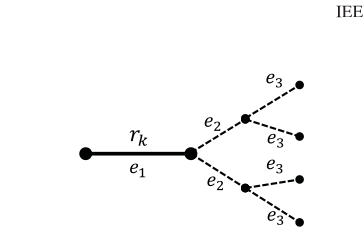
\includegraphics[]{figures/prediction_tree_omm.png}
    \caption{Contoh \textit{prediction} tree dari algoritma OMM-MHT (diadaptasi dari~\cite{Taguchi2019}).}
    \label{fig:prediction-tree-omm}
\end{figure}




\begin{algorithm}
\caption{Online Map-Matching dengan menggunakan Multi Hypothesis Technique (\cite{Taguchi2019})} 
\label{alg:omm-mht}
\resizebox{\textwidth}{!}{%
\begin{minipage}{\textwidth}
\scriptsize
\begin{algorithmic}[1]
\setstretch{0.9}
    \Procedure{OnlineMapMatchingMHT}{$G(V,E),g_{1:k},\Delta t_{1:k}$}
        \State $C \gets \{c\mid c.w=c.e.l, c.e \in E, dist(g_1,c.e)<L_C\}$
        \State $\overline{v} \gets g_1.v$
        \State $\sigma_v \gets \sigma_v$
        \For {$k=1 \textbf{ to }K$}
            \If {$k>1$}
                \State $C_{new} \gets \emptyset$
                \For {$\textbf{all } c \in C$} \Comment{prediksi}
                    \State $\tau \gets \{c.e\}$
                    \State $p_\tau\gets 1$ \Comment{menghitung $p(\tau)$}
                    \State $h_{pre} \gets 1$
                    \State $C_{new} \leftarrow$ \Call{Recur}{$C_{new},c.w,\tau,p_\tau,\overline{v},\sigma_v,\Delta t_{k-1}, h_{pre}$} \Comment{\textit{produce} \textit{candidates} baru yang dapat dilewati }
                \EndFor
                \State $C\leftarrow C_{new}$
                \State $\overline{v},\sigma_v\leftarrow KalmanFilter(\overline{v},\sigma_v,g_k.v)$
            \EndIf

            \For{$\textbf{all }c\in C$} \Comment{filtering}
                \State $c.w\leftarrow \frac{c.w\cdot ObservationProb(g_k,c)}{\sum_{c'\in C}c'.w\cdot ObservationProb(g_k,c')}$ \Comment{menghitung \textit{posterior probability} $p(r_{k}\mid g_{1:k})$ }
            \EndFor
            \State $\{c\mid c\in C, c.w>L_u\}$ \Comment{\textit{filter candidate} yang memiliki bobot $w> L_u$ }
            \State $r_k\leftarrow (\arg \max_{c\in C} c.w).e$
            \State \textbf{output } $r_k$
        \EndFor
    \EndProcedure

    \Procedure{Recur}{$C_{new},w,\tau,p_\tau,\overline{v},\sigma_v,\Delta t_{k-1}, \text{ dan } h_{pre}$}
        \State $h_{new}\leftarrow h(\tau,\overline{v},\sigma_v,\Delta t_{k-1})$ \Comment{menghitung $h(\tau_{1:n},\overline{v}_k,\sigma_{v,k},\Delta t_k)$}
        \If {$w \cdot p_\tau \cdot h_{new}>L_p$}
            \State $\mathcal{E}_{next} \gets \{e_{next}\mid e_{next}\in E, e_{next}.start=\tau.last.end\}$
            \For {$\textbf{all } e_{next}\in \mathcal{E}_{next}$}
                \State $\tau'\gets \{\tau\rightarrow\ e_{next}\}$
                \State $p_{\tau}' \gets p_\tau \cdot p(\tau.last\rightarrow e_{next})$ \Comment{menghitung probabilitas $p(e_{\tau.last}\rightarrow e_{next})$}
                \State $h'_{pre}\gets h_{new}$ \Comment{menghitung $h(\tau_{1:n-1},\overline{v}_k,\sigma_{v,k},\Delta t_k)$}
                \State $C_{new}\gets Recur(C_{new},w,\tau',p_{\tau}',\overline{v},\sigma_v,\Delta t_{k-1}, h'_{pre})$
            \EndFor
        \EndIf 
        \State $w' \gets w\cdot p_{\tau}\cdot (h_{pre}-h_{new})$ \Comment{menghitung  $p(r_{k}\mid r_{k-1})\ p(r_{k-1}\mid g_{{1:k-1}})$ }
        \State $c_{new}\gets C_{new}.Find(c_{new}\mid c_{new}.e=\tau .last)$
        \If{$c_{new}\neq null$}
            \State $c_{new}.w=c_{new}.w+w'$ \Comment{jumlahkan bobot dari \textit{states} yang diwakili > 1 kandidat yang sama untuk hitung \textit{prior}}
        \Else 
            \State $C_{new}\gets C_{new}\cup (\tau.last, w')$
        \EndIf
        \State \textbf{return} $C_{new}$
    \EndProcedure
        
    \Procedure{KalmanFilter}{$\overline{v}, \sigma_v, g_k.v$}
        \State $\overline{v}_{k}=\overline{v}_{k-1}$ \Comment{prediction}
        \State $\sigma_{v,k}=\sqrt{\sigma^2_{v,k-1}+ \sigma^2_{a}\Delta t^2_{k-1}}$
        \State $\overline{v} = \frac{\sigma_v^2 \overline{v}_{k}+\sigma^2_{v,k} g_k.v} {\sigma_v^2+\sigma_{v,k}^2}$\Comment{filtering}
        \State $\sigma_{v,k} =\sqrt{(\sigma^{-2}_v + \sigma^{-2}_{v,k})^{-1}}$
    \EndProcedure
\end{algorithmic}
\end{minipage}%
}
\end{algorithm}


    \section{Traffic Forecasting Dengan Menggunakan Multivariate Time-Series Graph Neural Network}
    \label{mtgnn-section}
    \subsection{Formulasi Masalah}
\label{subsec:traffic-forecasting-problem-formulation}
Diberikan sekuens data pengamatan lalu lintas sejumlah $M$ \textit{time steps} $\textbf{X}=\{x_{t-M+1},x_{t-M+2},\ldots,x_{t} \}, \ x_t\in \mathbb{R}^N$. $x_t$ adalah vektor kecepatan dari sejumlah $N$ segmen jalan pada waktu $t$. Tujuan prediksi kecepatan lalu lintas adalah memprediksi sekuens nilai dari $Y=\{x_{t+1},x_{t+2},\ldots,x_{t+Q}\}$. Graf jaringan jalan $G=(V,E)$ terdiri dari himpunan simpul $V$ yang berjumlah $N$ simpul  dan himpunan sisi $E$. Misalkan $v\in V$ adalah simpul dan $e=(v,u)\in E$ adalah sisi yang menghubungkan $v$ dengan $u$. $N(v)=\{u\in V\mid (v,u)\in E\}$ adalah tetangga dari simpul $v$. Matriks $adjacency$ $A\in \mathbb{R}^{N\times N}$ adalah representasi matematis dari graf, dengan $A_{ij}=c>0$ jika $(v_i,v_j)\in E$ dan $A_{ij}=0$ jika $(v_i,v_j)\notin E$. Simpul adalah stasiun pemantau lalu lintas dan sisi menunjukkan keterhubungan antar stasiun.

\subsection{Arsitektur Multivariate Time-Series Graph Neural Network (MTGNN)}
\label{subsec:traffic-forecasting-mtgnn-architecture}
Arsitektur dari MTGNN terdiri dari, \textit{graph learning layer}, sejumlah $m$ \textit{graph convolution layer}, sejumlah $m$ \textit{temporal convolution layer}, dan sebuah \textit{output layer}. \textit{Graph learning layer} mempelajari matriks \textit{adjacency} graf secara adaptif untuk menangkap hubungan tersembunyi di antara data \textit{traffic time series} tanpa perlu menentukan struktur graf secara eksplisit (\cite{Wu2020}). \textit{Graph learning layer} didefinisikan dengan:

\begin{align}
    \mathbf{M}_1 &= \tanh(\alpha \mathbf{E}_1 \mathbf{\Theta_1})\\
    \mathbf{M}_2 &= \tanh(\alpha \mathbf{E}_1 \mathbf{\Theta_1})\\
    \mathbf{A} &= \mathrm{ReLU}\bigl(\tanh\bigl(\alpha(\mathbf{M}_1\mathbf{M}_2^{T}-\mathbf{M}_2\mathbf{M}_1^{T})\bigr)\bigr) \\ 
    i \; &= \; 1,2,\ldots,N \\
   \hspace{2em}  \mathbf{idx} &= \mathrm{argtopk}(\mathbf{A}[i,:])\\
     \mathbf{A}[i,-\mathbf{idx}] &= 0, 
\end{align}

Dimana $\mathbf{E}_1,\mathbf{E}_2\in \mathbb{R}^{N\times d_e}$ adalah \textit{node embeddings} yang dinisialisasi secara acak dan dapat dipelajari selama pelatihan. $\mathbf{\Theta_1},\mathbf{\Theta_2}\in \mathbb{R}^{d_e \times d_t}$ adalah parameter model, dan $\alpha$ adalah \textit{hyperparameter} untuk mengontrol tingkat saturasi dari fungsi aktivasi, dan $argtopk(\cdot)$ mengembalikan indeks dari sejumlah k nilai terbesar dari vektor.\textit{ Graf learning layer} mengekstrak hubungan \textit{uni-directional} dari setiap simpul. Hal ini disebabkan karena ketika $A_{vu}>0$, maka nilai sisi terbaliknya $A_{uv}=0$. 
\begin{align}
    T_{uv}=tanh(\alpha(M_{1u}M_{2v}^T-M_{2u}M_{1v}^T))\\
    T_{vu}=tanh(\alpha(M_{1v}M_{2u}^T-M_{2v}M_{1u}^T))\\
    T_{vu}=-T_{uv}\\
    A_{vu}=Relu(-T_{uv})=\max (0,-T_{uv})=0
\end{align}

Persamaan (3.19)-(3.20) membuat matriks $adjacency$ graf menjadi \textit{sparse} dengan cara menetapkan nilai $adjacency$ tetangga-tetangga yang tidak terlalu relevan (tidak termasuk \textit{top} k nilai terbesar dari vektor $\mathbf{A[i,:]}$) dari setiap simpul $i$ sama dengan nol.

\textit{Graph Convolution layer} mempelajari ketergantungan spasial menggunakan dua \textit{mix-hop }\textit{propagation layers} untuk memproses informasi aliran lalu lintas masuk dan keluar yang melewati setiap simpul secara terpisah. Gambar~\ref{fig:gc-layer} menunjukkan arsitktur dari \textit{graph convolution layer}. \textit{Mix-hop propagation layer} dapat mempelajari kombinasi linear fitur-fitur dari simpul-simpul tetangga yang memiliki jarak beberapa \textit{hop} dari suatu simpul. \textit{Mix-hop propagation layer} terdiri dari tahapan \textit{information propagation} dan tahapan \textit{information selection}. Tahapan \textit{information propagation} menyebarkan informasi simpul-simpul mengikuti struktur graf yang sudah dipelajari. Arsiktektur mix-hop propagation layer ditampilkan pada Gambar~\ref{fig:mixhop-layer}. Tahapan \textit{information propagation} didefinisikan dengan:
\begin{equation}
    \mathbf{H}^{(k)}=\beta \mathbf{H}_{in}+(1-\beta ) \tilde{\mathbf{A}} \mathbf{H}_{(k-1)}
\end{equation}


\begin{figure}[H]
    \centering
    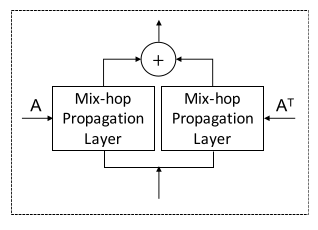
\includegraphics[]{figures/gc_layer.png}
    \caption{Arsitektur dari Graph Convolution Layer}
    \label{fig:gc-layer}
\end{figure}



\begin{figure}[H]
    \centering
    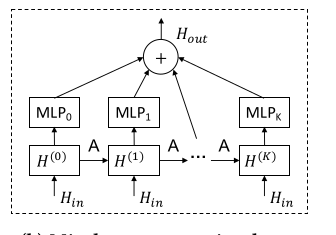
\includegraphics[]{figures/mix_hop.png}
    \caption{Arsitektur dari Mix-hop Propagation Layer}
    \label{fig:mixhop-layer}
\end{figure}


Dimana $\beta$ adalah \textit{hyperparameter} yang mengatur rasio antara fitur \textit{hidden states}  pada \textit{layer} sebelumnya dengan informasi \textit{hidden states} pada \textit{hop} sebelumnya $(k-1)$ yang akan dipertahankan pada \textit{hidden states} pada \textit{hop} $k$. Tahapan \textit{information selection} menggabungkan berbagai fitur \textit{hidden states} pada setiap \textit{hop} dengan memberikan bobot $\mathbf{W}^{k}$ pada setiap fitur. Tahapan \textit{information selection} didefinisikan dengan:
\begin{equation}
    \mathbf{H}_{out} = \sum_{i=0}^{K}\mathbf{H}^{(k)}\mathbf{W}^{(k)}
\end{equation}

Temporal Convolution Layer mengekstrak  fitur temporal dari data \textit{time series} lalu lintas melalui serangkaian operasi \textit{1D convolutional filters}. Arsitektur dari temporal Convolutional layer ditunjukkan pada Gambar~\ref{fig:tc-layer}. Temporal Convolution Layer terdiri dari dua \textit{dilated inception layers}. Kedua \textit{dilated inception layer} tersebut menjadi input dari Gated Linear Unit (GLU) dengan satu input memiliki fungsi aktivasi tangen hiperbolik dan satunya lagi memiliki fungsi aktivasi \textit{sigmoid}. GLU berfungsi sebagai gerbang yang mengontrol banyaknya informasi hasil dari \textit{dilated convolution} yang dapat diteruskan pada \textit{layer} selanjutnya. \textit{Dilated convolution layer} menjalankan beberapa \textit{dilated convolution} dengan setiap \textit{convolution} memliki ukuran kernel yang berbeda-beda. Hal ini membuat model dapat mempelajari pola temporal dari data dengan berbagai rentang waktu (\textit{short-term}, \textit{long-term}, dan \textit{medium-term}) dan membuat model mampu mengaproksimasi stuktur \textit{optimal network topology} (\cite{Wu2020}). \textit{Dilated convoluton layer} memberikan jarak pada setiap bobot \textit{convolution kernel} dan membuat ukuran \textit{reception field } dari model meningkat secara eksponensial. \textit{Dilated convolution layer} membuat model mampu menangkap pola sekuens yang lebih panjang. \textit{Dilated convolution operation} pada setiap kernel didefinisikan dengan:
\begin{equation}
    \mathbf{z} \star \mathbf{f}_{1\times k}(t)  =b+\sum_{j=0}^{k-1}  \mathbf{f_{1\times k}}[j] \mathbf{z}[t-d\times j]
\end{equation}

\textit{Dilated convolution layer} didefinisikan dengan:
\begin{equation}
    z_{out}= concat(\mathbf{z} \star \mathbf{f}_{1\times 2}(t), \mathbf{z} \star \mathbf{f}_{1\times 3}(t), \mathbf{z} \star \mathbf{f}_{1\times 6}(t), \mathbf{z} \star \mathbf{f}_{1\times 7}(t))
\end{equation}

\begin{figure}[H]
    \centering
    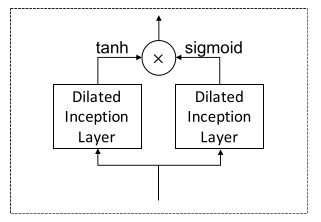
\includegraphics[]{figures/tc_layer.png}
    \caption{Arsitektur dari Temporal Convolution Layer}
    \label{fig:tc-layer}
\end{figure}

Penulis menambahkan \textit{Residual Connection Layer} yang meneruskan input dari Temporal Convolution layer ke output dari Graph Convolution Layer  dan mnambahkan \textit{skip connections} yang meneruskan output dari setiap Temporal Convolution Layer ke output layer. Hal ini bertujuan untuk mencegah terjadinya \textit{vanishing gradient problem} pada saat \textit{training} model. Output layer tediri dari dua 1x1 \textit{convolution layer} yang memetakan input ke dimensi output $Q$. Dimana $Q$ adalah jumlah \textit{step} prediksi yang diinginkan. Arsitektur dari Multivariate Time-Series Graph Neural Network ditunjukkan pada Gambar~\ref{fig:mtgnn-architecture}. MTGNN menggunakan \textit{L2 loss function}/\textit{mean squared error}  untuk mengukur performa dari model. MTGNN dilatih dengan menggunakan \textit{curriculum learning}, dimana algoritma dimulai dengan memprediksi satu \textit{time step}. Seiring bertambahnya iterasi, panjang prediksi model meningkat secara bertahap.\textit{Pseudocode} untuk  \textit{curiculum learning} ditunjukkan pada Algoritma~\ref{alg:mtgnn-learning}.


\begin{algorithm}
\caption{Curiculum Learning dengan input \textit{dataset} $O$, model $f(\cdot)$, parameter model $\Theta$, \textit{learning rate} $\gamma$, \textit{batch size} $b$, \textit{step size} $s$, \textit{split size} $m$}
\label{alg:mtgnn-learning}
\resizebox{\textwidth}{!}{%
\begin{minipage}{\textwidth}
\scriptsize
\begin{algorithmic}[1]
\setstretch{0.9}
    \Procedure{CuriculumLearning}{$O, f(\cdot), V, \Theta, \gamma,  b, s, m$}
        \State $iter\gets 1, r \gets 1$
        \While{$\textbf{until convergence}$}
            \State $\text{sampel satu batch }  \mathcal{X}\in \mathbb{R}^{b\times T \times N \times D}, \mathcal{Y}^{b\times T' \times N} \text{ dari } O $
            \State $\text{random split } V \text{ menjadi } m \text{ grup } \cup_{i=1}^{m}V_i=V$
            \If {$iter \% s=0 \text{ and }  r\leq T'$}
                \State $r \gets r+1$
            \EndIf
            \For {$i =1 \to m$}
                \State $\text{hitung }  \hat{\mathcal{Y}} \gets f(\mathcal{X}[:,:,id(V_i),:], \Theta)$
                \State $\text{hitung } L\gets MSE(\hat{\mathcal{Y}}[:,:r,:], \mathcal{Y}[:,:r,id(V_i)])$
                \State $\text{update parameter } \Theta \text{ berdasarkan \textit{gradient} dari \textit{loss function} dan \textit{learning rate }} \gamma$ 
            \EndFor 
            \State $iter \gets iter+1$
            \EndWhile 
    \EndProcedure
\end{algorithmic}
\end{minipage}%
}
\end{algorithm}

\begin{figure}[H]
    \centering
    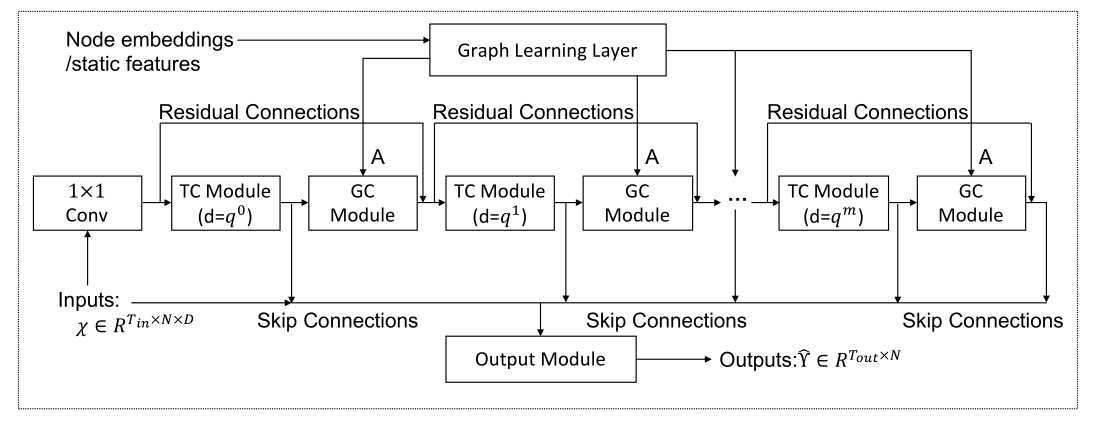
\includegraphics[width=0.9\textwidth]{figures/mtgnn.png}
    \caption{Arsitektur dari Multivariate Time-Series Graph Neural Network}
    \label{fig:mtgnn-architecture}
\end{figure}

    
     \section{Pencarian Rute Alternative Dengan Metode Heuristik Admissible Paths}
    \label{alternative-routes}
    Untuk mencari rute alternatif, \cite{Abraham2010} memperkenalkan metode heuristik \textit{admissible paths} Adimissble Paths untuk mencari rute alternatif pada jaringan jalan. Secara intuitif, rute alternatif berbeda secara signifikan dari rute tercepat $Opt$, tetapi rute tersebut masuk akal dan tidak lebih jauh daripada rute $Opt$ \cite{Abraham2010}. Diberikan semua kemungkinan rute $P$ dari simpul $s$ ke simpul $t$, rute $P$ disebut sebagai \textit{admissible alternative} jika memenuhi sifat-sifat berikut:
\begin{enumerate}
    \item \textit{Limited sharing}. Penjumlahan \textit{travel time} dari sisi-sisi yang muncul pada kedua rute \textit{Opt} dan rute \textit{P} ($\sigma(v)$) kurang dari $\gamma \cdot dist(s,t), 0 \leq \gamma \leq 1$.
    \item \textit{Local optimality}. Setiap subrute dari $P$ memiliki \textit{travel time} yang lebih kecil dari $\alpha \cdot dist(s,t), 0<\alpha<1$.
    \item \textit{Bounded stretch}. Setiap pasang simpul $u,v\in P$, berlaku $l(P_{uv})< (1+\epsilon)\cdot dist(u,v), \epsilon \geq 1$. 
\end{enumerate}

Agar metode \textit{admissible paths} bisa diintegrasikan dengan Time-Dependent Customizable Route Planning (TD-CRP), diperlukan sedikit modifikasi pada algoritma kueri. Karena metode \textit{admissible paths} menentukan kandidat rute-rute alternatif dari himpunan rute $s-v-t$, dimana $v$ adalah simpul yang dikunjungi oleh \textit{forward search} dan \textit{backward search}, kueri TD-CRP perlu dibuat \textit{bidirectional}. \textit{Upper} dan \textit{lower bound} dari \textit{minimum travel time } dari simpul $s$ ke $t$ didefinisikan dengan:
\begin{align}
    Max_{G}(s,t)=\min \{ \sum_{i=1}^{k-1} \max f_i \mid (v_1 \rightarrow_{f_1} \ldots \rightarrow_{f_{k-1}} v_k ) \text{ adalah rute dari simpul } s \text{ ke simpul } t \} \\ 
    Min_{G}(s,t)=\min \{ \sum_{i=1}^{k-1} \min f_i \mid (v_1 \rightarrow_{f_1} \ldots \rightarrow_{f_{k-1}} v_k ) \text{ adalah rute dari simpul } s \text{ ke simpul } t \} \\
    Min_{G}(s,t)\leq TTP_G(s,t)(\tau)\leq Max_G(s,t) \text{ untuk semua } \tau\in \mathbb{R}
\end{align}



\begin{algorithm}
\caption{BDTDDijkstra menghitung kandidat \textit{via nodes} $X=\{\ v\in V| v \text{ is visited by forward and backward search} \}\subseteq V$. \textit{Backward search} menghitung label $[q[u], r[u]]=[Min_G(t,u),Max(t,u)]$ untuk semua $u$ yang dikunjungi \textit{backward search}.} 
\label{alg:bidirectional-td-dijkstra-crp}
\resizebox{\textwidth}{!}{%
\begin{minipage}{\textwidth}
\scriptsize
\begin{algorithmic}[1]
\setstretch{0.9}
    \Procedure{BDTDDijkstra}{$s,t:V, \tau_0: \mathbb{R}$}: $(Set, \mathbb{R}, Set, Set, Set, Set)$
    \State $\tau[u]=\infty, \ u\in v, \ \tau[s]=\tau_0$ \Comment{\textit{node time travel label}}
    \State $[q[u],r[u]]=[\infty, \infty], \ u\in V, \ [q[t], t[t]]=[0,0]$ \Comment{\textit{Lower bound } dan \textit{upper Bound minimum travel time label}}
    \State $p_s[u]=\perp, p_t[u]=\emptyset, \ u\in V $
    \State $B=\infty, \ d=t$ \Comment{arah pencarian (\textit{forwardSearch} atau \textit{backwardSearch})}
    \State $X=\emptyset$
    \State $Q_s=\{(s_, sEntryPos, \tau_0)\}, \ Q_t=\{(t, tEntryPos,0)\}$
    \State $overlayQ_s=\emptyset, \ overlayQ_t=\emptyset $
    \While{$(Q_S \neq \emptyset \textbf{ or } Q_t\neq \emptyset) \textbf{ and }  \min \{Q_s.min(), overlayQ_s.min()\} + \min \{Q_t.min(), overlayQ_t.min()\}\leq (1+\epsilon) B$}
        \State $minG = \min \{ Q_s, Q_t \}$
        \State $minOverlayG = \min \{ overlayQ_s, overlayQ_t \}$
        \If{$ minG < minOverlayG$}
            \If {$Q_{\neg d}\neq \emptyset $}
                \State $d=\neg d$ 
            \EndIf 
            \State $(u, uEntryPos)=Q_d.deleteMin()$
            \If{$B<\infty \textbf{ and } \tau[u] + q[u] \leq B $}
                \State $X= X \cup \{(u, \tau[u]+r[u])\}$ \Comment{simpul $u$ dikunjungi oleh \textit{forward search} dan \textit{backward search}}
            \EndIf 
    
            \State $B= \min \{B, \ \tau[u]+r[u]\}$
            \For {$(u \rightarrow_f v, turnCost_{uv}) \in E_d $}
                \If{$d=s$}
                    \State \Call{tdRelaxCRP}{$u\rightarrow_f,v,v,u,uEntryPos,\tau,p_s,Q_s,overlayQ_s,turnCost_{uv}$}
                \Else 
                    \State \Call{intervalRelaxCRP}{$u,v,[q[u]+min f, \ r[u]+max f], q,r,p_t, Q_t,overlayQ_t$}
                \EndIf 
            \EndFor 
        \Else 
            \If {$overlayQ_{\neg d}\neq \emptyset $}
                \State $d=\neg d$
            \EndIf 
            \State $u=overlayQ_d.deleteMin()$
            \If{$B<\infty \textbf{ and } \tau[u] + q[u] \leq B $}
                \State $X= X \cup \{(u,\tau[u]+r[u])\}$ \Comment{simpul $u$ dikunjungi oleh \textit{forward search} dan \textit{backward search}}
            \EndIf 
    
            
            \State $B= \min \{B, \ \tau[u]+r[u]\}$
            \State $l_{st}(u)=\min\{MSD(PV(s), PV(u)), MSD(PV(t), PV(u))\}$
            \For {$u \rightarrow_{f_{shortcut\_uv}} v \in E_{d,C^{l_{st}(u)}} $}
                \If{$d=s$}
                    \State \Call{tdRelaxOverlayCRP}{$u\rightarrow_{f_{shortcut\_uv}}v,v,u, uEntryPoint,\tau,p_s,Q_s,overlayQ_s$}
                \Else 
                    \State \Call{intervalRelaxCRP}{$u,v,uEntryPoint,[q[u]+min f_{shortcut\_uv}, \ r[u]+max f_{shortcut\_uv}], q,r,p_t, Q_t,overlayQ_t$}
                \EndIf 
            \EndFor 
        \EndIf 
        
        
    \EndWhile
    \State \textbf{return} $\mathbf{X}, B, p_s, p_t, \tau, r$
    \EndProcedure
\end{algorithmic}
\end{minipage}%
}
\end{algorithm}


\begin{algorithm}
\caption{intervalRelaxCRP memperbarui label $[q[v], r[v]]=[Min_G(t,v),Max_G(t,v)]$} 
\label{alg:intervalRelaxCRP}
\resizebox{\textwidth}{!}{%
\begin{minipage}{\textwidth}
\scriptsize
\begin{algorithmic}[1]
\setstretch{0.9}
    \Procedure{intervalRelaxCRP}{$u,v, uEntryPoint, \ [q_{new}, r_{new}], q,r, p, Q, overlayQ, turnCost_{uv}$}
    \If{$q_{new}>r[v]$} 
        \State \textbf{return} \Comment{nilai \textit{Lowerbound travel time} baru dari $v$ melebihi \textit{Upperbound travel time} lama dari $v$}
    \EndIf 
    \If{$r_{new}<q[v]$}
        \State $p[v]=\emptyset$ \Comment{nilai \textit{Upperbound travel time} baru dari $v$ kurang dari \textit{Lowerbound travel time} lama dari $v$}
    \EndIf
    \State $p[v]= u\cup p[v]$
    \If{$q_{new}\geq q[v] \textbf{ and }r_{new} \geq r[v]$}
        \State \textbf{return} \Comment{nilai \textit{lowerbound travel time} dan \textit{upperbound travel time} baru melebihi nilai lama}
    \EndIf 

    \State $l_{st}(v)=min\{MSD(PV(s), PV(v)), MSD(PV(t), PV(v))\}$
    \If{$l_{st}(v) =0$ }
        \State $[q[v], r[v]]=[\min\{q[v], q_{new}+turnCost_{uv}\}, \min \{r[v], r_{new}+turnCost_{uv}\}]$
        \If{$v\notin Q$}
            \State $Q.insert(v, q[v])$
        \Else 
            \State $Q.decreaseKey(v, q[v])$
        \EndIf 
    \Else 
        \State $vOverlay = GetOverlayVertex(v, uEntryPoint)$
        \State $[q[vOverlay], r[vOverlay]]=[\min\{q[vOverlay], q_{new}+turnCost_{uv}\}, \min \{r[vOverlay], r_{new}+turnCost_{uv}\}]$
        \If{$vOverlay\notin overlayQ$}
            \State $overlayQ.insert(vOverlay, q[vOverlay])$
        \Else 
            \State $overlayQ.decreaseKey(vOverlay, q[vOverlay])$
        \EndIf 
    \EndIf 
    \EndProcedure

    
\end{algorithmic}
\end{minipage}%
}
\end{algorithm}

Algoritma pencarian rute alternatif dimulai dari menjalankan $BDTDDijkstra$ untuk mendapatkan kandidat \textit{via nodes} $v\in V$. Algoritma $BDTDDijkstra$ terinspirasi dari kueri \textit{bidirectional} pada Time-Dependent Contraction Hierarchies yang diperkenalkan pada penelitian oleh \cite{Veit2013}. Kueri Bidirectional Time-Dependent Dijkstra untuk Customizable Route Plannning ditunjukkan pada Algoritma~\ref{alg:bidirectional-td-dijkstra-crp}. Dalam \textit{bidirectional search}, memperbarui \cite{Veit2013} \textit{upperbound} $B$, jika simpul $u$ yang baru saja di \textit{settled} sudah dikunjungi pada \textit{forward search} dan \textit{backward search}. $B$ adalah \textit{upperbound} dari $EA_G(s,t,\tau_0)$ dengan nilai awal $\infty$. \textit{Backward search} adalah aproksimasi dari $ProfileSearch$ dan menghitung label $[q[u], r[u]]=[Min_G(t,u), Max_G(t,u)]$ untuk semua simpul $u$ yang dikunjungi pada kedua \textit{search}. Simpul $v$ yang dikunjungi pada kedua \textit{search} termasuk dalam \textit{candidate/via nodes} $X$. \textit{Via node} $u$ adalah simpul $u$ yang memiliki $\tau[u] + r[u] < \infty$. \textit{Forward search} menjalankan Algoritma~\ref{alg:td-dijkstra-crp}. Algoritma $BDTDDijkstra$ menghitung \textit{upperbound} $B$ yang merupakan penjumlahan dari label \textit{minimum departure time} tentatif \textit{forward} search $\tau[u]\in \Pi$ dan \textit{upperbound minimum travel time} $r[u]\in \mathbb{R}$ dari \textit{backward search} dengan \textit{source} $t$, untuk semua simpul $u$ yang dikunjungi pada kedua pencarian. Dengan kata lain, untuk simpul-simpul $u$ yang termasuk ke dalam \textit{via nodes} $X$, kita bisa melakukan perjalanan dari $s$ ke $t$ melalui $u$ dengan mengunjungi sisi-sisi yang dikunjungi \textit{forward search} yang optimal (menghasilkan \textit{minimum travel time } untuk waktu keberangkatan $\tau_0$) dan mengunjungi sisi-sisi yang optimal (memiliki nilai minimal dari \textit{upper bound} TTF dari sisi) yang dikunjungi backward search. Untuk setiap \textit{via node} $v$, cari rute tercepat $s-v$ dan $v-t$ dengan menggunakan $TDDijkstraCRP$ yang jika digabung akan menghasilkan rute $P_v$ dengan \textit{time travel} $l(v)$. Untuk semua kemungkinan rute $P$ dari $s$ ke $t$, $P_v$ memiliki nilai \textit{stretch} yang sangat kecil, atau dengan kata lain $l(P_v)\leq l(P)$ (\cite{Abraham2010}). Hitung skor $f(v)=2l(v)+\sigma(v)-pl(v)$. Dimana $l(v)$ adalah \textit{travel time } tentatif optimal dari $v$ ( $(\tau[v]+r[v])-\tau_0$) saat menjalankan $BDTDDijkstra$. $\sigma(v)$ adalah penjumlahan \textit{travel time} dari sisi-sisi yang muncul pada kedua rute \textit{Opt} dan rute $P_v$. $pl(v)$ adalah plateau dari simpul $v$. Plateau $pl(v)$ dapat dicari dengan membuat subrute $P_{plateau\_v}\subseteq Opt$ yang berisi simpul-simpul $u\in P_{plateau\_v}$ dengan $dist(s,u)+dist(u,t)=l(v)$, $pl(v)$ dihitung dengan menjumlahkan bobot \textit{time travel} dari sisi-sisi $P_{plateau\_v}$. Untuk memastikan kandidat rute alternatif memenuhi kriteria \textit{admissible paths}, kita membuang kandidat yang memiliki: $l(v)\geq (1+\epsilon)\cdot l(Opt), \sigma(v)\geq\gamma \cdot l(Opt), \text{ atau } pl(v)\leq \alpha \cdot l(Opt)$. Rute-rute alternatif yang dikembalikan adalah kandidat-kandidat yang memiliki $f(v)$ terkecil. Algortima pencarian rute alternatif \textit{admissible paths} ditunjukkan pada Algoritma~\ref{alg:alternative-routes}. Algoritma ini memiliki kompleksitas waktu $O(C_v\cdot (E_1+U_1\log U_1+B^{2}+B \log B))$, dimana $C_v$ adalah jumlah \textit{via node} $v$ yang ditemukan oleh algoritma $BDTDDijkstra$.


\begin{algorithm}
\caption{findAlternativeRoutes mengembalikan sejumlah $k$ rute alternatif terbaik} 
\label{alg:alternative-routes}
\resizebox{\textwidth}{!}{%
\begin{minipage}{\textwidth}
\scriptsize
\begin{algorithmic}[1]
\setstretch{0.9}
    \Procedure{findAlternativeRoutes}{$s,t: V, \tau_0: \mathbb{R}, k: \mathbb{Z}^+$}: $Set$
        \State $(l_{Opt}, shortestPath, \cdot, \cdot) =$\Call{tdDijkstraCRP}{$s,t, \tau_0$} 
        \State $(\mathbf{X}, \cdot, p_{sbd}, p_{tbd}, \tau_{bd}, r)=$\Call{BDTDDijkstra}{$s,t, \tau_0$}
        \State $potentialCandidates = \emptyset$
        \Procedure{calculatePlateau}{$\tau_{sbd},\tau_{tbd},v, l_v, p_{s}, p_t, \tau_0$}: $\mathbb{R}$
             \State $plateau = 0$
             \State $u = v$
             \While{$u \neq \perp$} \Comment{backtrack}
                    \If{$u\in p_t \textbf{ and } (\tau_{sbd}[u]-\tau_0)+ \tau_{tbd}[u] = l_v $} \Comment{$dist(s,u)+dist(u,t)=l(v)$}
                        \State $cost_{uf}= (\tau_{sbd}[u]-\tau_0)-(\tau_{sbd}[p_{s}[u]]-\tau_0)$
                        \State $ plateau = plateau + cost_{uf} $
                        \State $u = p_{s}[u]$
                    \EndIf
             \EndWhile
             \State $u = v$
             \While{$u \neq \perp$} \Comment{backtrack}
                    \If{$u\in p_s \textbf{ and } (\tau_{sbd}[u]-\tau_0)+ \tau_{tbd}[u] = l_v $} \Comment{$dist(s,u)+dist(u,t)=l(v)$}
                        \State $cost_{ub}= \tau_{tbd}[u]-\tau_{tbd}[p_{t}[u]]$
                        \State $ plateau = plateau +  cost_{ub} $
                        \State $u = p_{t}[u]$
                    \EndIf
             \EndWhile
             \State \textbf{return} $plateau$
        \EndProcedure
    
        \Procedure{calculatedistanceShare}{$Opt, P$}: $\mathbb{R}$
            \State $distanceShare= 0$
            \For{$p\in P$}
                \If {$p \in Opt$}
                    \State $distanceShare = distanceShare + p.weight$ 
                \EndIf 
            \EndFor
            \State \textbf{return} $distanceShare$
        \EndProcedure
        \For {$candidate \in X$}
            \State $(svTimeTravel, shortestPath, p_s, \tau_{sv}) = $\Call{tdDijkstraCRP}{$s,candidate.node, \tau_0$} 
            \State $(vtTimeTravel, shortestPath, p_t, \tau_{vt}) = $\Call{tdDijkstraCRP}{$candidate.node, t, \tau_0$} 
            \State $l_v=svTimeTravel+vtTimeTravel$
            \If{$l_v \geq (1+\epsilon)\cdot l_{Opt} $}
                \State $\textbf{continue}$
            \EndIf

            
            \State $edgesSV=$\Call{backtrack}{$p_s, candiate.node$}
            \State $edgesVT=$\Call{backtrack}{$p_t, candiate.node$}
            \State $\sigma_v=$\Call{calculatedistanceShare}{$shortestPath, edgesSV \cup edgesVT$}
            \If{$\sigma_v\geq \gamma \cdot l_{Opt}$}
                \State \textbf{continue} 
            \EndIf
            \State $pl_v=$\Call{calculatePlateau}{$\tau_{bd},r,candidate.node,  l_v, p_{sbd}, p_{tbd}, \tau_0$}
            \If{$pl_v \leq \alpha \cdot l_{Opt}$}
                \State \textbf{continue} 
            \EndIf
            \State $f_v=2l_v+\sigma_v-pl_v$
            \State $potentialCandidates  = potentialCandidates \cup \{candidate.node\}$
        \EndFor
        \State $sortedCandidates=$\Call{sort}{$potentialCandidates$}
        \State \textbf{return} $sortedCandidates[:k]$
    \EndProcedure

    
\end{algorithmic}
\end{minipage}%
}
\end{algorithm}





    \section{Mempartisi Graf Jaringan Jalan Dengan Algoritma Inertial Flow}
    \label{alternative-routes}
    Diberikan graf tidak berarah $G=(V,E)$,  \textit{graph partitioning} adalah proses membagi himpunan simpul $V$ menjadi beberapa subset $V_0,V_1,\ldots V_{k-1}$ yang saling \textit{disjoint} sedemikian hinggga setiap ukuran partisi-partisi $(V_i,E_i),i\in\{0,1,\ldots, K-1\}$ kurang lebih sama dan jumlah sisi-sisi batas $E(V_i,V_j)$ yang menghubungkan partisi $V_i$ dan $V_j$ ($i\neq j$) seminimal mungkin. Penulis menggunakan algoritma Inertial Flow yang diperkenalkan pada penelitian oleh \cite{Schild2015}. Algoritma Inertial Flow diawali dengan mengurutkan simpul-simpul berdasarkan \textit{latitude} dan \textit{longitude}. Setelah simpul-simpul terurutkan, algoritma kemudian menjalankan algoritma Dinic dengan \textit{unit-capacity} \cite{Dinitz2006} menggunakan sejumlah $k$ simpul awal sebagai \textit{sources} dan sejumlah $k$ simpul terakhir sebagai \textit{sinks} dari himpunan simpul yang telah diurutkan. Proses yang terdiri dari dua langkah ini diterapkan secara rekursif pada setiap partisi yang dihasilkan hingga ukuran partisi menjadi cukup kecil (ukuran partisi kurang dari \textit{threshold} $U$ yang kita tetapkan sendiri nilainya). Dari sejumlah $k$ simpul sebagai \textit{sources} dan sejumlah $k$ simpul sebagai \textit{sinks}, dibentuk sebuah \textit{artificial source} $s$ yang dihubungkan ke semua simpul \textit{sources} dengan sisi berbobot $\infty$, serta sebuah \textit{artificial sink} $t$ yang dihubungkan dari semua simpul \textit{sinks} dengan sisi berbobot $\infty$. Kedua simpul \textit{artificial} menjadi input dari algoritma Dinic. Pseudocode dari algoritma Inertial Flow ditunjukkan pada Algoritma~\ref{alg:inertial-flow}. Contoh hasil dari mempartisi graf jaringan jalan menggunakan algoritma Inertial Flow ditunjukkan pada Gambar~\ref{fig:inertial-flow}. Kompleksitas waktu dari algoritma Dinic adalah $O(N^2\cdot M)$ (\cite{Dinitz2006}),dimana $N$ adalah jumlah simpul dan $M$ adalah jumlah sisi. Kompleksitas waktu dari algoritma Inertial Flow adalah $O(N^2\cdot M)$ yang diberikan oleh relasi rekurens berikut:

\begin{align}
    T(N,M)&=N^2\cdot M \cdot C + T(N/2,M/2)+T(N/2,M/2) \notag \\
    &=N^2\cdot M \cdot C + 2T(N/2,M/2)  \notag \\
    &= N^2\cdot M \cdot C + \frac{ N^2}{2^2}\cdot M \cdot C + 2^2T(N/2^2,M/2^2)  \notag \\
    &= N^2\cdot M \cdot C + \frac{ N^2}{2^2}\cdot M   \cdot C + \frac{ N^2}{2^4}\cdot M \cdot C  + 2^3T(N/2^3,M/2^3)  \notag \\
    &= N^2\cdot M \cdot C + \frac{ N^2}{2^2}\cdot M \cdot C + \ldots + \frac{ N^2}{2^{2\cdot (k-1)}}\cdot M \cdot C  + 2^kT(N/2^k, M/2^k)  \notag \\
    & \text{(base case: $N/2^k = U, T(U,M/2^k)=1$)}  \notag \\ 
    &=\sum_{i=0}^{\log_2(N/U)-1} \frac{ N^2}{4^{i}}\cdot M \cdot C + \frac{N}{U}  \notag \\
    &\leq \sum_{i=0}^{\infty} \frac{ N^2}{4^i}\cdot M \cdot C+ \frac{N}{U}  \notag \\
    &= \frac{4}{3}\cdot N^2 \cdot M \cdot C \notag \\
    &=O(N^2\cdot M) \notag 
\end{align}


\begin{algorithm}
\caption{InertialFlow mengembalikan partisi-partisi dari graf $V_0,V_1,\ldots V_{k-1}$} 
\label{alg:inertial-flow}
\resizebox{\textwidth}{!}{%
\begin{minipage}{\textwidth}
\scriptsize
\begin{algorithmic}[1]
\setstretch{0.9}
\Procedure{InertialFlow}{$V, U$}
    \State $ partitionGraph \gets V $
    \State $Q \gets \emptyset : Queue$
    \State $Q.Enqueue(partitionGraph)$
    \State $partitions \gets \emptyset $
    \Procedure{computeDinic}{$currPartitionGraph$}
        \State $lines \gets \{ \{1,0\}, \{0,1\}, \{1,1\}, \{1,-1\}, \{-1,1\} \}$
        \For{$i = 0 \to 5$}
            \State $lines \gets lines \cup \{random(0,1), random(0,1) \}$
        \EndFor
        \State $bestpart_1 \gets \emptyset$
        \State $bestpart_2 \gets \emptyset$
        \State $bestCutEdgesCount \gets \infty$
        \For {$line \in lines$}
            \State $(sources,sinks) \gets $\Call{SortVerticesByLineProjection}{$line, currPartitionGraph$}
            \State $s,t \gets$ \Call{createArtificialSourceSink}{$sources,sinks$}
            \State $(cutEdges, part_1, part_2) \gets$ \Call{Dinic}{$s,t, currPartitionGraph$}
            \If{$cutEdges < bestCutEdgesCount$}
                \State $cutEdges \gets bestCutEdgesCount$
                \State $bestpart_1 \gets part_1$
                \State $bestpart_2 \gets part_2$
            \EndIf 
        \EndFor
        \State \textbf{return} $bestpart_1, bestpart_2$
    \EndProcedure
    \While{$Q \neq \emptyset $}
        \State $currPartitionGraph \gets Q.Dequeue()$
        \State $(part_1, part_2) \gets $\Call{computeDinic}{$currPartitionGraph$} 
        \If{$|part_1| > U$}
            \State $Q.Enqueue(part_1)$
        \Else 
            \State $partitions \gets partitions \cup \{part_1\}$
        \EndIf
        \If{$|part_2| > U$}
            \State $Q.Enqueue(part_2)$
        \Else 
            \State $partitions \gets partitions \cup \{part_2\}$
        \EndIf 
    \EndWhile
\EndProcedure

\end{algorithmic}
\end{minipage}%
}
\end{algorithm}



\begin{algorithm}
\caption{Dinic mengembalikan $(cutEdges, part_1, part_2)$} 
\label{alg:dinic}
\resizebox{\textwidth}{!}{%
\begin{minipage}{\textwidth}
\scriptsize
\begin{algorithmic}[1]
\setstretch{0.9}
\Procedure{Dinic}{$sources,sinks, currPartitionGraph$}
    \State $cutEdges \gets 0$
    \For{$e\in currPartitionGraph.E$}
        \State $e.capacity \gets 1 $ \Comment{\textit{unit-capacity} Dinic}
    \EndFor 
    \State $levels \gets \emptyset $
    \While{$true$}
        \If {\Call{bfsLevelGraph}{$s,t, currPartitionGraph, levels$} $=true$}
            \While{$true$}
                \State $flow \gets$ \Call{dfsAugmentPath}{$s,t, \infty, currPartitionGraph, levels$}
                \If {$flow = 0$}
                    \State \textbf{break}
                \EndIf
                \State $cutEdges \gets cutEdges + flow$
            \EndWhile 
        \Else 
            \State $part_1, part_2 \gets \emptyset$
            \For {$v \in currPartitionGraph.V$}
                \If {$levels[v] \neq \infty$}
                    \State $part_1 \gets part_1 \cup \{v\}$
                \Else 
                    \State $part_2 \gets part_2 \cup \{v\}$
                \EndIf
            \EndFor 
            \State \textbf{return} $(cutEdges, part_1, part_2)$
        \EndIf 
    \EndWhile 
\EndProcedure

\Procedure{bfsLevelGraph}{$s,t, currPartitionGraph, levels$}: $boolean$
    \For{$v\in currPartitionGraph.V$}
        \State $levels[v] \gets \infty $
    \EndFor 
    \State $Q \gets \emptyset : Queue$
    \State $Q.Enqueue(s)$
    \State $levels[s] \gets 0$
    \While {$Q \neq \emptyset$}
        \State $u \gets Q.Dequeue()$
        \State $level_u \gets levels[u]$
        \State $level \gets level_u +1 $
        \If {$u = t $}
            \State \textbf{break}
        \EndIf 
        \For {$e\in currPartitionGraph.E_u$}
            \State $v \gets e.v$
            \State $residual \gets e.capacity - e.flow$
            \If {$residual>0 \textbf{ and } levels[v] = \infty$}
                \State $levels[v]\gets level$
                \State $Q.Enqueue(v)$
            \EndIf 
        \EndFor
    \EndWhile
    \State \textbf{return} $levels[t]  \neq  \infty$
\EndProcedure

\Procedure{dfsAugmentPath}{$u, t, flow, currPartitionGraph, levels$}: $\mathbb{R}$
    \If {$u =t \textbf{ or } flow = 0$}
        \State \textbf{return} $flow$
    \EndIf 

    \While {$currPartitionGraph.lastIndex[u] < currPartitionGraph.|E_u |$}
        \State $j \gets currPartitionGraph.lastIndex[u]  $
        \State $e \gets  currPartitionGraph.E_u[j] $
        \State $v \gets e.v$
        \State $residual \gets e.capacity - e.flow$
        \If {$levels[v]  \neq  levels[u]+1$}
            \State \textbf{continue}
        \EndIf 
        \If{ \Call{dfsAugmentPath}{$v,t, \min\{residual,flow\}$} $>0$}
            \State $e.flow \gets e.flow + flow$
            \State $\overleftarrow{e} \gets currPartitionGraph.\overleftarrow{E}_u[j] $
            \State $\overleftarrow{e} \gets \overleftarrow{e} -flow$
            \State \textbf{return} $flow$
        \EndIf
        \State $currPartitionGraph.lastIndex[u]  \gets currPartitionGraph.lastIndex[u]  +1 $
    \EndWhile
    \State \textbf{return } $0.0$
\EndProcedure
\end{algorithmic}
\end{minipage}%
}
\end{algorithm}



\begin{figure}[H]
    \centering
    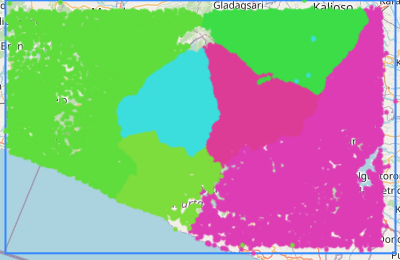
\includegraphics[]{figures/partition_level_4.png}
    \caption{Partisi hasil algoritma Inertial Flow dengan ukuran minimum partisi $U=2^{17}$ untuk graf jaringan jalan peta Openstreetmap wilayah Surakarta, Daerah Istimewa Yogyakarta, dan Klaten. Graf memiliki jumlah simpul sebanyak 481.978 dan jumlah sisi sebanyak 1.222.793.}
    \label{fig:inertial-flow}
\end{figure}

%-----------------------------------------------------------------
% Akhir BAB 3
%-----------------------------------------------------------------


%-----------------------------------------------------------------
% Awal BAB 4
%-----------------------------------------------------------------
\chapter{ANALISIS DAN PERANCANGAN SISTEM}
\label{ANALISIS DAN PERANCANGAN SISTEM}

	\section{Deskripsi Umum Sistem}
	\label{rancangan deskripsi umum sistem}
	\input{BAB_SKRIPSI/BAB4/1_DESKRIPSI_UMUM}

	\section{Analisis Kebutuhan Sistem}
	\label{rancangan analisis kebutuhan sistem}
	\input{BAB_SKRIPSI/BAB4/2_ANALISIS_KEBUTUHAN_SISTEM}

	\section{Pembuatan Sistem}
	\label{rancangan pembuatan sistem}

		\subsection{Pembuatan Sistem Pengenalan Entitas Bernama}
		\label{rancangan pembuatan sistem pengenalan entitas bernama}
		\input{BAB_SKRIPSI/BAB4/3_2_SISTEM_PENGENALAN_ENTITAS_BERNAMA}

		\subsection{Pembuatan Sistem Ekstraksi Kalimat Pernyataan}
		\label{rancangan sistem ekstraksi kalimat pernyataan}
		\input{BAB_SKRIPSI/BAB4/3_3_SISTEM_EKSTRAKSI_KALIMAT_PERNYATAAN}

	\section{Rancangan Antarmuka}
	\label{rancangan antarmuka}

		\subsection{Deskripsi}
		\label{rancangan deskripsi antarmuka}
		\input{BAB_SKRIPSI/BAB4/4_1_DESKRIPSI_RANCANGAN_ANTARMUKA}

		\subsection{\textit{Wireframe}}
	    \label{rancangan wireframe antarmuka}
	    \input{BAB_SKRIPSI/BAB4/4_2_WIREFRAME_ANTARMUKA}

%-----------------------------------------------------------------
% Akhir BAB 4
%-----------------------------------------------------------------


%-----------------------------------------------------------------
% Awal BAB 5
%-----------------------------------------------------------------
\chapter{IMPLEMENTASI SISTEM}
\label{IMPLEMENTASI SISTEM}

	\section{Spesifikasi}
	\label{implementasi spesifikasi}
	\input{BAB_SKRIPSI/BAB5/1_SPESIFIKASI}

	\section{Implementasi Sistem Pengenalan Entitas Bernama}
	\label{implementasi sistem ner}
	\input{BAB_SKRIPSI/BAB5/2_1_IMPLEMENTASI_SISTEM_NER}

	\section{Implementasi Sistem Ekstraksi Kalimat Pernyataan}
	\label{implementasi sistem ekstraksi kalimat pernyataan}
	\input{BAB_SKRIPSI/BAB5/2_2_IMPLEMENTASI_SISTEM_EKTRAKSI_KALIMAT_PERNYATAAN}

%-----------------------------------------------------------------
% Akhir BAB 5
%-----------------------------------------------------------------



%-----------------------------------------------------------------
% Awal BAB 6
%-----------------------------------------------------------------
\chapter{PENGUJIAN DAN PEMBAHASAN SISTEM}
\label{PENGUJIAN DAN PEMBAHASAN SISTEM}
\input{BAB_SKRIPSI/BAB6/1_PENDAHULUAN}

	\section{Pengujian Sistem Pengenalan Entitas Bernama}
	\label{pengujian sistem ner}
	\input{BAB_SKRIPSI/BAB6/2_PENGUJIAN_SISTEM_NER}

	\section{Pengujian Sistem Ekstraksi Kalimat Pernyataan}
	\label{pengujian sistem ekstraksi kalimat pernyataan}
	\input{BAB_SKRIPSI/BAB6/3_PENGUJIAN_SISTEM_EKSTRAKSI_KALIMAT_PERNYATAAN}

%-----------------------------------------------------------------
% Akhir BAB 6
%-----------------------------------------------------------------


%-----------------------------------------------------------------
% Awal BAB 7
%-----------------------------------------------------------------
\chapter{PENUTUP}
\label{PENUTUP}

	\section{Kesimpulan}
	\label{penutup kesimpulan}
	\input{BAB_SKRIPSI/BAB7/1_KESIMPULAN}

	\section{Saran}
	\label{penutup saran}
	\input{BAB_SKRIPSI/BAB7/2_SARAN}

%-----------------------------------------------------------------
% Akhir BAB 7
%-----------------------------------------------------------------

%-----------------------------------------------------------------
% Awal Daftar Pustaka
%-----------------------------------------------------------------
\begin{thebibliography}{99}
	\addcontentsline{toc}{chapter}{DAFTAR PUSTAKA}
    
        \bibitem[Delling et al. (2015)]{Delling2015}
        Delling, D. et al. (2015) “Customizable Route Planning in Road Networks,” \textit{Transportation Science} [Preprint]. Available at: https://doi.org/10.1287/trsc.2014.0579.

       
        \bibitem[Delling et al. (2009)]{Delling2009}
        Delling, D. et al. (2009) “Engineering Route Planning Algorithms,” in J. Lerner, D. Wagner, and K.A. Zweig (eds.) \textit{Algorithmics of Large and Complex Networks: Design, Analysis, and Simulation}. Berlin, Heidelberg: Springer, pp. 117–139. Available at: https://doi.org/10.1007/978-3-642-02094-0\_7.

          
        \bibitem[Bast et al. (2015)]{Bast2015}
        Bast, H. et al. (2015) “\textit{Route Planning in Transportation Networks.}” arXiv. Available at: https://doi.org/10.48550/arXiv.1504.05140.


        \bibitem[Baum et al. (2016)]{Baum2016}
        Baum, M. et al. (2016) “Dynamic Time-Dependent Route Planning in Road Networks with User Preferences,” in A.V. Goldberg and A.S. Kulikov (eds.) Experimental Algorithms. Cham: Springer International Publishing, pp. 33–49. Available at: https://doi.org/10.1007/978-3-319-38851-9\_3.


        \bibitem[Dijkstra et al. (1959)]{Dijkstra59}
        Dijkstra, E.W. (1959) “\textit{A note on two problems in connexion with graphs},” \textit{Numerische Mathematik}, 1(1), pp. 269–271. Available at: https://doi.org/10.1007/BF01386390.

        \bibitem[Delling dan Wagner (2009)]{DellingTD2009}
        Delling, D. and Wagner, D. (2009) “Time-Dependent Route Planning,” in R.K. Ahuja, R.H. Möhring, and C.D. Zaroliagis (eds.) \textit{Robust and Online Large-Scale Optimization: Models and Techniques for Transportation Systems}. Berlin, Heidelberg: Springer, pp. 207–230. Available at: https://doi.org/10.1007/978-3-642-05465-5\_8.

        
        
        \bibitem[Veit et al. (2013)]{Veit2013}
        Veit, B. et al. (2013) “Minimum time-dependent travel times with contraction hierarchies,” \textit{Journal of Experimental Algorithmics} (JEA) [Preprint]. Available at: https://doi.org/10.1145/2444016.2444020.


        \bibitem[Newson dan Krumm (2009)]{Newson2009}
        Newson, P. and Krumm, J. (2009) “Hidden Markov Map Matching Through Noise and Sparseness,” in. 17th \textit{ACM SIGSPATIAL International Conference on Advances in Geographic Information Systems} (ACM SIGSPATIAL GIS 2009), November 4-6, Seattle, WA, pp. 336–343. Available at: https://www.microsoft.com/en-us/research/publication/hidden-markov-map-matching-noise-sparseness/ (Accessed: September 30, 2025).


        \bibitem[Taguchi et al. (2019)]{Taguchi2019}
        Taguchi, S., Koide, S. and Yoshimura, T. (2019) “Online Map Matching With Route Prediction,” \textit{IEEE Transactions on Intelligent Transportation Systems}, 20(1), pp. 338–347. Available at: https://doi.org/10.1109/TITS.2018.2812147.

        \bibitem[Luxen dan Vetter (2011)]{Luxen2011}
        Luxen, D. and Vetter, C. (2011) ‘Real-time routing with OpenStreetMap data’, Proceedings of the 19th \textit{ACM SIGSPATIAL International Conference on Advances in Geographic Information Systems }(GIS 2011). New York: ACM, pp. 513–516.

        \bibitem[Goldberg dan Harrelson (2005)]{Goldberg2005}
        Goldberg, A. and Harrelson, C. (2005) “Computing the shortest path: A search meets graph theory,” in. ACM-SIAM Symposium on Discrete Algorithms. Vancouver: ACM, pp. 156 - 165.
        
        \bibitem[Delling et al. (2009)]{DellingHPML}
        Delling, D., Holzer, M., Müller, K., Schulz, F. and Wagner, D. (2009) ‘High-performance multi-level routing’, in The Shortest Path Problem: Ninth DIMACS Implementation Challenge. DIMACS Book, vol. 74. American Mathematical Society, pp. 73–92.

        \bibitem[Geisberger et al. (2012)]{Geisberger2012}
        Geisberger, R. et al. (2012) “Exact Routing in Large Road Networks Using Contraction Hierarchies,” Transportation Science, 46(3), pp. 388–404. Available at: https://doi.org/10.1287/trsc.1110.0401.

        \bibitem[Abaraham et al. (2011)]{Abraham2011}
        Abraham, I. et al. (2011) “A Hub-Based Labeling Algorithm for Shortest Paths in Road Networks,” in P.M. Pardalos and S. Rebennack (eds.) Experimental Algorithms. Berlin, Heidelberg: Springer, pp. 230–241. Available at: https://doi.org/10.1007/978-3-642-20662-7\_20.


        \bibitem[Gutman (2004)]{Gutman2004}
        Gutman, R.J., (2004). Reach-based routing: A new approach to shortest path algorithms optimized for road networks. In: Proceedings of the 6th Workshop on Algorithm Engineering and Experiments (ALENEX’04). SIAM, pp.100–111.

        \bibitem[Arz et al. (2013)]{Arz2013}
        Arz, J., Luxen, D. and Sanders, P. (2013) “Transit Node Routing Reconsidered,” in V. Bonifaci, C. Demetrescu, and A. Marchetti-Spaccamela (eds.) Experimental Algorithms. Berlin, Heidelberg: Springer, pp. 55–66. Available at: https://doi.org/10.1007/978-3-642-38527-8\_7.

        \bibitem[Newson dan Krumm (2009)]{Krumm2009}
        Newson, P. \& Krumm, J., (2009). "Hidden Markov map matching through noise and sparseness". Proceedings of the 17th ACM SIGSPATIAL International Conference on Advances in Geographic Information Systems (GIS ‘09), pp.336–343.

        \bibitem[Murphy (2023)]{Murphy2023}
        Murphy, K.P. (2023) Probabilistic Machine Learning: Advanced Topics. Cambridge, MA: The MIT Press.

        \bibitem[Wei et al. (2012)]{Wei2012}
        Wei, H. et al. (2012) "Fast Viterbi map matching with tunable weight functions", Proceedings of the 20th ACM SIGSPATIAL International Conference on Advances in Geographic Information Systems (ACM GIS '12), p. 613.

        \bibitem[Liang et al. (2016)]{Liang2016}
        Liang, B. et al. (2016) “Online Learning for Accurate Real-Time Map Matching,” in J. Bailey et al. (eds.) Advances in Knowledge Discovery and Data Mining. Cham: Springer International Publishing, pp. 67–78. Available at: https://doi.org/10.1007/978-3-319-31750-2\_6.
    
        \bibitem[Jagadeesh dan Srikanthan (2017)]{Jagadeesh2017}
        Jagadeesh, G.R. and Srikanthan, T. (2017) “Online Map-Matching of Noisy and Sparse Location Data With Hidden Markov and Route Choice Models,” IEEE Transactions on Intelligent Transportation Systems, 18(9), pp. 2423–2434. Available at: https://doi.org/10.1109/TITS.2017.2647967.


        \bibitem[Huang et al. (2022)]{Huang2022}
        Huang, L. et al. (2022) “An Incremental Map Matching Approach with Speed Estimation Constraints for High Sampling Rate Vehicle Trajectories,” in 2022 IEEE 17th International Conference on Control \& Automation (ICCA). 2022 IEEE 17th International Conference on Control \& Automation (ICCA), pp. 758–765. Available at: https://doi.org/10.1109/ICCA54724.2022.9831841.

    
        \bibitem[Goh et al. (2012)]{Goh2012}
        Goh, C.Y. et al. (2012) “Online map-matching based on Hidden Markov model for real-time traffic sensing applications,” in 2012 15th International IEEE Conference on Intelligent Transportation Systems. 2012 15th International IEEE Conference on Intelligent Transportation Systems, pp. 776–781. Available at: https://doi.org/10.1109/ITSC.2012.6338627.

        \bibitem[Hu et al. (2023)]{Hu2023}
        Hu, H. et al. (2023) “AMM: An Adaptive Online Map Matching Algorithm,” IEEE Transactions on Intelligent Transportation Systems, 24(5), pp. 5039–5051. Available at: https://doi.org/10.1109/TITS.2023.3237519.

        \bibitem[Cooke dan Halsey (1966)]{Cooke1966}
        Cooke, K.L. and Halsey, E. (1966) “The shortest route through a network with time-dependent internodal transit times,” Journal of Mathematical Analysis and Applications, 14(3), pp. 493–498. Available at: https://doi.org/10.1016/0022-247X(66)90009-6.


        \bibitem[Nannicini et al. (2008)]{Nannicini2008}
        Nannicini, G. et al. (2008) "Bidirectional $A^*$ Search for Time-Dependent Fast Paths," in C.C. McGeoch (ed.) Experimental Algorithms. Berlin, Heidelberg: Springer, pp. 334–346. Available at: https://doi.org/10.1007/978-3-540-68552-4\_25.
        
        \bibitem[Kohler et al. (2005)]{Kohler2005}
        Köhler, E., Möhring, R.H. and Schilling, H. (2005) “Acceleration of Shortest Path and Constrained Shortest Path Computation,” in S.E. Nikoletseas (ed.) Experimental and Efficient Algorithms. Berlin, Heidelberg: Springer, pp. 126–138. Available at: https://doi.org/10.1007/11427186\_13.

        \bibitem[Yu et al. (2018)]{Yu2018}
        Yu, B., Yin, H. and Zhu, Z. (2018) “Spatio-temporal graph convolutional networks: a deep learning framework for traffic forecasting,” in Proceedings of the 27th International Joint Conference on Artificial Intelligence. Stockholm, Sweden: AAAI Press (IJCAI’18), pp. 3634–3640.

        \bibitem[Vlahogianni (2015)]{Vlahogianni2015}
        Vlahogianni, E.I. (2015) "Computational intelligence and optimization for transportation big data: challenges and opportunities", in Engineering and Applied Sciences Optimization. Springer, pp. 107–128.        
        \bibitem[Ahmed dan Cook et al. (1979)]{AhmedCook1979}
        Ahmed, M.S. and Cook, A.R. (1979) "Analysis of freeway traffic time series data using Box and Jenkins techniques". Paper presented at the 58th Annual Meeting of the Transportation Research Board, Washington, D.C., January.


        
        \bibitem[Wang et al. (2016)]{Wang2016}
        Wang, J. et al. (2016) “Traffic Speed Prediction and Congestion Source Exploration: A Deep Learning Method,” in 2016 IEEE 16th International Conference on Data Mining (ICDM). 2016 IEEE 16th International Conference on Data Mining (ICDM), pp. 499–508. Available at: https://doi.org/10.1109/ICDM.2016.0061.


        \bibitem[Zhongjian et al. (2018)]{Zhongjian2018}
        Zhongjian Lv, et al. (2018). "LC-RNN: A deep learning model for traffic speed prediction. In 2018 International Joint Conference on Artificial Intelligence (IJCAI)". 3470–3476.
        pp. 3470 - 3476. DOI:https://doi.org/10.24963/ijcai.2018/482


        \bibitem[Yu et al. (2018)]{Yu2018}
        Yu, et al. (2018). "Spatio-temporal graph convolutional networks: A deep learning framework for traffic forecasting". In Proceedings of the 27th International Joint Conference on Artificial Intelligence. pp. 3634–3640. DOI: https://doi.org/10.24963/ijcai.2018/505.

        \bibitem[Gehring, J. et al. (2017)]{Gehring2017}
        Gehring, J. et al. (2017) ‘Convolutional sequence to sequence learning’, Proceedings of the 34th International Conference on Machine Learning (ICML 2017), 70, pp. 1243–1252

        \bibitem[Wu, J. et al. (2019)]{Wu2019}
        Wu, Z. et al. (2019) "Graph WaveNet for deep spatial-temporal graph modeling", Proceedings of the 28th International Joint Conference on Artificial Intelligence. AAAI Press, pp. 1907–1913.

        \bibitem[Pan, Z. et al. (2019)]{Pan2019}
        Pan, Z. et al. (2019) "Urban traffic prediction from spatio-temporal data using deep meta learning", *Proceedings of the 25th ACM SIGKDD International Conference on Knowledge Discovery \& Data Mining$*$, Anchorage, AK, USA, pp. 1720–1730.


        \bibitem[Guo, S. et. al. (2019)]{Guo2019}
        Guo, S. et al. (2019) "Attention Based Spatial-Temporal Graph Convolutional Networks for Traffic Flow Forecasting," Proceedings of the AAAI Conference on Artificial Intelligence, 33(01), pp. 922–929. Available at: https://doi.org/10.1609/aaai.v33i01.3301922.

        \bibitem[Bai, L. et al. (2020)]{Bai2020}
        Bai, L. et al. (2020) "Adaptive graph convolutional recurrent network for traffic forecasting", Proceedings of the 34th International Conference on Neural Information Processing Systems. Red Hook, NY: Curran Associates Inc., Article 1494, 12 pp.

        \bibitem[GraphHopper GmbH. (2025)]{Graphopper}
        GraphHopper GmbH. (2025) GraphHopper: Open source route planning library (v10.2). [Software]. Available at: https://github.com/graphhopper/graphhopper (Accessed: 10 October 2025).

        \bibitem[Luxen dan Vetter (2011)]{Luxen2011}
        Luxen, D. and Vetter, C. (2011) "Real-time routing with OpenStreetMap data", Proceedings of the 19th ACM SIGSPATIAL International Conference on Advances in Geographic Information Systems (GIS '11), Chicago, Illinois, pp. 513–516. ACM. doi: 10.1145/2093973.2094062.

        \bibitem[Valhalla contributors. (2018)]{Valhalla}
       Valhalla contributors. (2018). Valhalla: Open Source Routing Engine for OpenStreetMap (3.5.1). [software]. Mapillary AB, Mapzen. Available at: https://github.com/valhalla/valhalla [Accessed 10 October 2025].

        \bibitem[Schild dan Sommer et al. (2015)]{Schild2015}
       Schild, A. and Sommer, C. (2015) “On Balanced Separators in Road Networks,” in E. Bampis (ed.) Experimental Algorithms. Cham: Springer International Publishing, pp. 286–297. Available at: https://doi.org/10.1007/978-3-319-20086-6\_22.

    \bibitem[Haeupler et al. (2009)]{Haeupler2009}
    Haeupler, B., Sen, S. and Tarjan, R.E. (2009) “Rank-Pairing Heaps,” in A. Fiat and P. Sanders (eds.) Algorithms - ESA 2009. Berlin, Heidelberg: Springer, pp. 659–670. Available at: https://doi.org/10.1007/978-3-642-04128-0\_59.

    \bibitem[Wu et al. (2020)]{Wu2020}
    Wu, Z. et al. (2020) "Connecting the Dots: Multivariate Time Series Forecasting with Graph Neural Networks," in Proceedings of the 26th ACM SIGKDD International Conference on Knowledge Discovery \& Data Mining. New York, NY, USA: Association for Computing Machinery (KDD '20), pp. 753–763. Available at: https://doi.org/10.1145/3394486.3403118.

    \bibitem[Abraham et al. (2010)]{Abraham2010}
    Abraham, I. et al. (2010) “Alternative Routes in Road Networks,” in P. Festa (ed.) Experimental Algorithms. Berlin, Heidelberg: Springer, pp. 23–34. Available at: https://doi.org/10.1007/978-3-642-13193-6\_3.

    \bibitem[Dinitz et al. (2006)]{Dinitz2006}
    Dinitz, Y. (2006) “Dinitz' Algorithm: The Original Version and Even’s Version,” in O. Goldreich, A.L. Rosenberg, and A.L. Selman (eds.) Theoretical Computer Science: Essays in Memory of Shimon Even. Berlin, Heidelberg: Springer, pp. 218–240. Available at: https://doi.org/10.1007/11685654\_10.


    \bibitem[Cormen et al. (2022)]{Cormen2022}
    Cormen, T.H. et al. (2022) Introduction to Algorithms. 4th ed. Cambridge, MA, USA: MIT Press.

\end{thebibliography}   

%-----------------------------------------------------------------
% Akhir Daftar Pustaka
%-----------------------------------------------------------------


%-----------------------------------------------------------------
% Awal lampiran
%-----------------------------------------------------------------
\appendix

\chapter{BERKAS JSON UNTUK MODEL SISTEM PENGENALAN ENTITAS BERNAMA}
\label{BERKAS JSON UNTUK MODEL SISTEM PENGENALAN ENTITAS BERNAMA}
\input{BAB_SKRIPSI/BAB9_LAMPIRAN/1_BERKAS_MODEL_NER}

%-----------------------------------------------------------------
% Akhir lampiran
%-----------------------------------------------------------------

\end{document}